\chapter{Analisis}
\label{chap:analisis}

% label: {what for}:{page}:{section}:{subsection}:{name}

\section{Analisis Sistem Kini}
\label{sec:3:sistemkini}

Seperti yang sudah dibahas pada subbab \ref{sec:2:sharifjudge}, SharIF Judge merupakan sebuah website judge yang dimodifikasi sesuai dengan kebutuhan Teknik Informatika UNPAR. Analisis diawali dengan MVC aplikasi SharIF Judge. Berikut merupakan hasil eksplorasi SharIF Judge yang telah dilakukan:

\subsection{Model, View, Controller}
\label{sub:3:1:modelviewcontroller}

SharIF Judge menggunakan \textit{framework} CodeIgniter 3 yang berbasis arsitektur Model-View-Controller seperti yang dijelaskan pada subbab \ref{sub:2:2:modelviewcontroller}. Gambar \ref{fig:3:1:mvc} merupakan kelas diagram struktur MVC pada SharIF Judge. Berikut merupakan hasil eksplorasi dari struktur MVC pada SharIF Judge:

\begin{figure}
	\centering
	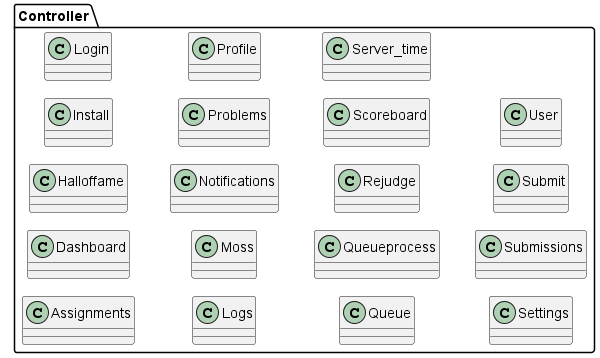
\includegraphics[width=0.55\textwidth]{analisis/class/class_controller.png}
	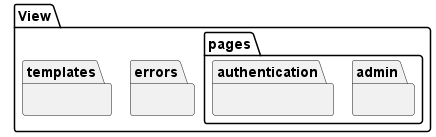
\includegraphics[width=0.4\textwidth]{analisis/class/class_view.png}
	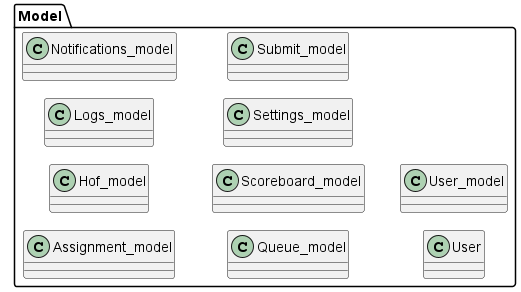
\includegraphics[width=0.55\textwidth]{analisis/class/class_model.png}
	\caption{Struktur MVC pada SharIF Judge}
	\label{fig:3:1:mvc}
\end{figure}

\subsubsection{Model}
\label{sub:3:1:1:model}

Analisis MVC akan dimulai dengan \textit{model} yang berada pada direktori \verb|application/models|. Direktori \textit{Model} berisi kelas-kelas yang digunakan untuk mengelola dan mengembalikan data dari \textit{database}.
Gambar \ref{fig:3:1:1:model} merupakan struktur kelas \textit{model} dalam SharIF Judge.
\begin{figure}
	\centering
	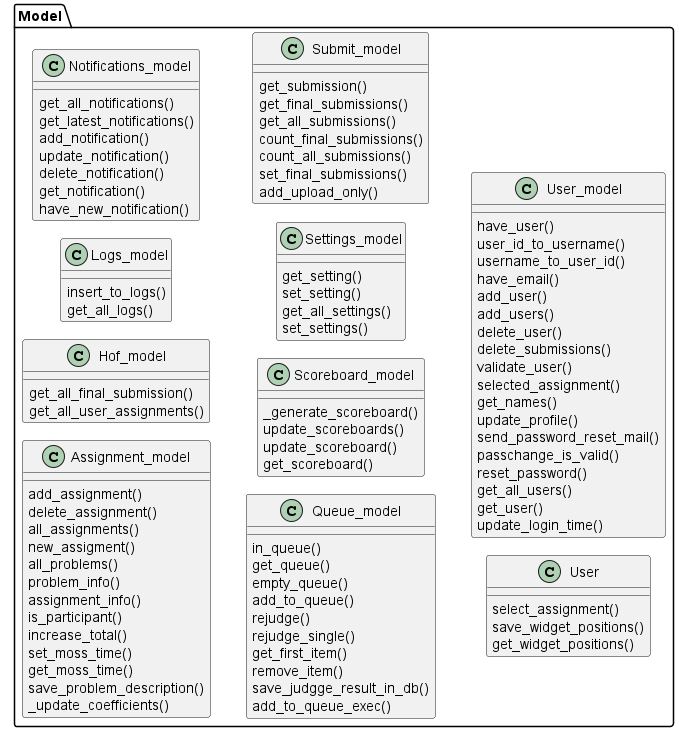
\includegraphics[width=0.65\textwidth]{analisis/mvc/model.png}
	\caption{Struktur Kelas Model pada SharIF Judge}
	\label{fig:3:1:1:model}
\end{figure}
Berikut merupakan penjelasan dari kelas \textit{model} dan fungsi-fungsinya yang terdapat pada SharIF Judge:

\begin{itemize}
	\item \verb|Assignment_model.php| \\
	      Model \verb|Assignment_model.php| digunakan untuk mengelola tabel \verb|assignments| dan mengembalikan informasi dari database yang digunakan dalam halaman \textit{assignment} dan \textit{problem}. Fungsi yang dimiliki adalah sebagai berikut:

	      \begin{itemize}
		      \item \verb|add_assignment($id, $edit)| \\
		            Menambahkan atau memperbaharui sebuah \textit{assignment}.
		      \item \verb|delete_assignment($assignment_id)| \\
		            Menghapus sebuah \textit{assignment}.
		      \item \verb|all_assignments()| \\
		            Mengembalikan daftar semua \textit{assignment} dan informasinya.
		      \item \verb|new_assignment_id()| \\
		            Mendapatkan nomor terkecil dan dapat digunakan sebagai \textit{id assignment} terbaru.
		      \item \verb|all_problems($assignment_id)| \\
		            Mengembalikan daftar semua \textit{problems} dari sebuah \textit{assignment}.
		      \item \verb|problem_info($assignment_id, $problem_id)| \\
		            Mengembalikan semua informasi sebuah \textit{problem}
		      \item \verb|assignment_info($assignment_id)| \\
		            Mengembalikan semua informasi sebuah \textit{assignment}
		      \item \verb|is_participant($participants, $username)| \\
		            Mengembalikan \textit{boolean} apakah \verb|$username| terdapat dalam \verb|$participants|.
		      \item \verb|increase_total_submits($assignment_id)| \\
		            Menambahkan jumlah \textit{total submits} sebanyak satu pada sebuah assignment.
		      \item \verb|set_moss_time($assignment_id)| \\
		            Memperbaharui ``\textit{Moss Update Time}'' pada sebuah \textit{assignment}.
		      \item \verb|get_moss_time($assignment_id)| \\
		            Mengembalikan ``\textit{Moss Update Time}'' pada sebuah assignment.
		      \item \verb|save_problem_description($assignment_id, $problem_id, $text, $type)| \\
		            Menambahkan atau memperbaharui deskripsi pada sebuah \textit{problem}.
		      \item \verb|_update_coefficients($a_id, $extra_time, $finish_time, $new_late_rule)| \\
		            Memperbaharui koefisien dari sebuah \textit{assignment}.
	      \end{itemize}

	\item \verb|Hof_model.php| \\
	      Model ini digunakan untuk mengembalikan informasi yang digunakan dalam \textit{hall of fame} dari tabel \verb|submissions|. Fungsi yang dimiliki adalah sebagai berikut:

	      \begin{itemize}
		      \item \verb|get_all_final_submission()| \\
		            Mengembalikan seluruh total nilai \textit{final submission} untuk semua pengguna.
		      \item \verb|get_all_user_assignments($username)| \\
		            Mengembalikan nilai \textit{final submission} pada semua problem untuk pengguna tertentu.
	      \end{itemize}

	\item \verb|Logs_model.php| \\
	      Model ini berfungsi untuk mengelola tabel \verb|logins| dan mengembalikan catatan \textit{login}. Fungsi yang dimiliki adalah sebagai berikut:

	      \begin{itemize}
		      \item \verb|insert_to_logs($username, $ip_address)| \\
		            Mencatat \textit{login} pengguna dan menghapus catatan jika melebihi 24 jam.
		      \item \verb|get_all_logs()| \\
		            Mengembalikan semua catatan \textit{login}.
	      \end{itemize}

	\item \verb|Notifications_model.php| \\
	      Model ini digunakan untuk mengelola tabel \verb|notifications|. Fungsi yang dimiliki oleh model \verb|Notifications_model.php| adalah sebagai berikut:

	      \begin{itemize}
		      \item \verb|get_all_notifications()| \\
		            Mengembalikan semua \textit{notifications}.
		      \item \verb|get_latest_notifications()| \\
		            Mengembalikan 10 \textit{notifications} terbaru.
		      \item \verb|add_notification($title, $text)| \\
		            Menambahkan \textit{notification} baru.
		      \item \verb|update_notification($id, $title, $text)| \\
		            Memperbaharui sebuah \textit{notification}.
		      \item \verb|delete_notification($id)| \\
		            Menghapus sebuah \textit{notification}.
		      \item \verb|get_notification($notif_id)| \\
		            Mengembalikan sebuah \textit{notification}.
		      \item \verb|have_new_notification($time)| \\
		            Mengembalikan nilai \textit{boolean} yang menunjukkan apakah terdapatnya \textit{notification} baru.
	      \end{itemize}

	\item \verb|Queue_model.php| \\
	      Model ini digunakan untuk mengelola tabel \verb|queue| dan menampilkan data \verb|queue|. Fungsi yang dimiliki adalah sebagai berikut:

	      \begin{itemize}
		      \item \verb|in_queue($username, $assignment, $problem)| \\
		            Fungsi ini digunakan untuk mengembalikan sebuah \textit{boolean} yang menyatakan bahwa \textit{username} masih memiliki \textit{queue} dalam sebuah \textit{problem}.
		      \item \verb|get_queue()| \\
		            Mengambil semua \textit{submission queue}.
		      \item \verb|empty_queue()| \\
		            Menghapus semua \textit{queue}.
		      \item \verb|add_to_queue($submit_info)| \\
		            Menambahkan sebuah \textit{submission} ke dalam \textit{queue}.
		      \item \verb|rejudge($assignment_id, $problem_id)| \\
		            Fungsi ini digunakan untuk menambahkan seluruh \textit{submissions} dalam sebuah \textit{problem} ke dalam \textit{queue} untuk dinilai ulang.
		      \item \verb|rejudge_single($submission)| \\
		            menambahkan sebuah \textit{submission} ke dalam \textit{queue} untuk dinilai ulang.
		      \item \verb|get_first_item()| \\
		            Mengembalikan \textit{item} pertama dalam tabel \verb|queue|.
		      \item \verb|remove_item($username, $assignment, $problem, $submit_id)| \\
		            Menghapus sebuah \textit{item} tertentu dalam tabel \verb|queue|.
		      \item \verb|save_judge_result_in_db ($submission, $type)| \\
		            Menyimpan hasil penilaian \textit{judge} ke dalam \textit{database}.
		      \item \verb|add_to_queue_exec($submit_info)| \\
		            Fungsi ini digunakan untuk menambahkan sebuah \textit{dummy submission} dari IDE yang digunakan hanya untuk dijalankan ke dalam \textit{queue}.
	      \end{itemize}

	\item \verb|Scoreboard_model.php| \\
	      Model ini digunakan untuk mengelola tabel \verb|scoreboard|. Fungsi yang dimiliki oleh \textit{model} \verb|Scoreboard_model.php| adalah sebagai berikut:

	      \begin{itemize}
		      \item \verb|_generate_scoreboard($assignment_id)| \\
		            Menghasilkan \textit{scoreboard} untuk sebuah \textit{assignment} dari nilai akhir semua \textit{submission}.
		      \item \verb|update_scoreboards()| \\
		            Memperbaharui \textit{scoreboard} untuk semua \textit{assignment}.
		      \item \verb|update_scoreboard($assignment_id)| \\
		            Memperbaharui \textit{scoreboard} untuk sebuah \textit{assignment}.
		      \item \verb|get_scoreboard($assignment_id)| \\
		            Mengembalikan \textit{scoreboard} pada sebuah \textit{assignment}.
	      \end{itemize}

	\item \verb|Settings_model.php| \\
	      Model ini digunakan untuk mengelola tabel \verb|settings|. Fungsi yang dimiliki oleh \textit{model} \\\verb|Settings_model.php| adalah sebagai berikut:

	      \begin{itemize}
		      \item \verb|get_setting($key)| \\
		            Mengembalikan nilai dari sebuah \verb|$key| pada tabel \verb|settings|.
		      \item \verb|set_setting($key, $value)| \\
		            Memperbaharui nilai dari pada \textit{setting} \verb|$key|.
		      \item \verb|get_all_settings()| \\
		            Mengembalikan seluruh \textit{settings}.
		      \item \verb|set_settings($settings)| \\
		            Memperbaharui seluruh nilai perubahan \textit{settings}.
	      \end{itemize}

	\item \verb|Submit_model.php| \\
	      Model ini digunakan untuk mengelola tabel \verb|submission|. Fungsi yang dimiliki oleh \textit{model} \verb|Submit_model.php| adalah sebagai berikut:

	      \begin{itemize}
		      \item \verb|get_submission($username, $assignment, $problem, $submit_id)| \\
		            Mengembalikan sebuah baris data \textit{submission} tertentu.
		      \item \verb|get_final_submissions($a_id, $u_vl, $uname, $p_num, $fil_u, $fil_prob)| \\
		            Mengembalikan seluruh \textit{final submission} pada sebuah \textit{assignment}. pengguna dengan role \textit{student} hanya dapat melihat \textit{final submission} dirinya sendiri.
		      \item \verb|get_all_submissions($a_id, $u_vl, $uname, $p_num, $fil_u, $fil_prob)| \\
		            Mengembalikan seluruh \textit{submission} pada sebuah \textit{assignment}. pengguna dengan role \textit{student} hanya dapat melihat \textit{submission} dirinya sendiri.
		      \item \verb|count_final_submissions($a_id, $u_vl, $uname, $fil_u, $fil_prob)| \\
		            Mengembalikan jumlah \textit{final submission} pada sebuah \textit{assignment}.
		      \item \verb|count_all_submissions($a_id, $u_vl, $uname, $fil_u, $fil_prob)| \\
		            Mengembalikan jumlah \textit{submission} pada sebuah \textit{assignment}.
		      \item \verb|set_final_submission($username, $assignment, $problem, $submit_id)| \\
		            Memperbaharui sebuah \textit{submission} menjadi \textit{final submission}.
		      \item \verb|add_upload_only($submit_info)| \\
		            Menyimpan hasil \textit{upload only problem} ke dalam tabel \textit{database}.
	      \end{itemize}

	\item \verb|User.php| \\
	      Model ini digunakan untuk menyimpan \textit{settings} sebuah pengguna. Fungsi yang dimiliki oleh \textit{model} \verb|User.php| adalah sebagai berikut:

	      \begin{itemize}
		      \item \verb|select_assignment($assignment_id)| \\
		            Menyimpan \textit{assignment} yang dipilih oleh pengguna.
		      \item \verb|save_widget_positions($positions)| \\
		            Menyimpan posisi \textit{widget} sebuah pengguna.
		      \item \verb|get_widget_positions()| \\
		            Mendapatkan posisi \textit{widget} sebuah pengguna.
	      \end{itemize}

	\item \verb|User_model.php| \\
	      Model \verb|User_model.php| digunakan untuk mengelola tabel \verb|users|. Fungsi yang dimiliki oleh \textit{model} \verb|User_model.php| adalah sebagai berikut:

	      \begin{itemize}
		      \item \verb|have_user($username)| \\
		            Mengembalikan sebuah \textit{boolean} yang menyatakan \verb|$username| sudah ada pada \textit{database}.
		      \item \verb|user_id_to_username($user_id)| \\
		            Mengembalikan \textit{username} dari \verb|$user_id|.
		      \item \verb|username_to_user_id($username)| \\
		            Mengembalikan \textit{user id} dari \verb|$username|.
		      \item \verb|have_email($email, $username)| \\
		            Mengembalikan \textit{boolean} yang menyatakan jika pengguna memiliki \textit{email} pada \textit{database}.
		      \item \verb|add_user($username, $email, $display_name, $password, $role)| \\
		            Menambahkan satu pengguna baru ke dalam \textit{database}.
		      \item \verb|add_users($text, $send_mail, $delay)| \\
		            Menambahkan banyak pengguna baru ke dalam \textit{database}.
		      \item \verb|delete_user($user_id)| \\
		            Menghapus sebuah pengguna dalam \textit{database}.
		      \item \verb|delete_submissions($user_id)| \\
		            Mendelete semua \textit{submissions} yang di \textit{submit} oleh sebuah pengguna.
		      \item \verb|validate_user($username, $password)| \\
		            Mengembalikan sebuah \textit{boolean} yang menyatakan bahwa \verb|$password| dan \verb|$username|
		      \item \verb|selected_assignment($username)| \\
		            Mengembalikan \textit{assignment} yang dipilih oleh \verb|$username|.
		      \item \verb|get_names()| \\
		            Mengembalikan semua \textit{display name} pada tabel \textit{users}.
		      \item \verb|update_profile($user_id)| \\
		            Memperbaharui nama, email, password, atau role sebuah pengguna.
		      \item \verb|send_password_reset_mail($email)| \\
		            Mengirimkan \textit{link reset password} ke email pengguna yang dapat dipakai selama 1 jam.
		      \item \verb|passchange_is_valid($passchange_key)| \\
		            Fungsi ini digunakan untuk mengembalikan sebuah \textit{boolean} yang menyatakan bahwa \textit{link reset password} yang diberikan dapat digunakan atau tidak.
		      \item \verb|reset_password($passchange_key, $newpassword)| \\
		            Memperbaharui \textit{password} dengan divalidasinya \textit{password change key}.
		      \item \verb|get_all_users()| \\
		            Mengembalikan seluruh pengguna pada tabel \verb|users|.
		      \item \verb|get_user($user_id)| \\
		            Mengembalikan sebuah pengguna yang memiliki id \verb|$user_id|.
		      \item \verb|update_login_time($username)| \\
		            Memperbaharui catatan \textit{login} untuk sebuah pengguna.
	      \end{itemize}
\end{itemize}

\vspace{-0.5cm}

\subsubsection{View}
\label{sub:3:1:1:view}

\textit{View} merupakan tampilan yang menjadi perantara antara pengguna dan \textit{sistem}. Pada SharIF Judge, \textit{View} disimpan pada direktori \verb|application/views| dan dibagi menjadi 3 direktori terpisah yaitu errors, pages, dan template.
Gambar \ref{fig:3:1:1:view} merupakan struktur direktori \textit{view} beserta \textit{view} yang terdapat pada direktorinya dalam SharIF Judge.
\begin{figure}[H]
	\centering
	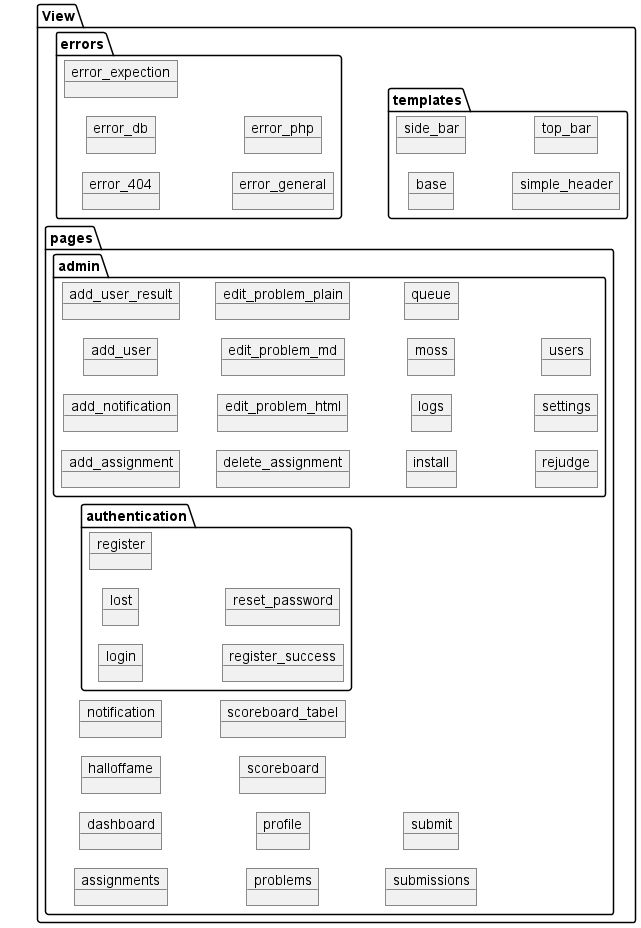
\includegraphics[width=0.6\textwidth]{analisis/mvc/view.png}
	\caption{Struktur Direktori View pada SharIF Judge}
	\label{fig:3:1:1:view}
\end{figure}
Berikut merupakan penjelasan mengenai direktori penyimpanan untuk \textit{view} pada SharIF Judge.

\begin{itemize}
	\item \verb|errors| \\
	      Pada direktori \textit{errors}, berisi tampilan halaman \textit{error} jika terjadi error pada penggunaan SharIF Judge. Berikut merupakan \textit{views} yang terdapat pada direktori \verb|errors|:

	      \begin{itemize}
		      \item \verb|error_404|
		      \item \verb|error_db|
		      \item \verb|error_exception|
		      \item \verb|error_general|
		      \item \verb|error_php|
	      \end{itemize}

	\item \verb|pages| \\
	      Pada direktori \textit{pages}, berisi tampilan halaman-halaman utama. \textit{pages} juga memiliki dua direktori selain halaman-halama. Berikut merupakan \textit{views} dan direktori pada \verb|pages|:

	      \begin{itemize}
		      \item \verb|pages/admin| \\
		            Direktori \textit{admin} berisi tampilan halaman khusus untuk \textit{role admin}. Berikut merupakan \textit{views} yang terdapat pada direktori \verb|admin|:

		            \begin{itemize}
			            \item \verb|add_assignment.twig|
			            \item \verb|add_notification.twig|
			            \item \verb|add_user.twig|
			            \item \verb|add_user_result.twig|
			            \item \verb|delete_assignment.twig|
			            \item \verb|edit_problem_html.twig|
			            \item \verb|edit_problem_md.twig|
			            \item \verb|edit_problem_plain.twig|
			            \item \verb|install.twig|
			            \item \verb|logs.twig|
			            \item \verb|moss.twig|
			            \item \verb|queue.twig|
			            \item \verb|rejudge.twig|
			            \item \verb|settings.twig|
			            \item \verb|users.twig|
		            \end{itemize}

		      \item \verb|pages/authentication| \\
		            Direktori \textit{authentication} berisi tampilan halaman khusus untuk \textit{authentication} seperti halaman direktori \textit{Login}. Berikut merupakan \textit{views} yang terdapat pada direktori \verb|admin|:

		            \begin{itemize}
			            \item \verb|login.twig|
			            \item \verb|lost.twig|
			            \item \verb|register.twig|
			            \item \verb|register_success.twig|
			            \item \verb|reset_password.twig|
		            \end{itemize}

		      \item \verb|assignments.twig|
		      \item \verb|dashboard.twig|
		      \item \verb|halloffame.twig|
		      \item \verb|notification.twig|
		      \item \verb|problems.twig|
		      \item \verb|profile.twig|
		      \item \verb|scoreboard.twig|
		      \item \verb|scoreboard_tabel.twig|
		      \item \verb|submissions.twig|
		      \item \verb|submit.twig|
	      \end{itemize}

	\item \verb|templates| \\
	      Pada direktori \textit{templates}, berisi tampilan yang digunakan berulang oleh halaman utama seperti \textit{header}, \textit{sidebar}, dan \textit{base}. Berikut merupakan \textit{views} yang terdapat pada \verb|templates|:

	      \begin{itemize}
		      \item \verb|base.twig|
		      \item \verb|side_bar.twig|
		      \item \verb|simple_header.twig|
		      \item \verb|top_bar.twig|
	      \end{itemize}

\end{itemize}

\subsubsection{Controller}
\label{sub:3:1:1:controller}

Pada bagian analisis MVC terakhir, terdapat \textit{controller} yang berada pada direktori \verb|application|\\\verb|/controller|. Seperti yang dijelaskan pada subbab \ref{sub:2:2:3:Controller}, \textit{Controller} digunakan sebagai perantara antara \textit{model}, \textit{view}, dan \textit{resources} lainnya yang dibutuhkan saat membuat sebuah web page. Direktori controller berisi kelas-kelas yang akan mengolah data yang didapat pada \textit{model} dan menyatukan data tersebut ke dalam \textit{views} yang akan ditampilkan kepada pengguna. Pada setiap kelas \textit{controller}, terdapat fungsi \verb|index()| yang menjadi fungsi utama saat kelas di akses oleh pengguna.
Gambar \ref{fig:3:1:1:controller} merupakan struktur kelas \textit{controller} yang terdapat pada SharIF Judge.
\begin{figure}[H]
	\centering
	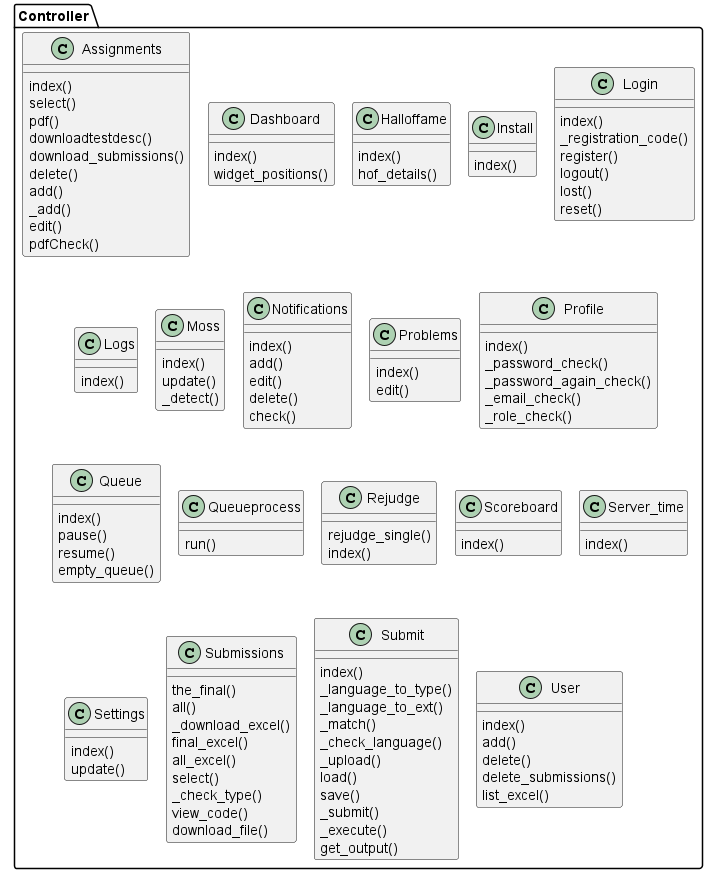
\includegraphics[width=\textwidth]{analisis/mvc/controller.png}
	\caption{Struktur Kelas Controller pada SharIF Judge}
	\label{fig:3:1:1:controller}
\end{figure}

\newpage

Berikut merupakan file \textit{controller} dan penjelasan fungsinya pada SharIF Judge:

\vspace{0.5cm}

\begin{itemize}
	\item \verb|Assignments.php| \\
	      Berikut fungsi dengan penjelasannya pada \textit{controller} \verb|Assignments.php|:


	      \begin{itemize}
		      \item \verb|select()| \\
		            Memilih \textit{assignment} yang ditampilkan pada \textit{top bar} menggunakan \textit{ajax request}.
		      \item \verb|pdf($assignment_id, $problem_id, $no_download)| \\
		            Mengunduh \textit{assignment} atau \textit{problem} dalam bentuk PDF ke browser.
		      \item \verb|downloadtestsdesc($assignment_id)| \\
		            Mengunduh dan mencompress data uji dan deskripsi sebuah \textit{assignment}.
		      \item \verb|download_submissions($type, $assignment_id)| \\
		            Mengunduh semua \textit{final submission} pada semua \textit{assignment}.
		      \item \verb|delete($assignment_id)| \\
		            Menghapus sebuah \textit{assignment}.
		      \item \verb|add()| \\
		            Mendapatkan \textit{input} dari pengguna untuk menambah atau memperbaharui \textit{assignment}.
		      \item \verb|_add()| \\
		            Menambahkan atau memperbaharui sebuah \textit{assignment}.
		      \item \verb|edit($assignment_id)| \\
		            Menandai \textit{assignment} yang akan di \textit{edit} dan memanggil fungsi \verb|add|.
		      \item \verb|pdfCheck($assignment_id, $problem_id)| \\
		            Melakukan validasi ketersediaan pdf pada sebuah \textit{assignment} atau pada sebuah \textit{problem}.
		      \item \verb|index()| \\
		            Mengambil data dari \verb|Assignment_model| dan menyimpan data dan mengembalikan \textit{views} \verb|assignments.twig|. Gambar \ref{fig:3:1:1:assignments} menunjukkan hasil halaman Assignment.

		            \vspace{0.5cm}

		            \begin{figure}[H]
			            \centering
			            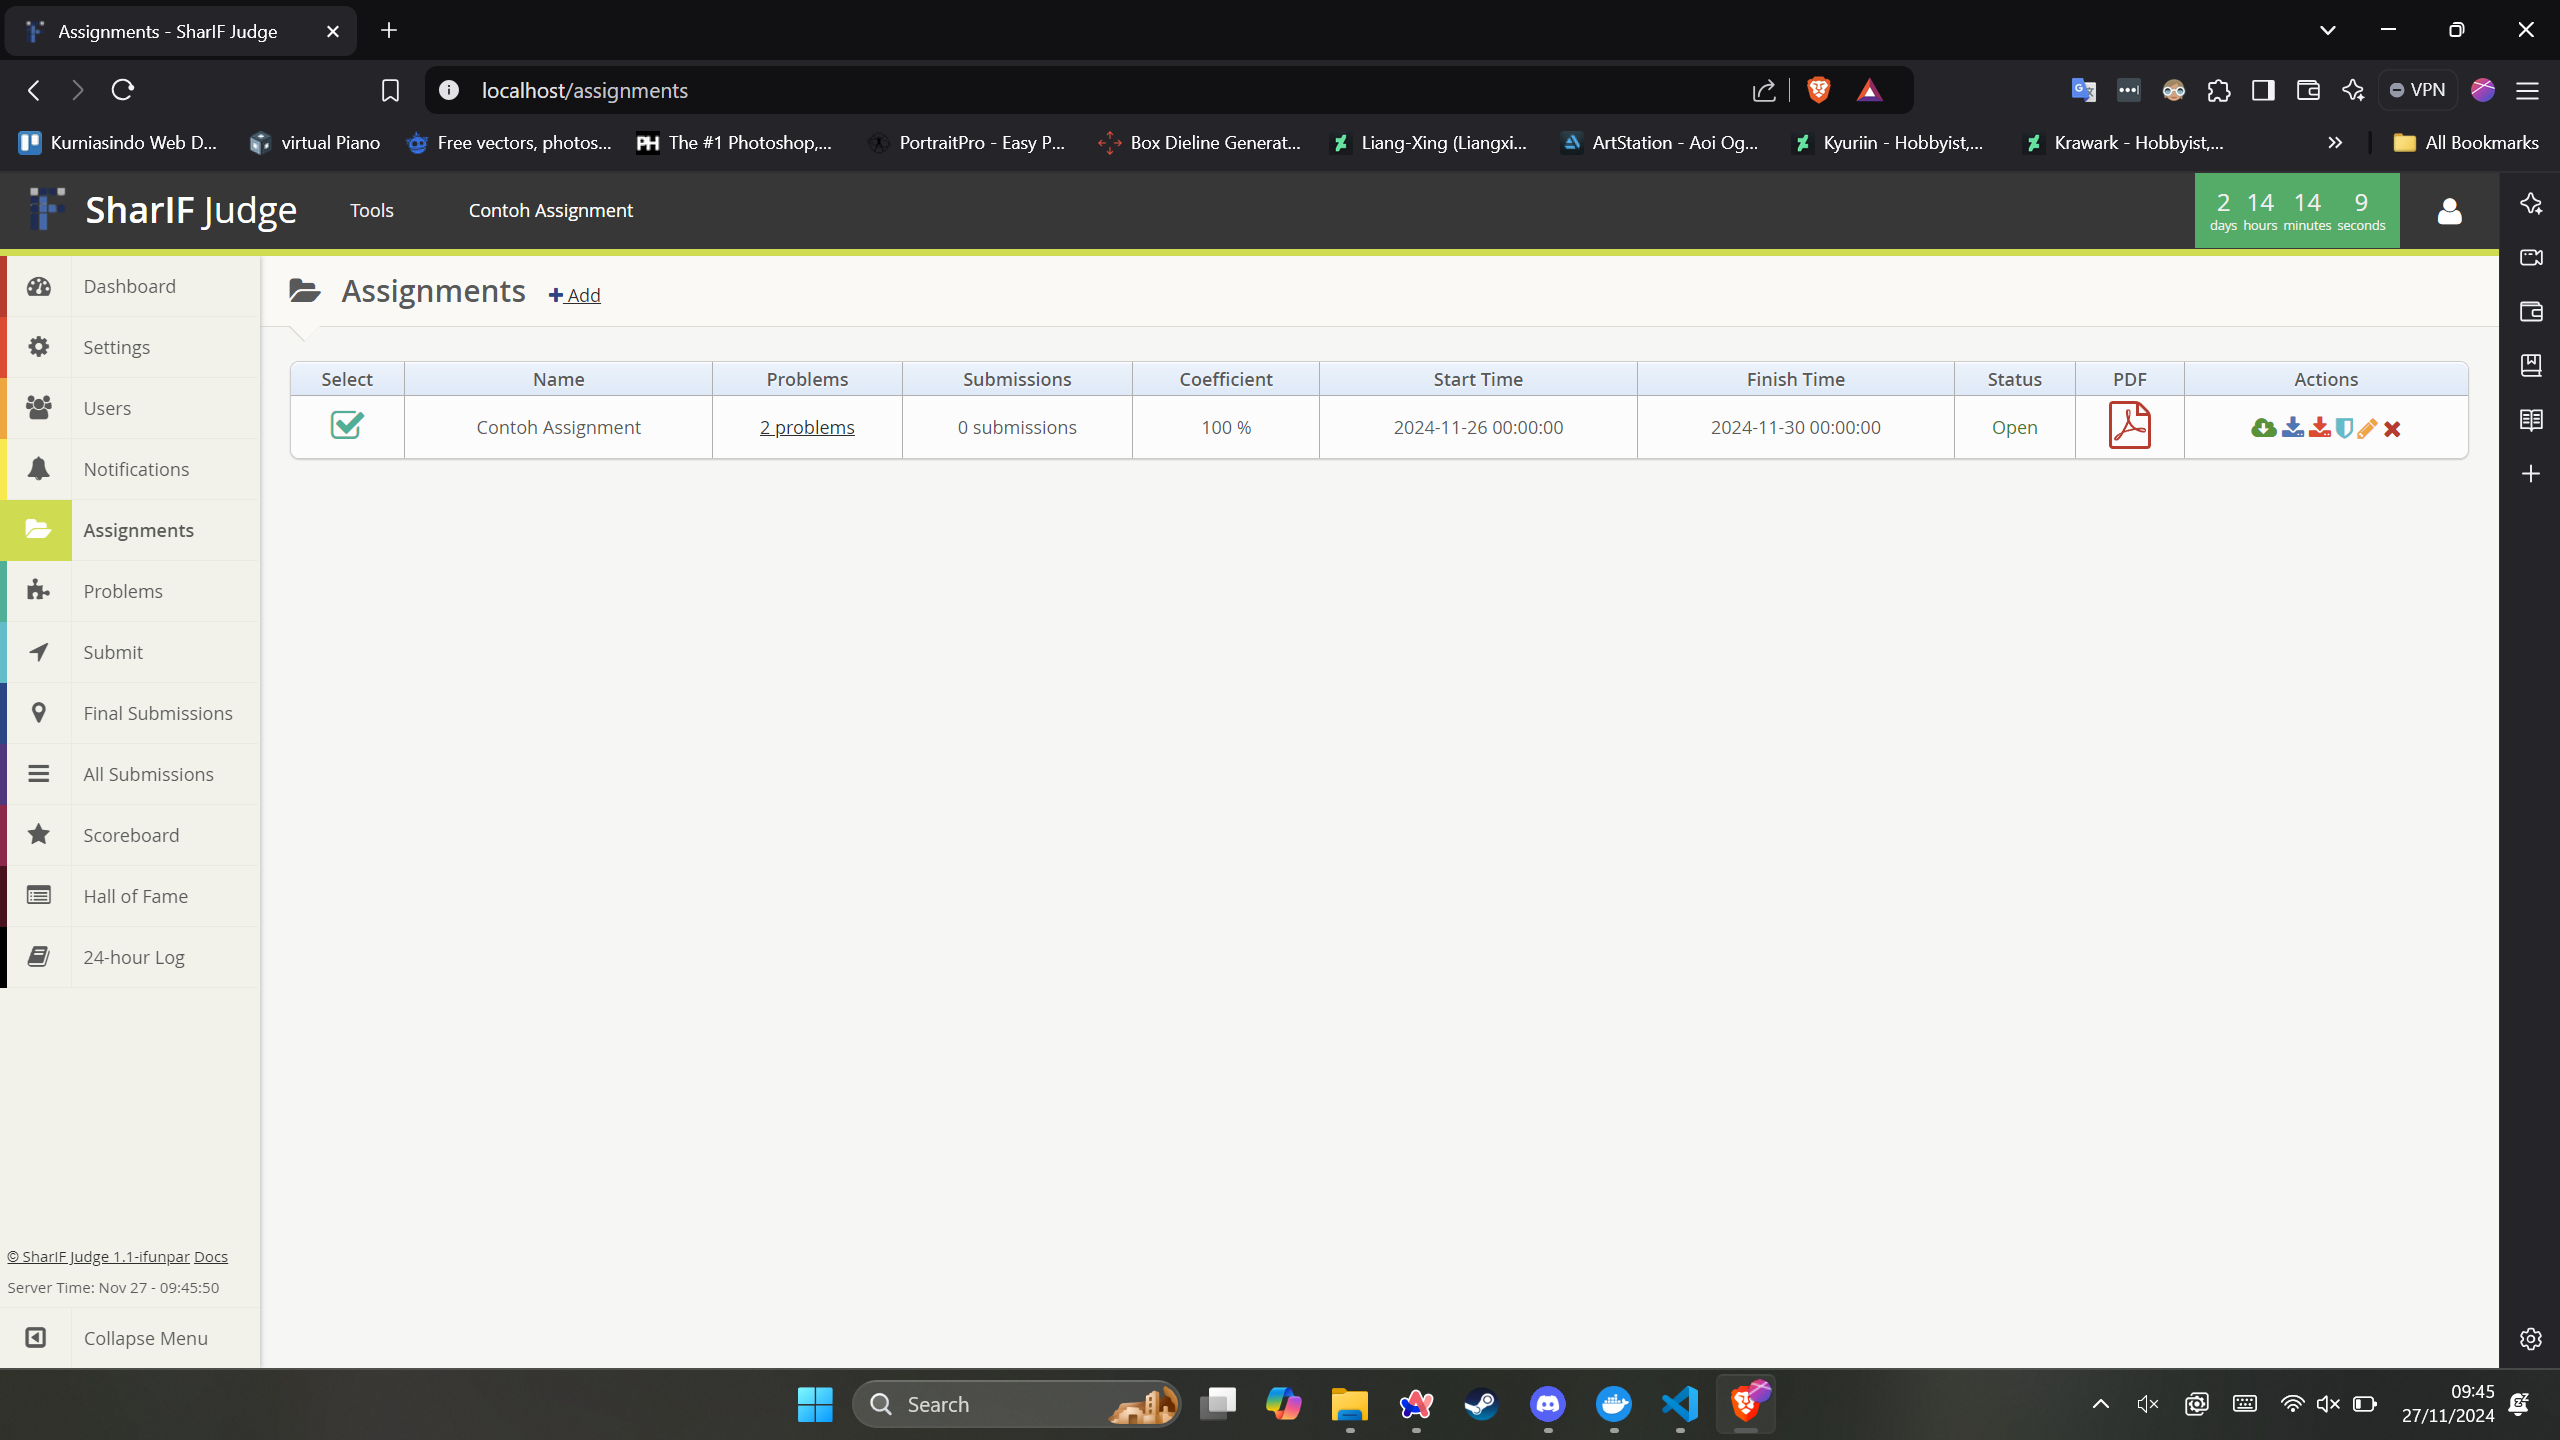
\includegraphics[width=0.9\textwidth]{views/assignments.png}
			            \caption{Halaman Assignments}
			            \label{fig:3:1:1:assignments}
		            \end{figure}
	      \end{itemize}

	\item \verb|Dashboard.php| \\
	      Berikut fungsi dengan penjelasannya pada \textit{controller} \verb|Dashboard.php|:

	      \begin{itemize}
		      \item \verb|widget_positions()| \\
		            menggunakan \textit{ajax request} untuk menyimpan posisi \textit{widget}.

		      \item \verb|index()| \\
		            Mendapatkan data dari beberapa model yaitu \verb|Assignment_model|, \verb|Settings_model|, \verb|User|, dan \verb|Notifications_model|. Data akan dimasukkan ke dalam \verb|dashboard.twig| yang akan dikembalikan ke pengguna. Gambar \ref{fig:3:1:1:dashboard} menunjukkan hasil halaman Dashboard yang dapat diakses oleh semua \textit{role}.

		            \begin{figure}[H]
			            \centering
			            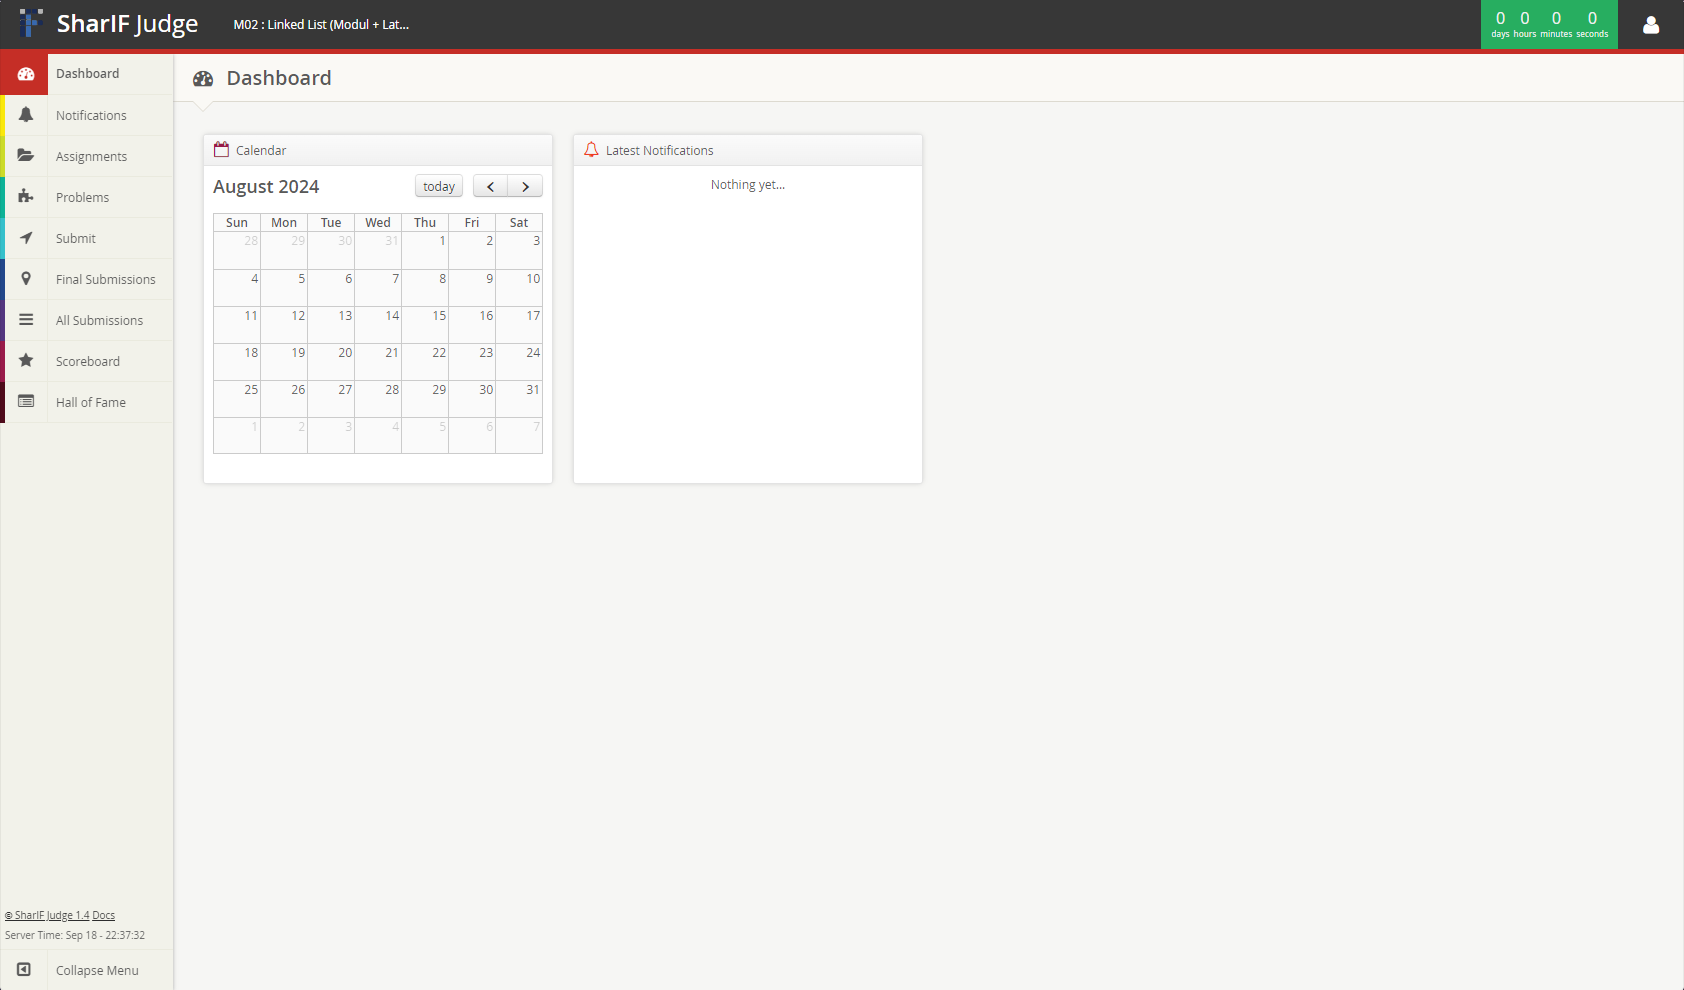
\includegraphics[width=0.65\textwidth]{views/dashboard.png}
			            \caption{Halaman Dashboard}
			            \label{fig:3:1:1:dashboard}
		            \end{figure}

	      \end{itemize}

	\item \verb|Halloffame.php| \\
	      Berikut fungsi dengan penjelasannya pada \textit{controller} \verb|Halloffame.php|:

	      \begin{itemize}
		      \item \verb|hof_details()| \\
		            Menampilkan nilai akhir semua \textit{problem} dan \textit{assignments} pada sebuah pengguna.

		      \item \verb|index()| \\
		            Mendapatkan data dari \verb|Hof_model| dan mengembalikan \textit{view} \verb|halloffame.twig|. Gambar \ref{fig:3:1:1:hof} menunjukkan hasil halaman Hall of Fame yang dapat diakses oleh semua \textit{role}.

		            \begin{figure}[H]
			            \centering
			            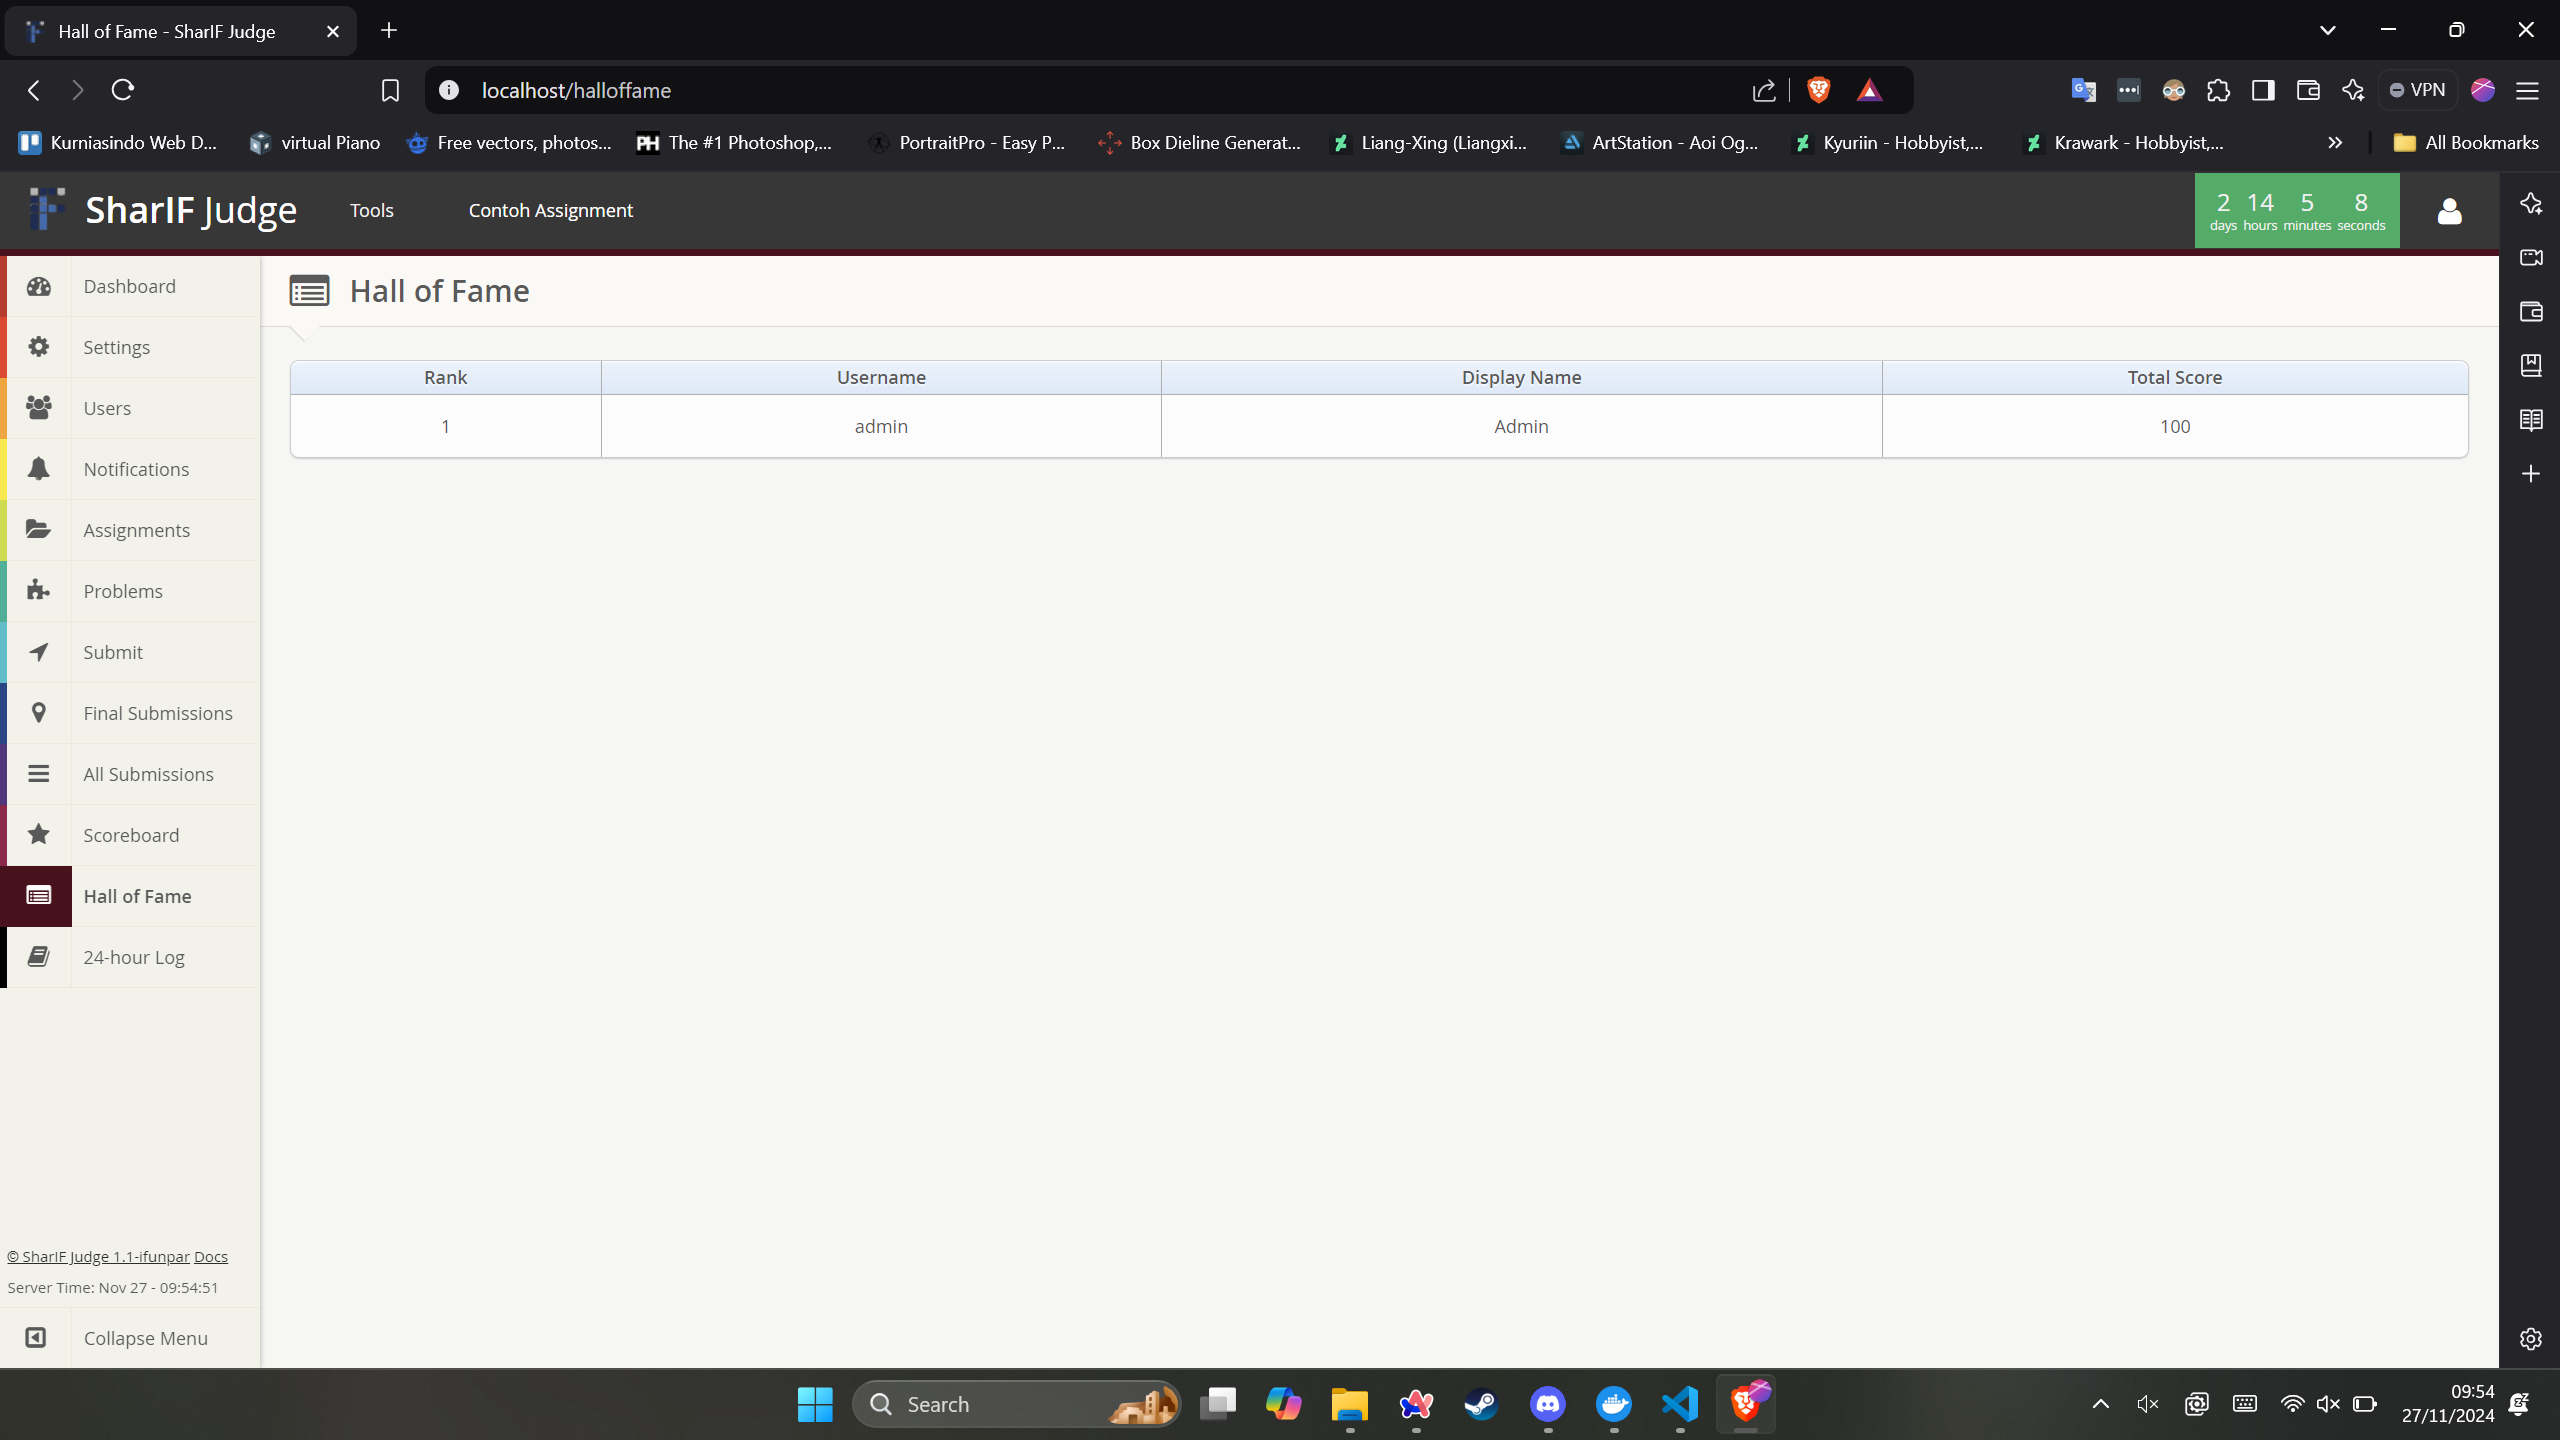
\includegraphics[width=0.65\textwidth]{views/hof.png}
			            \caption{Halaman Hall of Fame}
			            \label{fig:3:1:1:hof}
		            \end{figure}


	      \end{itemize}

	\item \verb|Install.php| \\
	      Pada \textit{controller} \verb|Install.php| hanya ada satu fungsi yang menangani pembuatan seluruh tabel pada \textit{database} yang dibutuhkan oleh SharIF Judge. Setelah membuat \textit{database} akan mengembalikan \textit{view} \verb|install.twig| yang dapat diisi oleh pengguna tentang data pengguna dengan role \textit{admin} saat \textit{form} di kirim. Gambar \ref{fig:3:1:1:install} menunjukkan hasil halaman Install.

	      \begin{figure}[H]
		      \centering
		      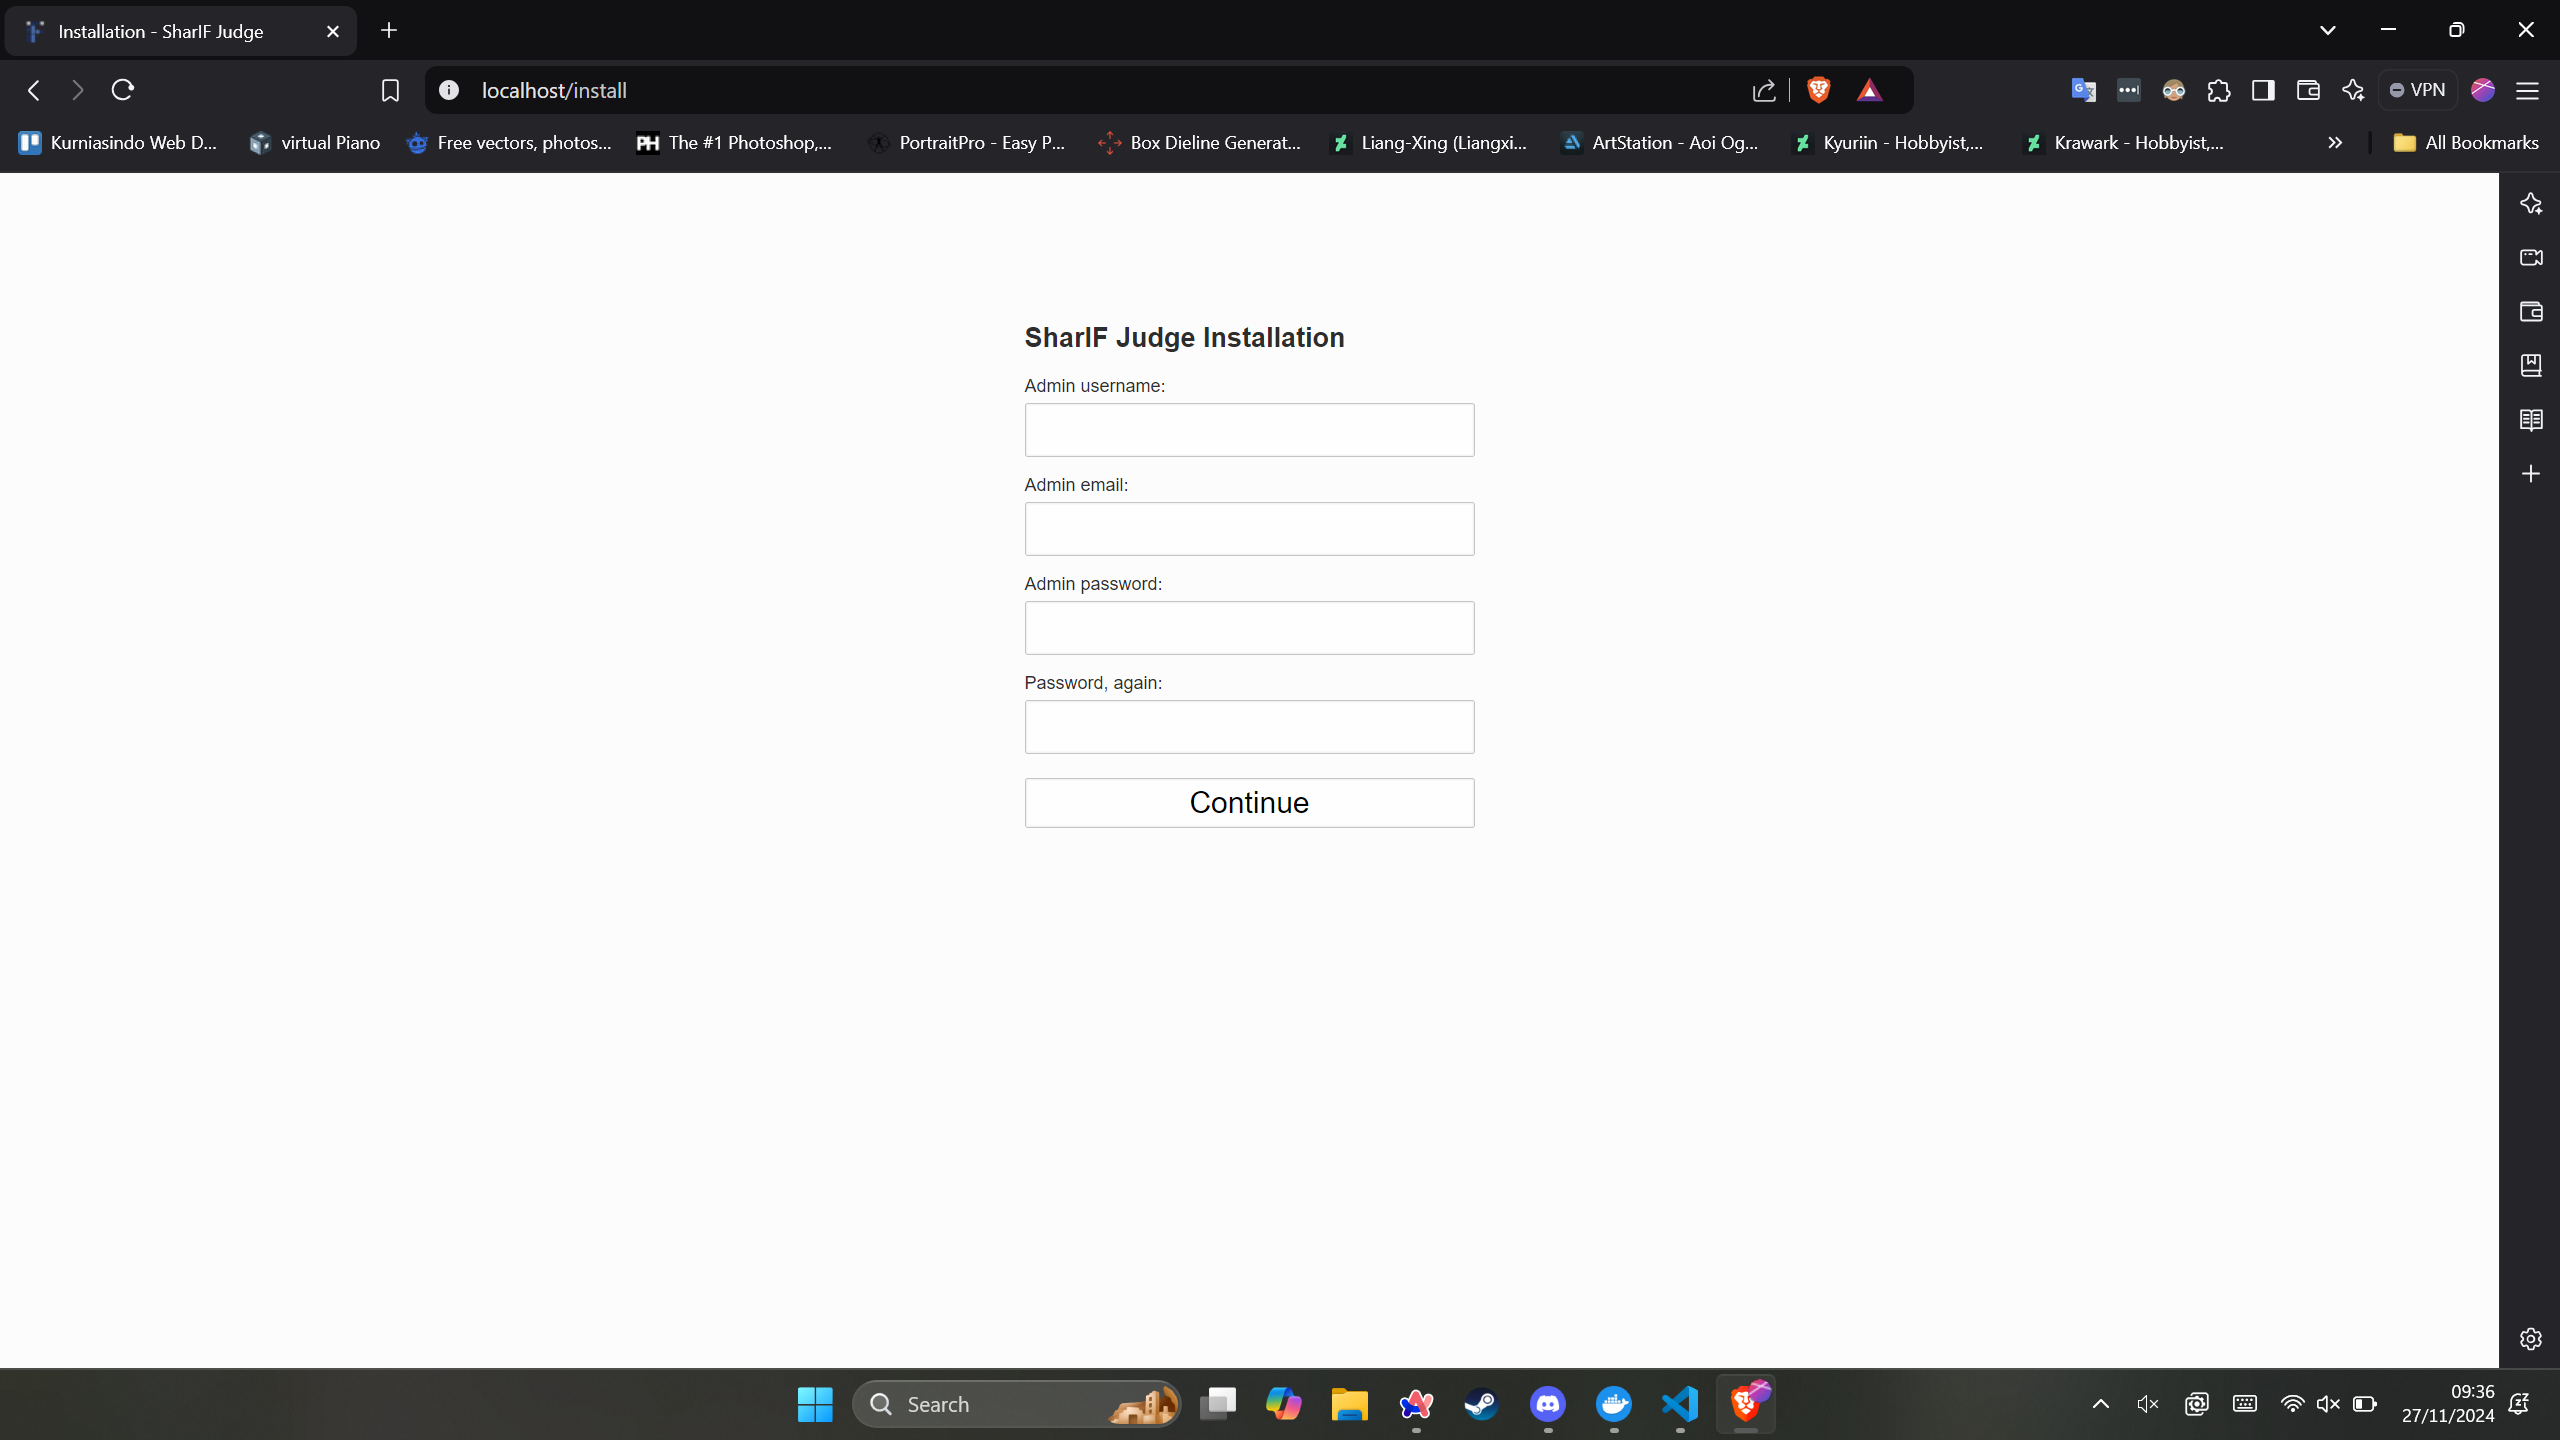
\includegraphics[width=0.7\textwidth]{views/install.png}
		      \caption{Halaman Install}
		      \label{fig:3:1:1:install}
	      \end{figure}


	\item \verb|Login.php| \\
	      Berikut fungsi dengan penjelasannya pada \textit{controller} \verb|Login.php|:

	      \begin{itemize}
		      \item \verb|index()| \\
		            Mengembalikan \textit{view} \verb|login.twig| dan memeriksa username dan password pada \textit{form} saat di kirim. Gambar \ref{fig:3:1:1:login} menunjukkan hasil halaman Login.

		            \begin{figure}[H]
			            \centering
			            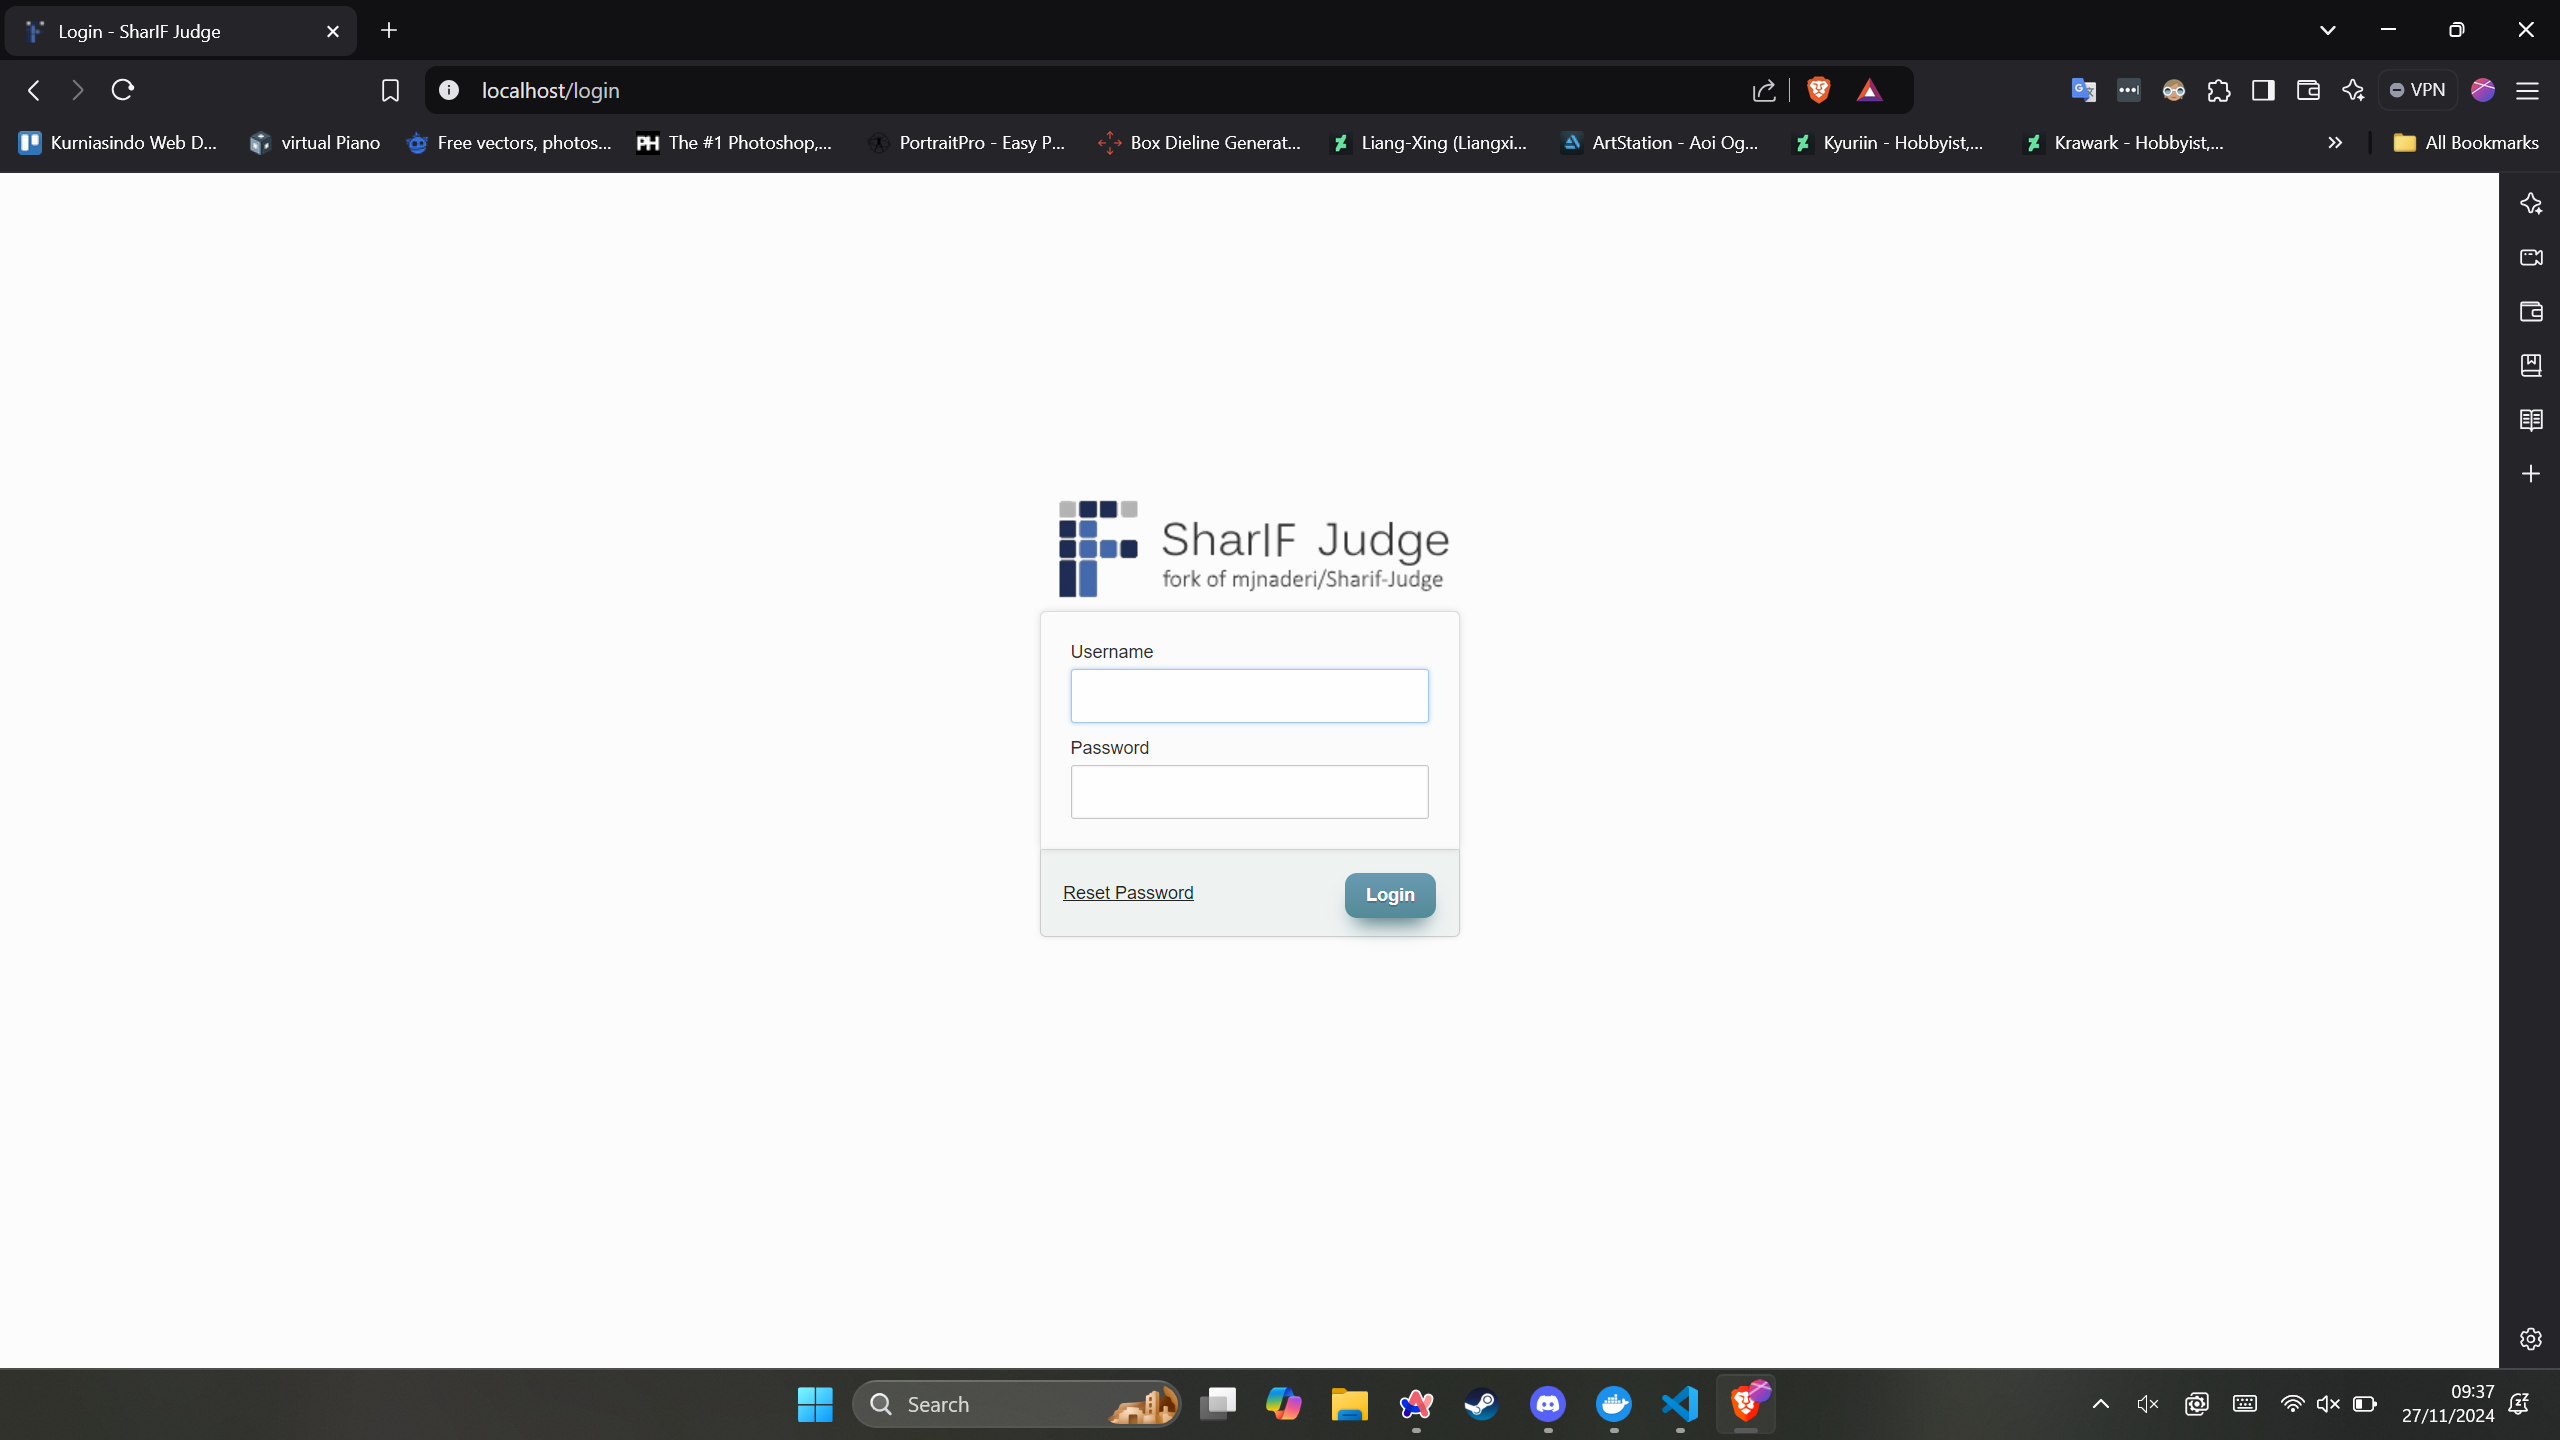
\includegraphics[width=0.7\textwidth]{views/login.png}
			            \caption{Halaman Login}
			            \label{fig:3:1:1:login}
		            \end{figure}
		      \item \verb|_registration_code($code)| \\
		            Melakukan validasi kode registrasi.
		      \item \verb|register()| \\
		            Menunjukkan halaman \verb|register.twig| dan membuat pengguna baru.
		      \item \verb|logout()| \\
		            Melakukan \textit{Log out} dan mengalihkan ke halaman \textit{login}.
		      \item \verb|lost()| \\
		            Mengirimkan email \textit{reset password}.
		      \item \verb|reset($passchange_key)| \\
		            Melakukan \textit{reset password} dengan halaman \verb|reset_password.twig|.

	      \end{itemize}

	\item \verb|Logs.php| \\
	      Pada \textit{controller} \verb|Logs.php| hanya memiliki satu fungsi yaitu \verb|index()|, dimana fungsi tersebut akan mendapatkan data dari \verb|Logs_model| dan menampilkan halaman \verb|logs.twig|. Gambar \ref{fig:3:1:1:log} menunjukkan halaman Log yang dinamakan halaman 24-Hour Log.

	      \begin{figure}[H]
		      \centering
		      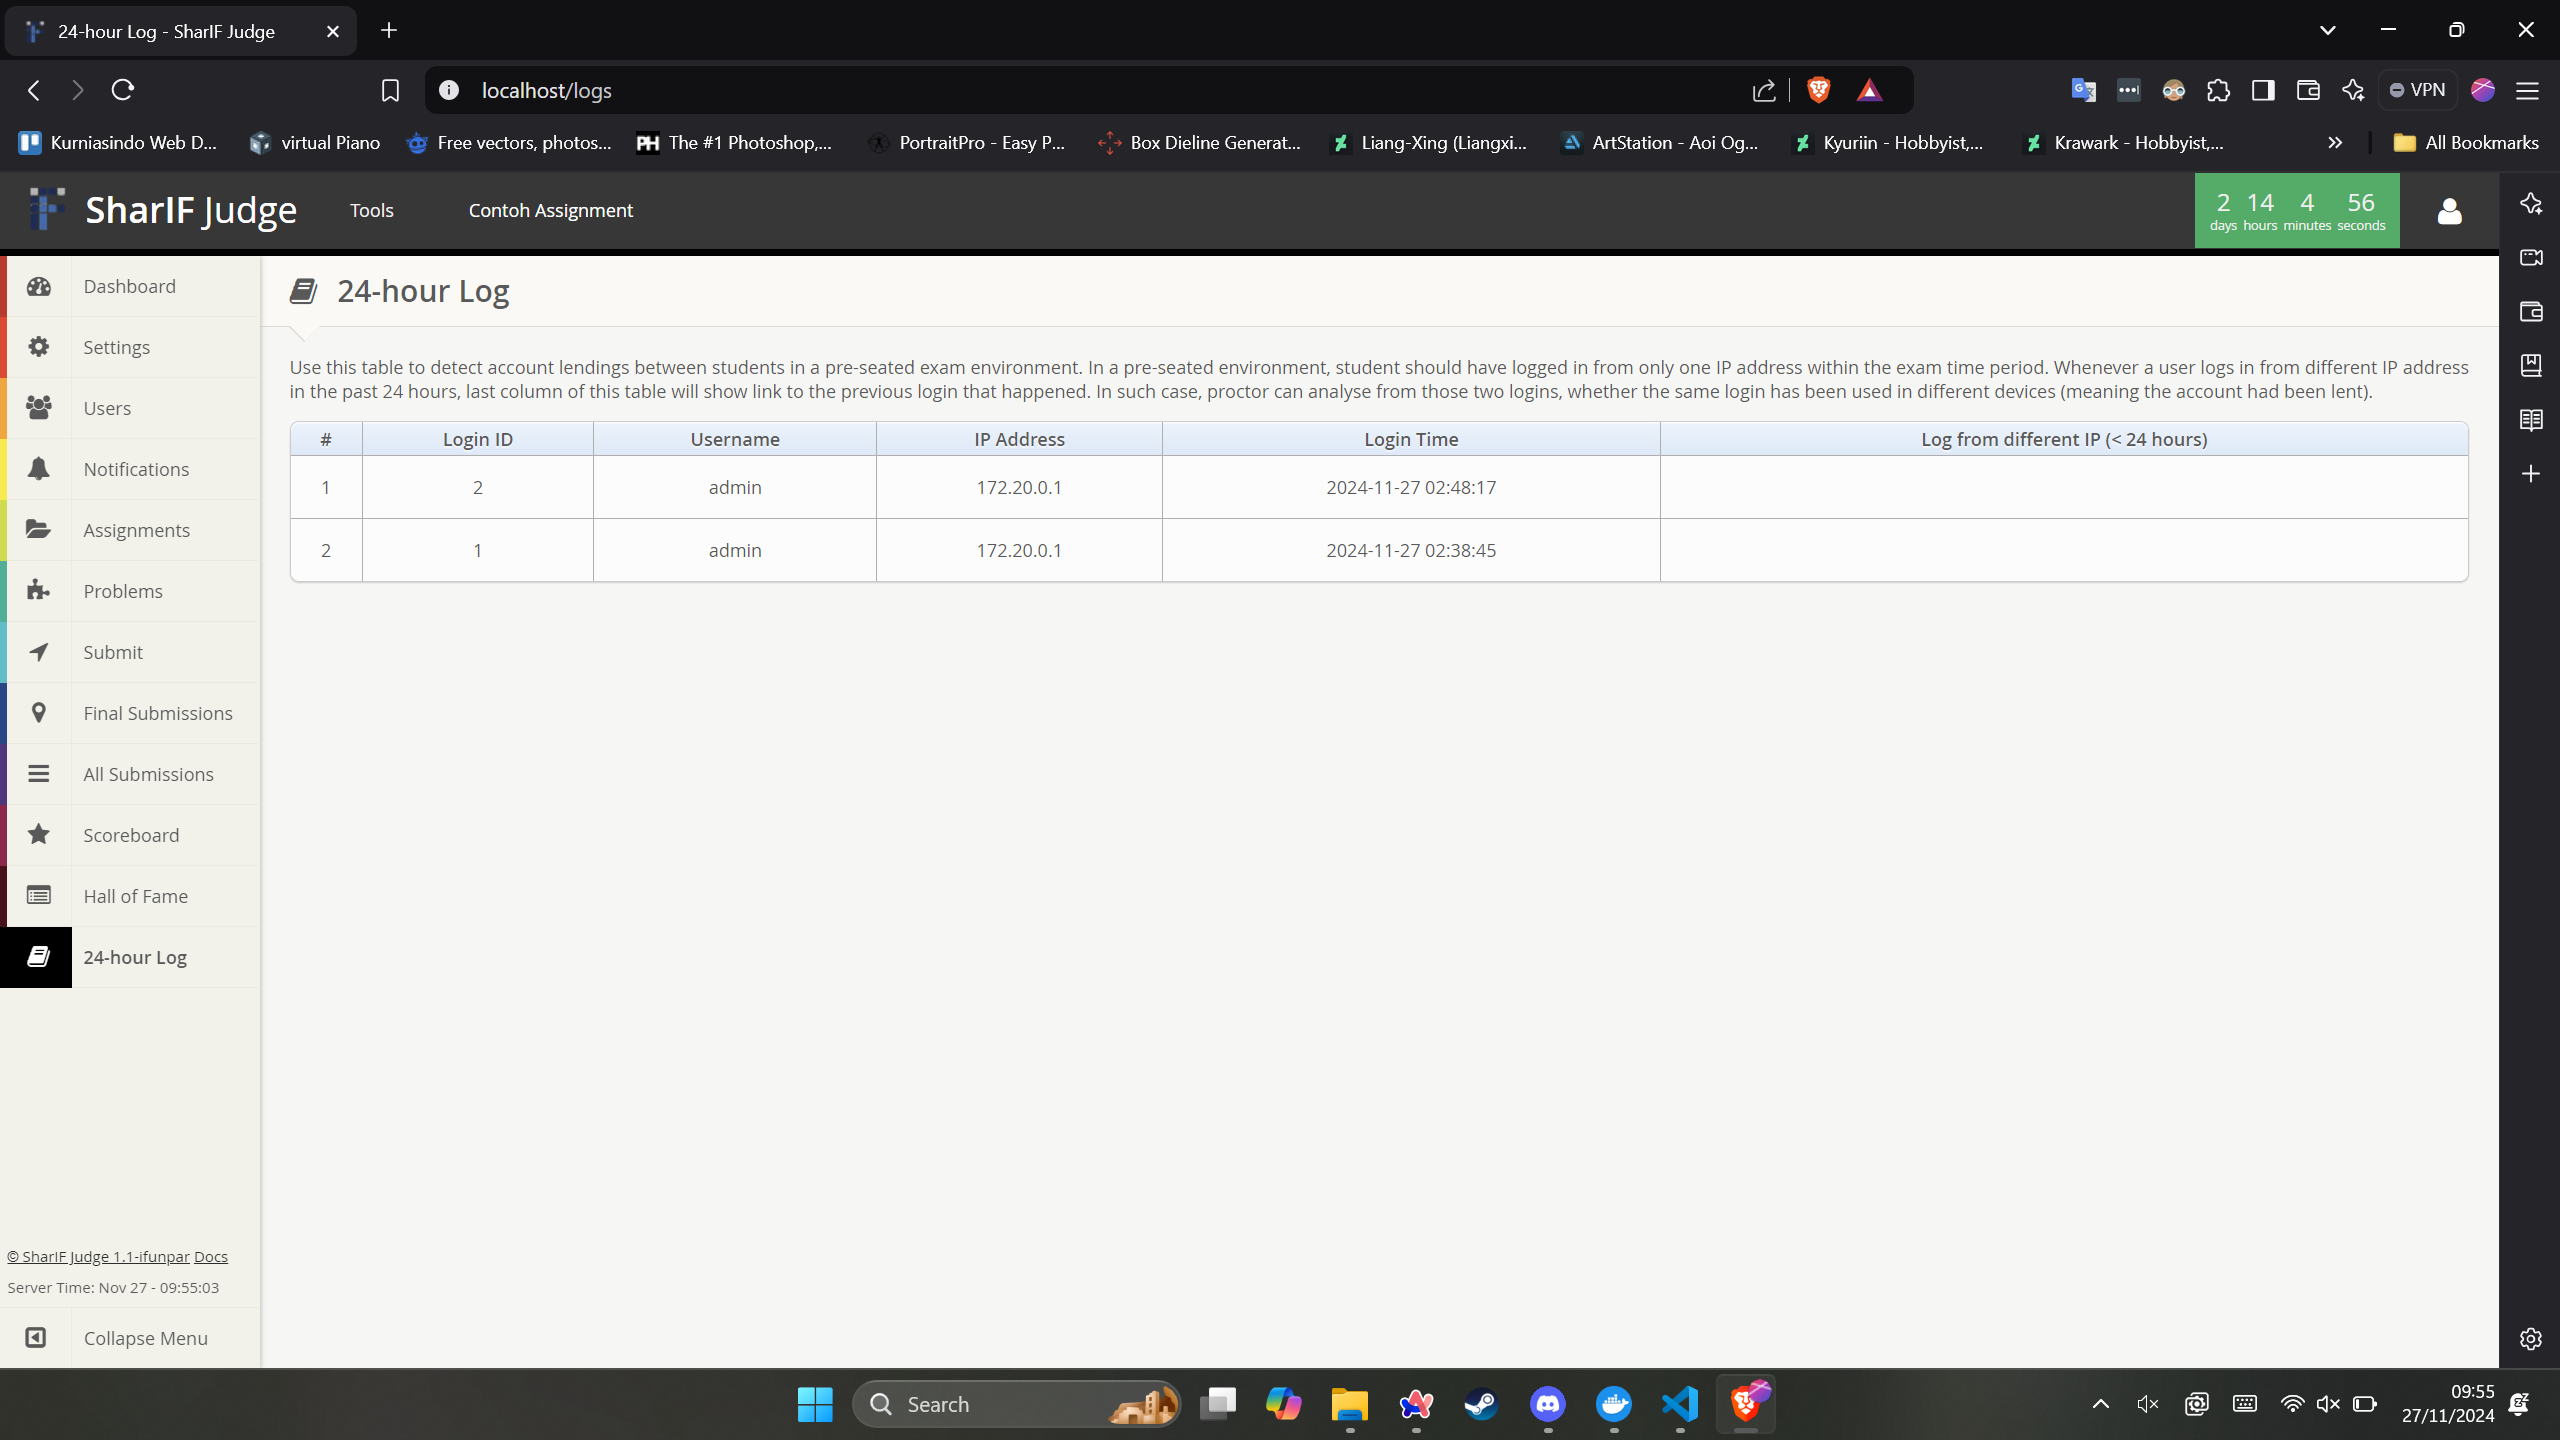
\includegraphics[width=0.7\textwidth]{views/log.png}
		      \caption{Halaman 24-Hour Log}
		      \label{fig:3:1:1:log}
	      \end{figure}


	\item \verb|Moss.php| \\
	      Berikut fungsi dengan penjelasannya pada \textit{controller} \verb|Moss.php|:

	      \begin{itemize}
		      \item \verb|index()| \\
		            Mengambil data dan memasukkannya ke dalam \textit{view} \verb|moss.twig|. Gambar \ref{fig:3:1:1:moss} merupakan hasil halaman moss. Fungsi \verb|_detect| juga akan dijalankan saat \textit{form} terkirim.

		            \begin{figure}[H]
			            \centering
			            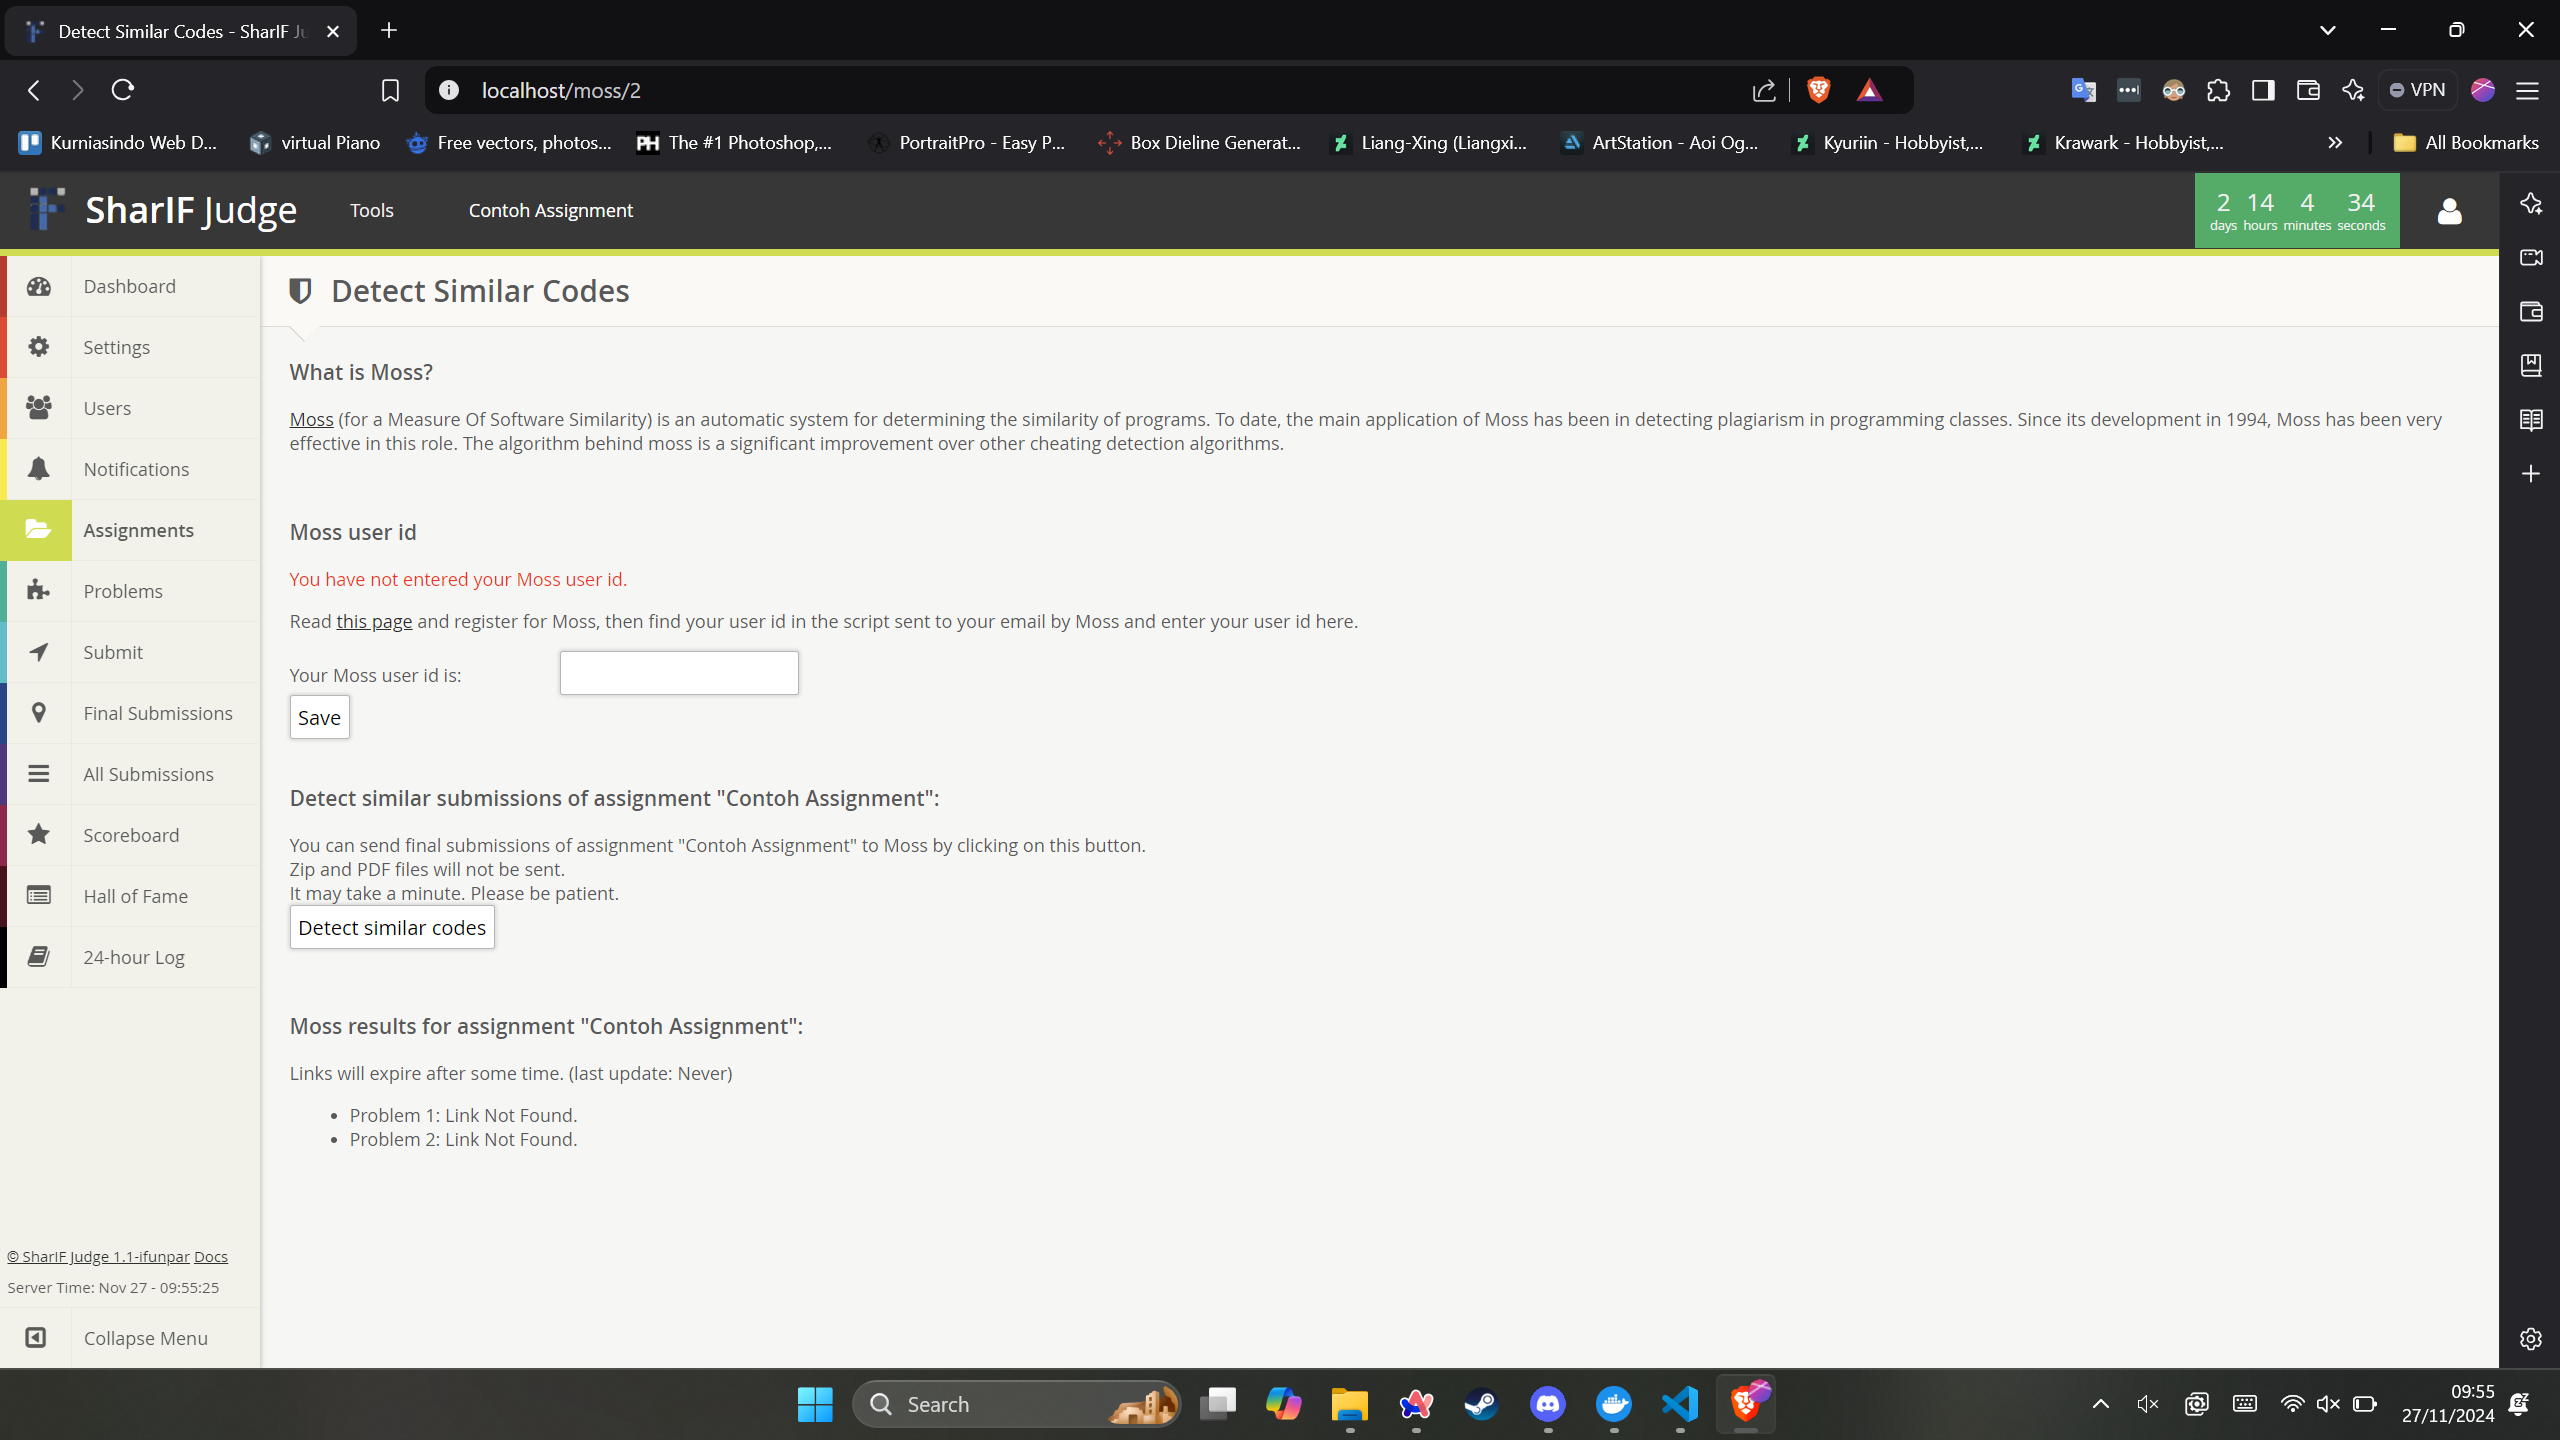
\includegraphics[width=0.7\textwidth]{views/moss.png}
			            \caption{Halaman Moss}
			            \label{fig:3:1:1:moss}
		            \end{figure}
		      \item \verb|update($assignment_id)| \\
		            Memperbaharui \textit{settings} dari masukkan \verb|moss_userid| pengguna.
		      \item \verb|_detect($assignment_id)| \\
		            Melakukan pemeriksaan kesamaan kode dengan Moss.

	      \end{itemize}

	\item \verb|Notifications.php| \\
	      Berikut fungsi dengan penjelasannya pada \textit{controller} \verb|Notifications.php|:

	      \begin{itemize}
		      \item \verb|add()| \\
		            Menambahkan atau memperbaharui sebuah \textit{notification}.
		      \item \verb|edit($notif_id)| \\
		            Menandai \textit{notification} yang akan di \textit{edit} dan memanggil fungsi \verb|add|.
		      \item \verb|delete()| \\
		            Menghapus sebuah \textit{notification}.
		      \item \verb|check()| \\
		            menggunakan \textit{ajax request} untuk mengetahui ketersediaan \textit{notification} baru.
		      \item \verb|index()| \\
		            Mendapatkan data dari dua model yaitu \verb|Assignment_model| dan \verb|Notifications_model|. Data akan dimasukkan ke dalam \textit{view} \verb|notifications.twig| yang akan dikembalikan ke pengguna. Gambar \ref{fig:3:1:1:notif} menunjukkan hasil halaman \textit{Notifications}.

		            \begin{figure}[H]
			            \centering
			            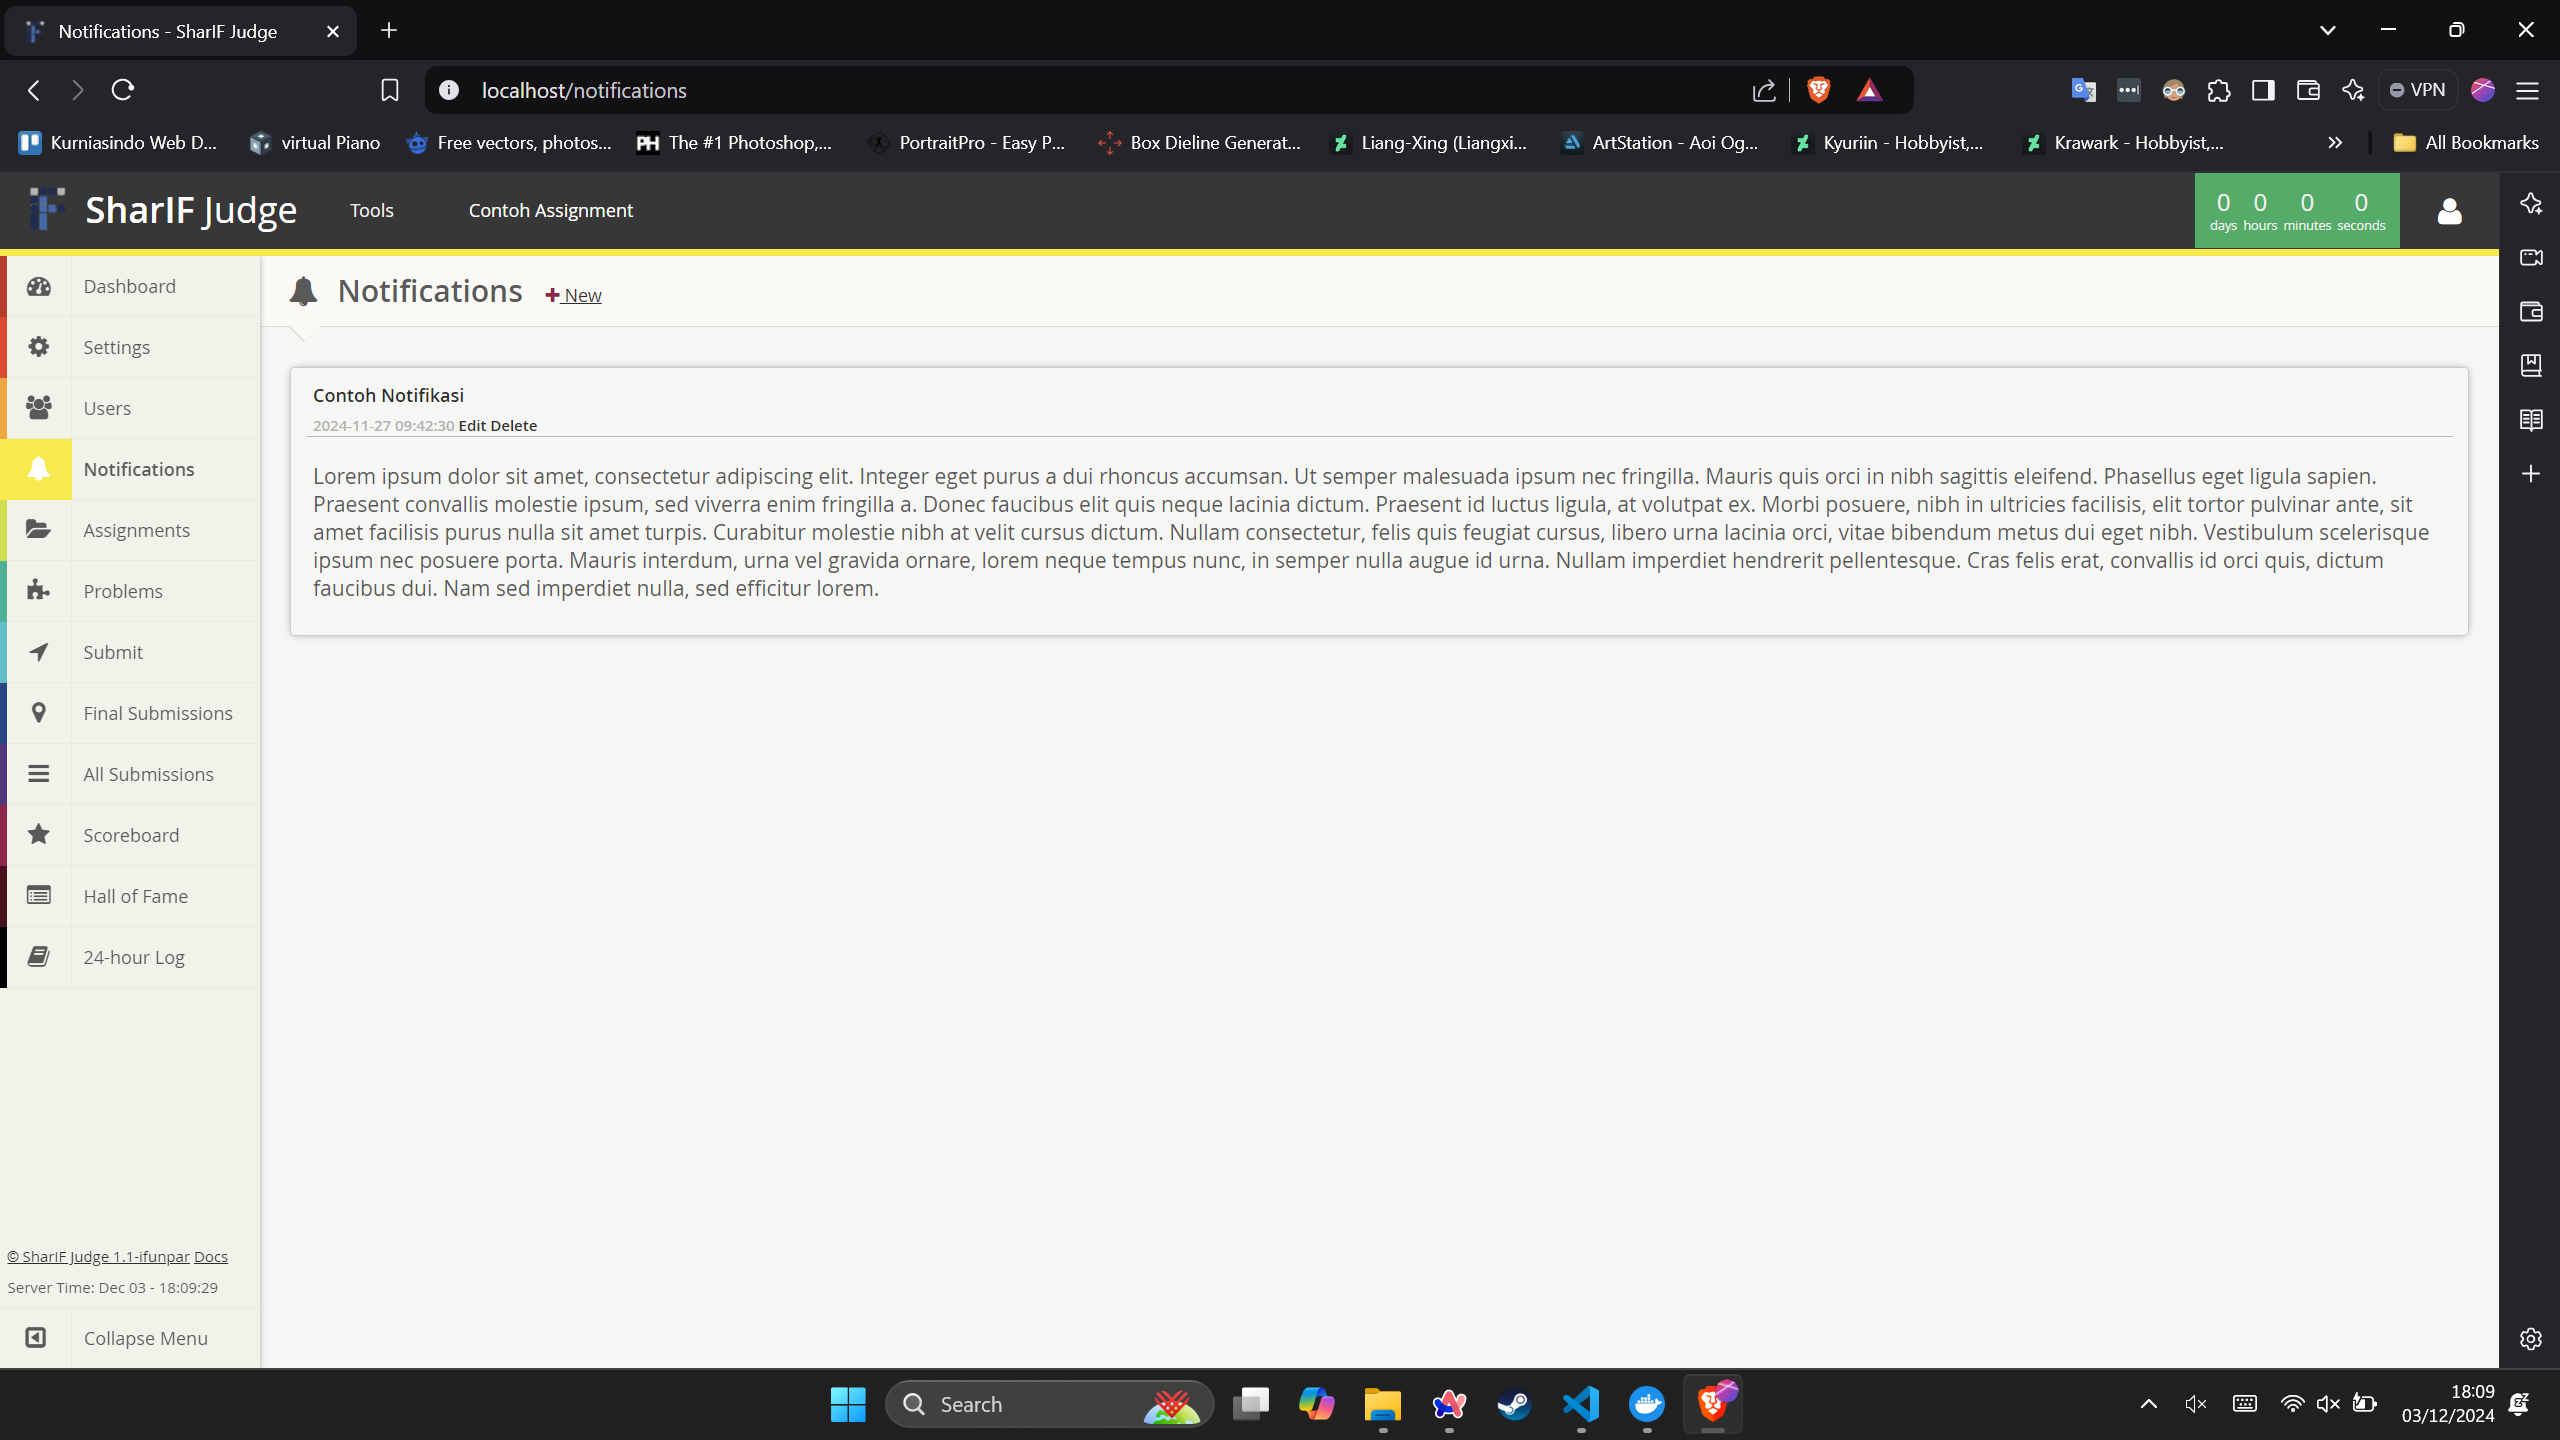
\includegraphics[width=0.75\textwidth]{views/notifications.png}
			            \caption{Halaman Notifications}
			            \label{fig:3:1:1:notif}
		            \end{figure}

	      \end{itemize}

	\item \verb|Problems.php| \\
	      Berikut fungsi dengan penjelasannya pada \textit{controller} \verb|Notifications.php|:

	      \begin{itemize}
		      \item \verb|edit()| \\
		            Memperbaharui deskripsi sebuah \textit{problem} dalam bentuk \verb|html| atau \verb|markdown|.
		      \item \verb|index()| \\
		            Mendapatkan data \textit{problem} dari berbagai \textit{model} sesuai dengan \textit{assignment} yang dipilih dan menyimpan data tersebut pada halaman \verb|problems.twig| yang akan ditampilkan ke pengguna. Gambar \ref{fig:3:1:1:problem} menunjukkan hasil halaman Problems.

		            \begin{figure}[H]
			            \centering
			            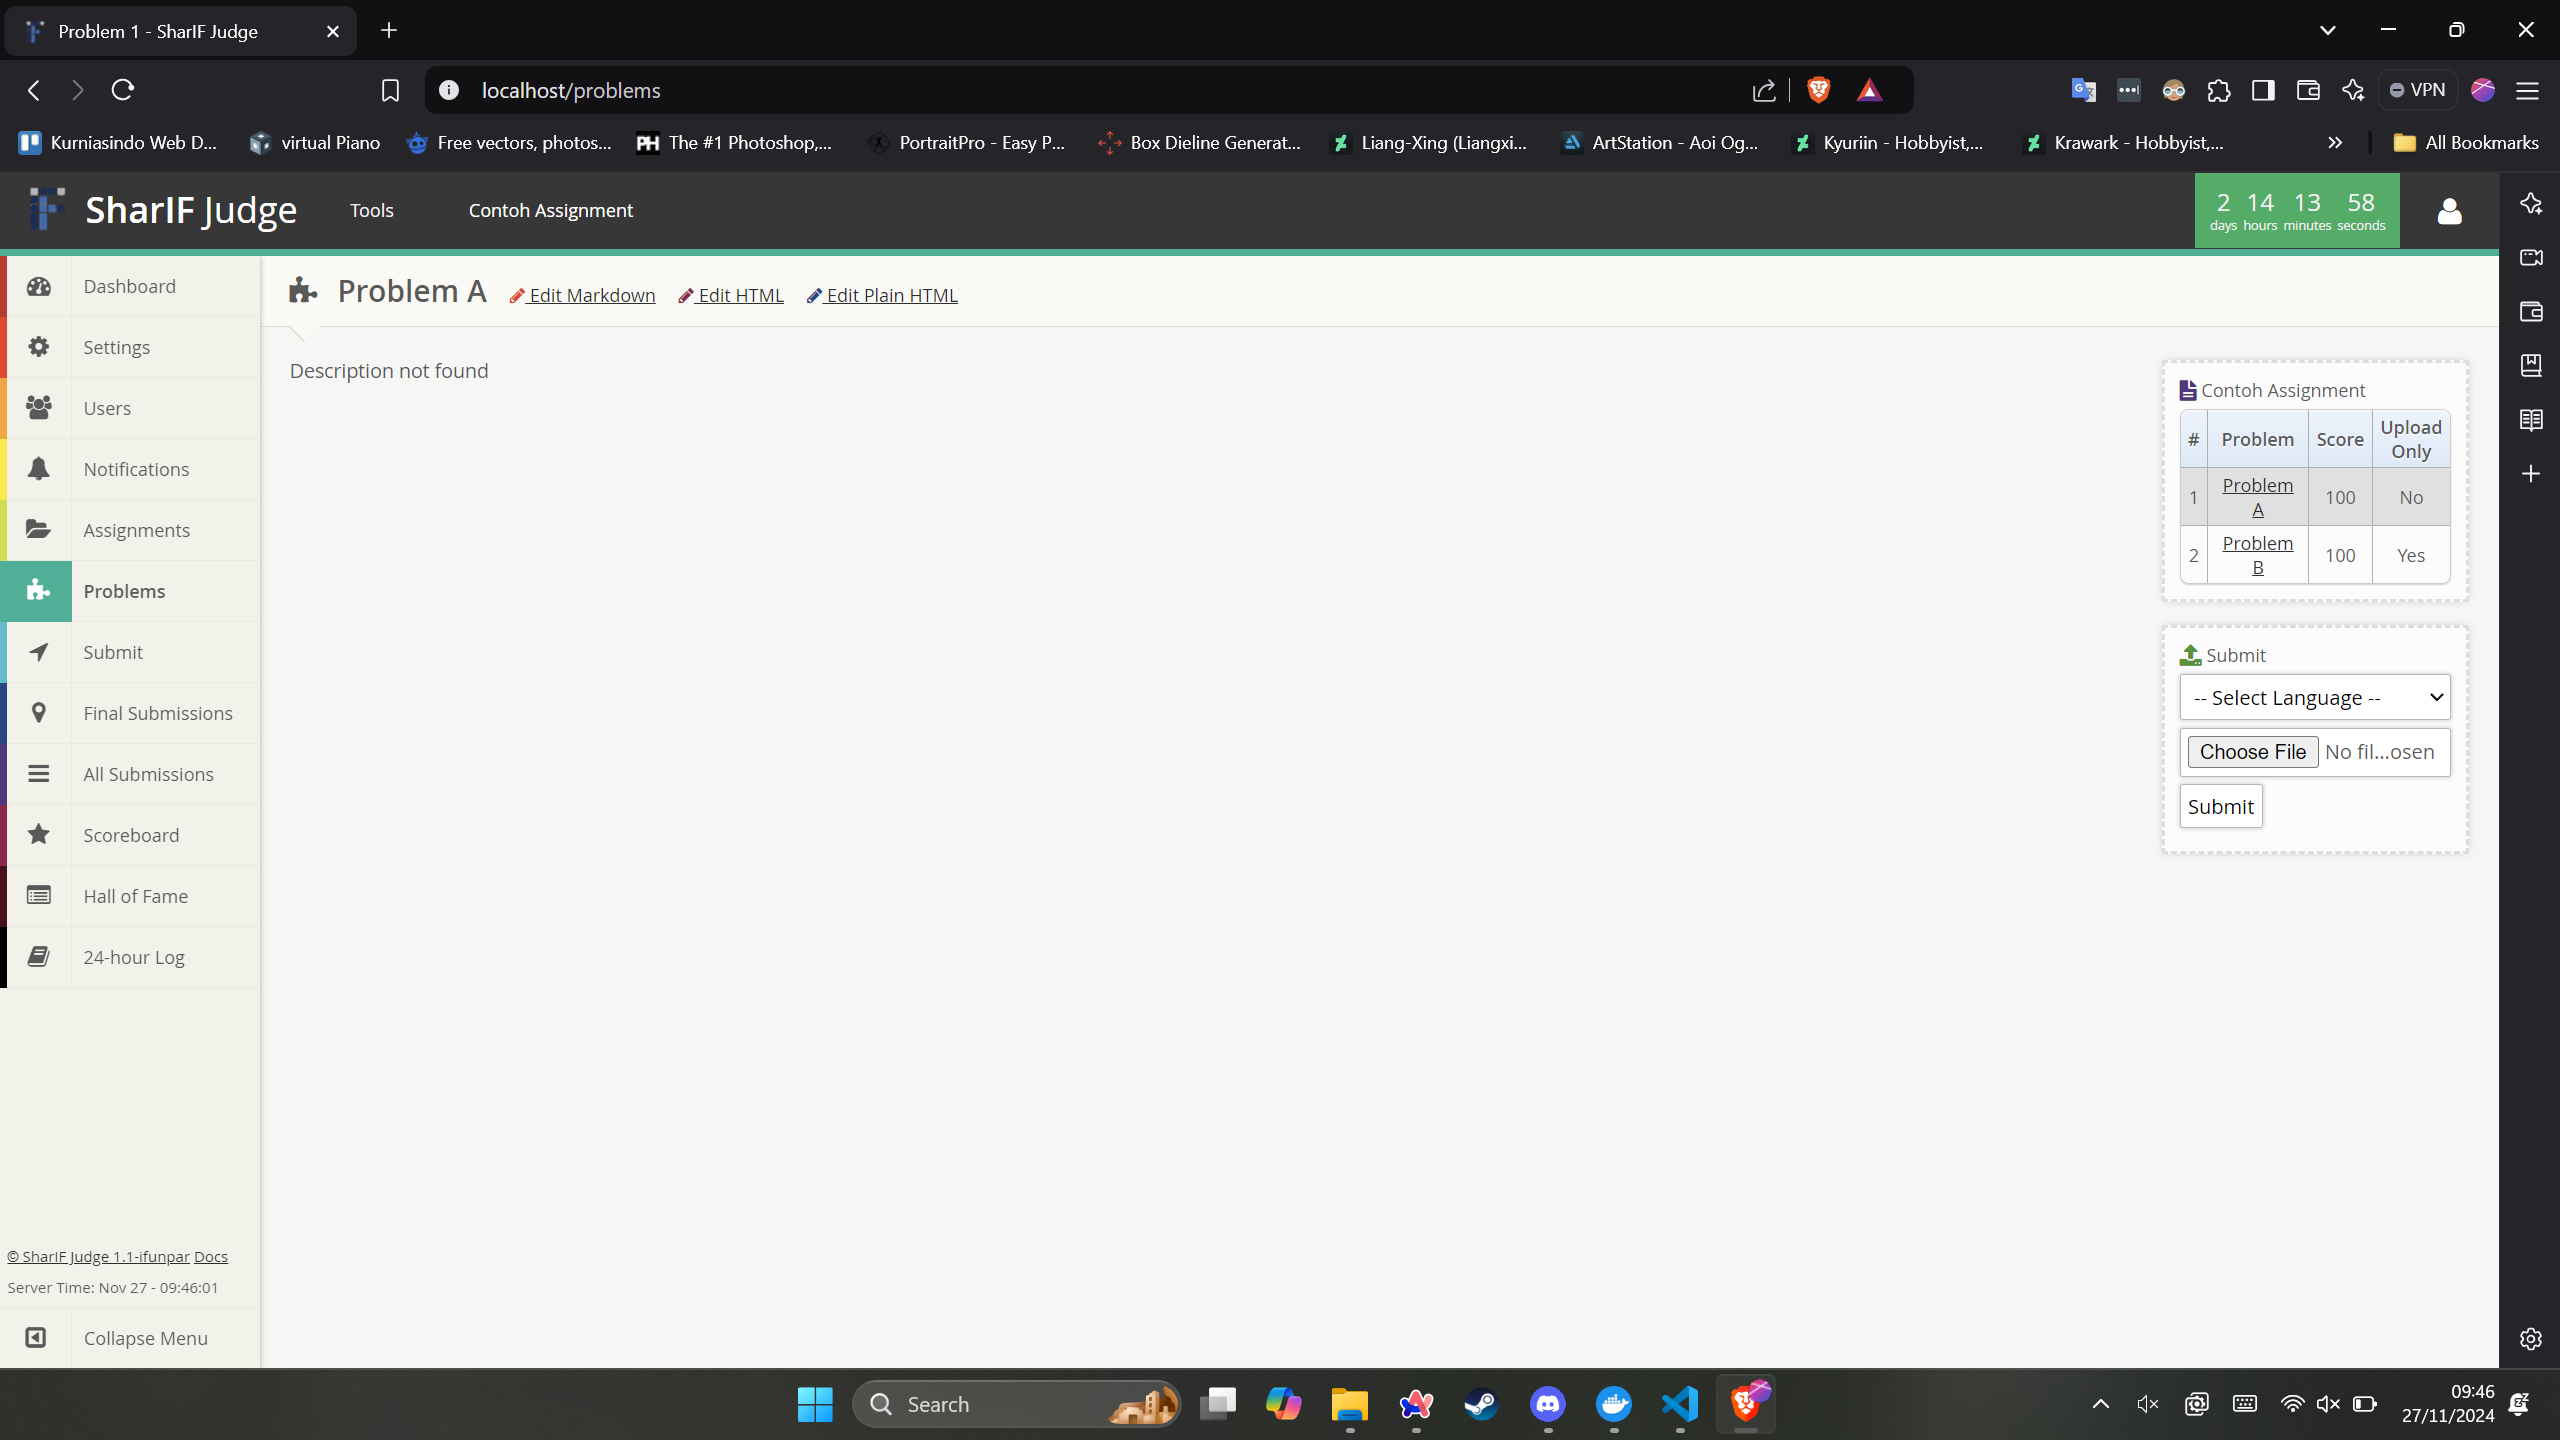
\includegraphics[width=0.75\textwidth]{views/problem.png}
			            \caption{Halaman Problems}
			            \label{fig:3:1:1:problem}
		            \end{figure}

	      \end{itemize}

	\item \verb|Profile.php| \\
	      Berikut fungsi dengan penjelasannya pada \textit{controller} \verb|Profile.php|:

	      \begin{itemize}
		      \item \verb|index()| \\
		            Mendapatkan data dari berbagai \textit{model} terutama dari pengguna yang akan dimasukkan ke dalam \textit{view} \verb|profile.twig|. Fungsi ini juga menangani pengiriman \textit{form} pembaharuan data pengguna pengguna. Gambar \ref{fig:3:1:1:profile} menunjukkan hasil halaman Profile.

		            \begin{figure}[H]
			            \centering
			            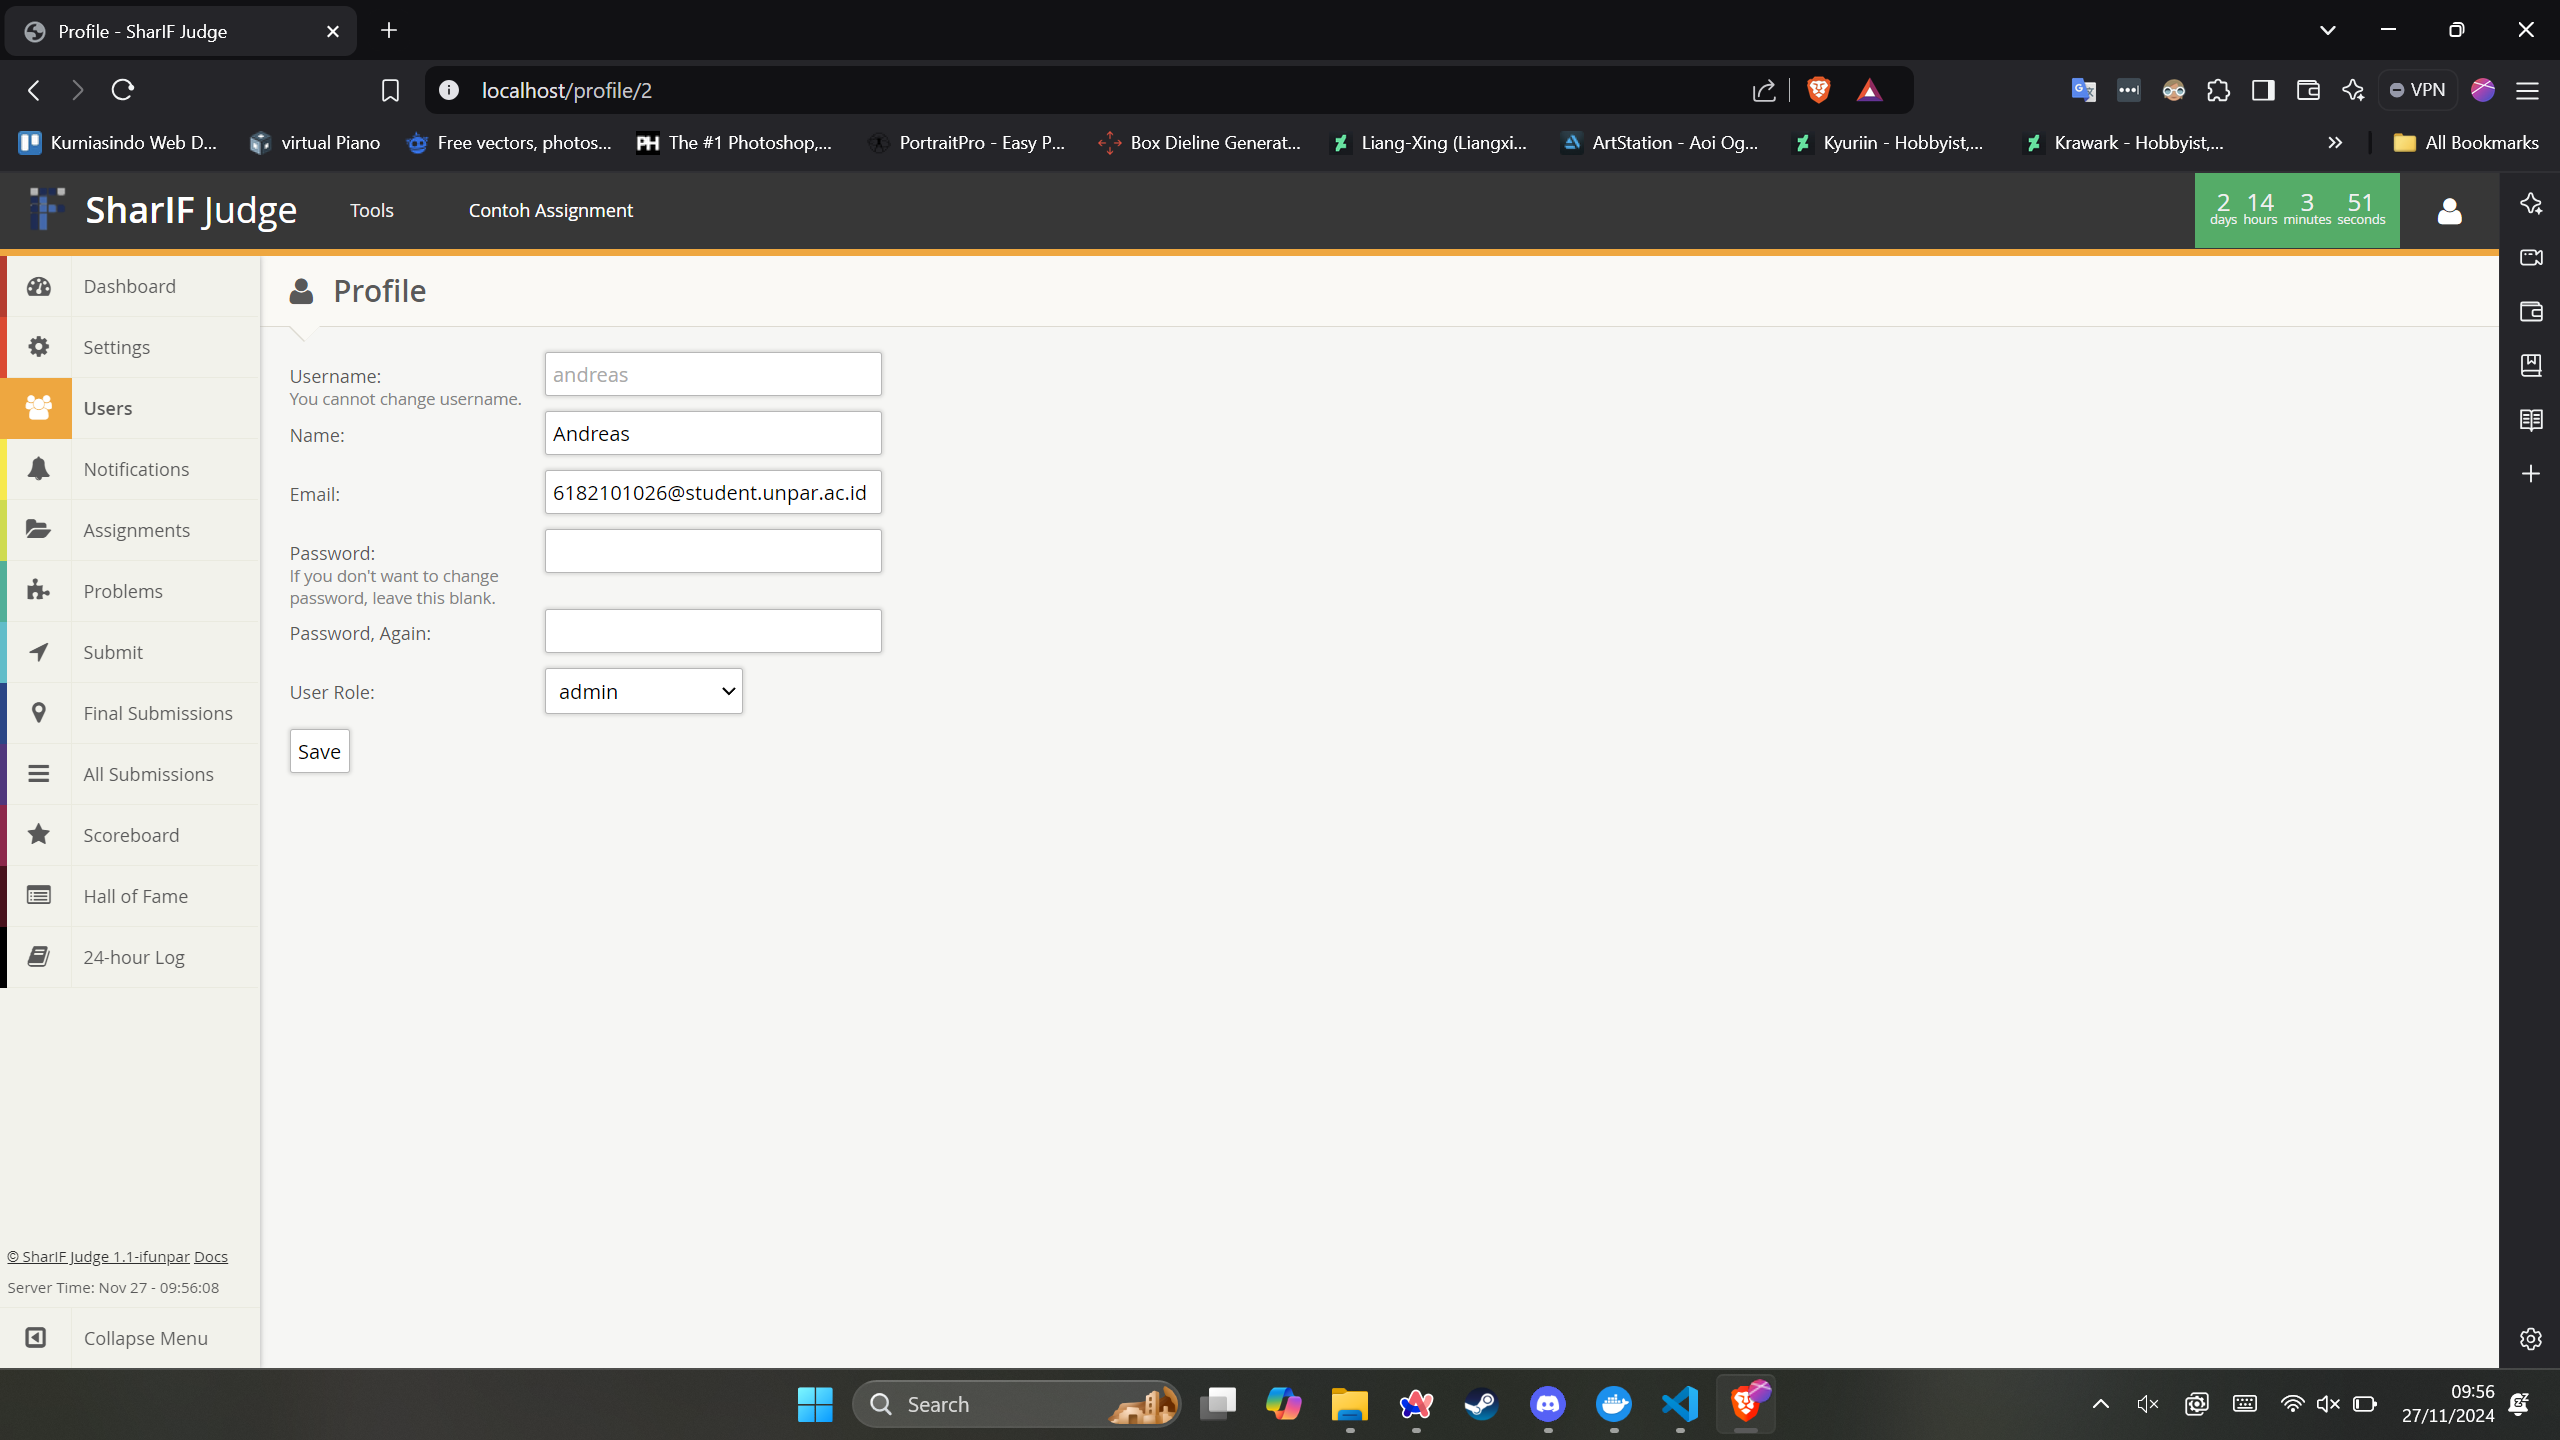
\includegraphics[width=0.9\textwidth]{views/profile.png}
			            \caption{Halaman Profile}
			            \label{fig:3:1:1:profile}
		            \end{figure}
		      \item \verb|_password_check($str)| \\
		            Melakukan validasi \textit{input password}.
		      \item \verb|_password_again_check($str)| \\
		            Melakukan validasi \textit{input} tulisan pengulangan \textit{password}.
		      \item \verb|_email_check($str)| \\
		            Melakukan validasi ketersediaan email pada \textit{database}.
		      \item \verb|_role_check($str)| \\
		            Melakukan validasi \textit{role} pengguna saat ingin mengubah \textit{role} pengguna.

	      \end{itemize}

	\item \verb|Queue.php| \\
	      Berikut fungsi dengan penjelasannya pada \textit{controller} \verb|Profile.php|:

	      \begin{itemize}
		      \item \verb|pause()| \\
		            Memberhentikan proses \textit{queue}.
		      \item \verb|resume()| \\
		            Melanjutkan proses \textit{queue}.
		      \item \verb|empty_queue()| \\
		            Menghapus semua \textit{queue} yang ada.
		      \item \verb|index()| \\
		            Mendapatkan data dari \textit{model} \verb|Queue|, \verb|Assignments_model|, dan \verb|Settings_model| yang dipakai dalam \textit{view} \verb|queue.twig| dan ditampilkan kepada pengguna. Gambar \ref{fig:3:1:1:queue} menunjukkan hasil halaman Queue.

		            \begin{figure}
			            \centering
			            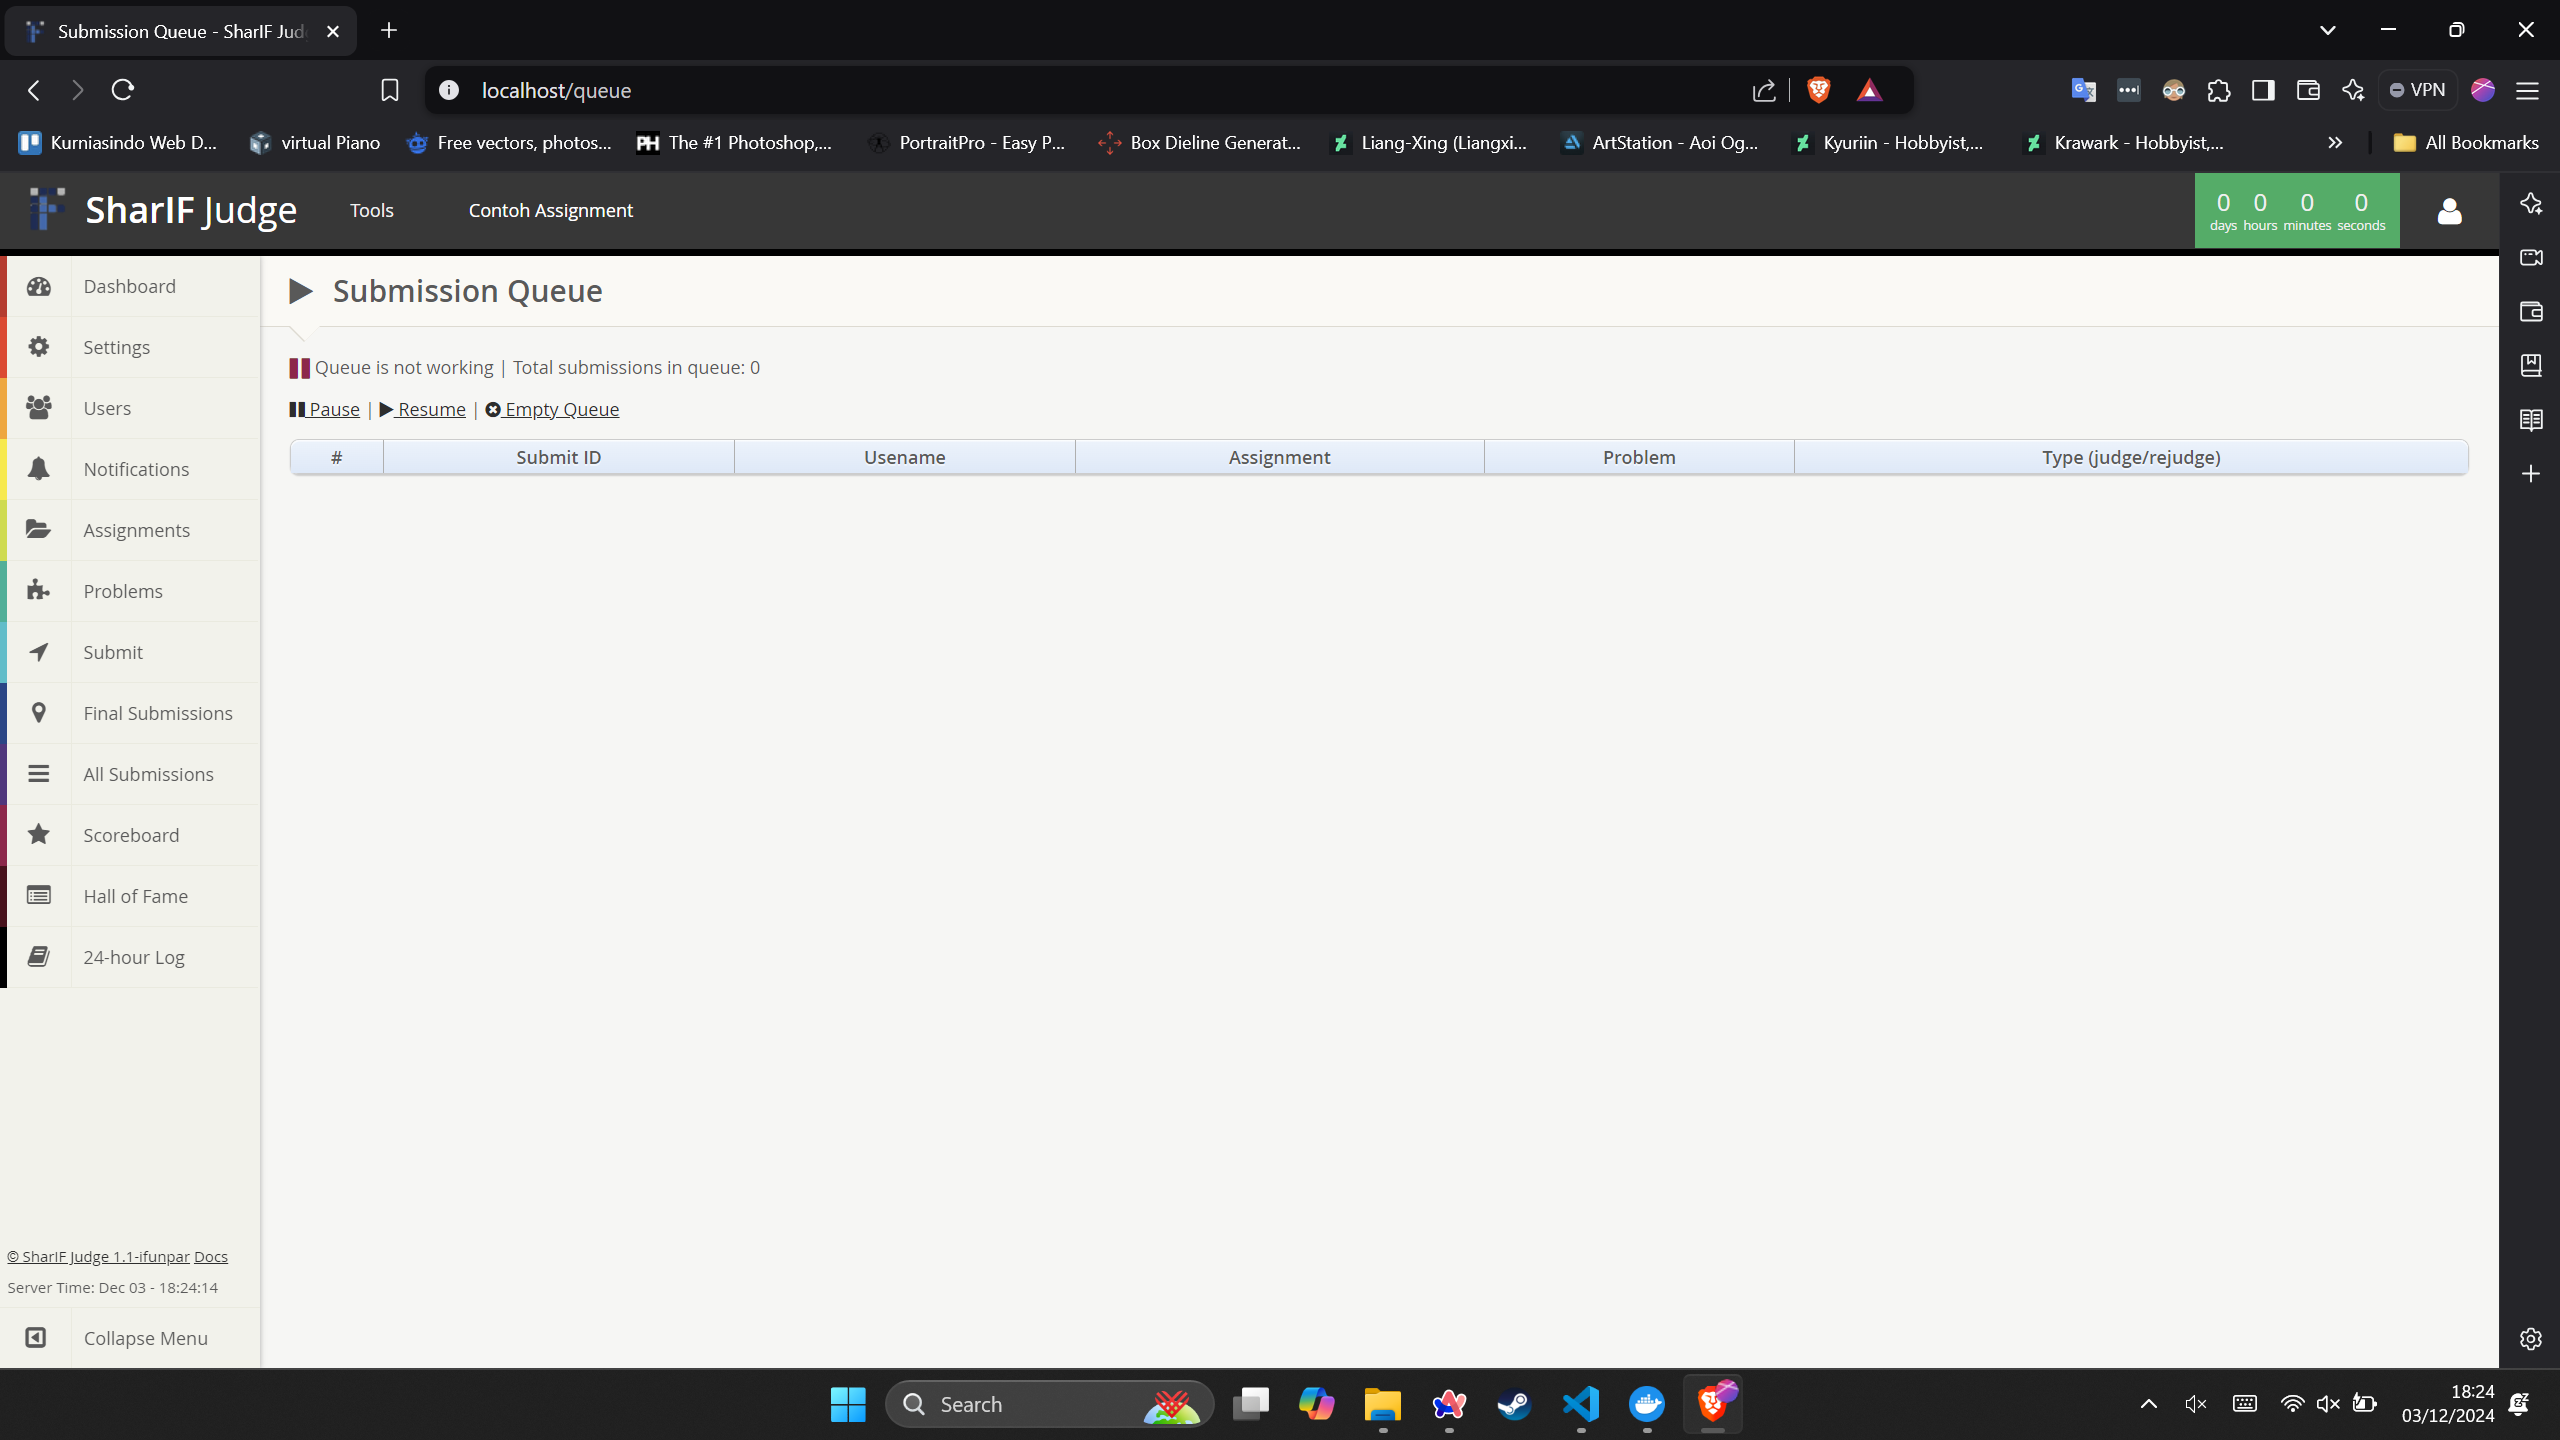
\includegraphics[width=0.875\textwidth]{views/queue.png}
			            \caption{Halaman Queue}
			            \label{fig:3:1:1:queue}
		            \end{figure}

	      \end{itemize}

	\item \verb|Queueprocess.php| \\
	      \textit{Controller} \verb|Queueprocess.php| hanya memiliki satu fungsi yaitu \verb|run()| yang akan menjalankan \textit{queue} satu per satu menggunakan \verb|bash|.

	      \newpage

	\item \verb|Rejudge.php| \\
	      Berikut fungsi dengan penjelasannya pada \textit{controller} \verb|Profile.php|:

	      \begin{itemize}
		      \item \verb|rejudge_single()| \\
		            Melakukan \textit{rejudge} untuk satu buah \textit{submission}.
		      \item \verb|index()| \\
		            Mendapatkan data dan menampilkan \verb|rejudge.twig|. Fungsi ini juga dapat melakukan \textit{rejudge} pada sebuah \textit{problem} tertentu. Gambar \ref{fig:3:1:1:rejudge} menunjukkan halaman Rejudge.

		            \begin{figure}[h]
			            \centering
			            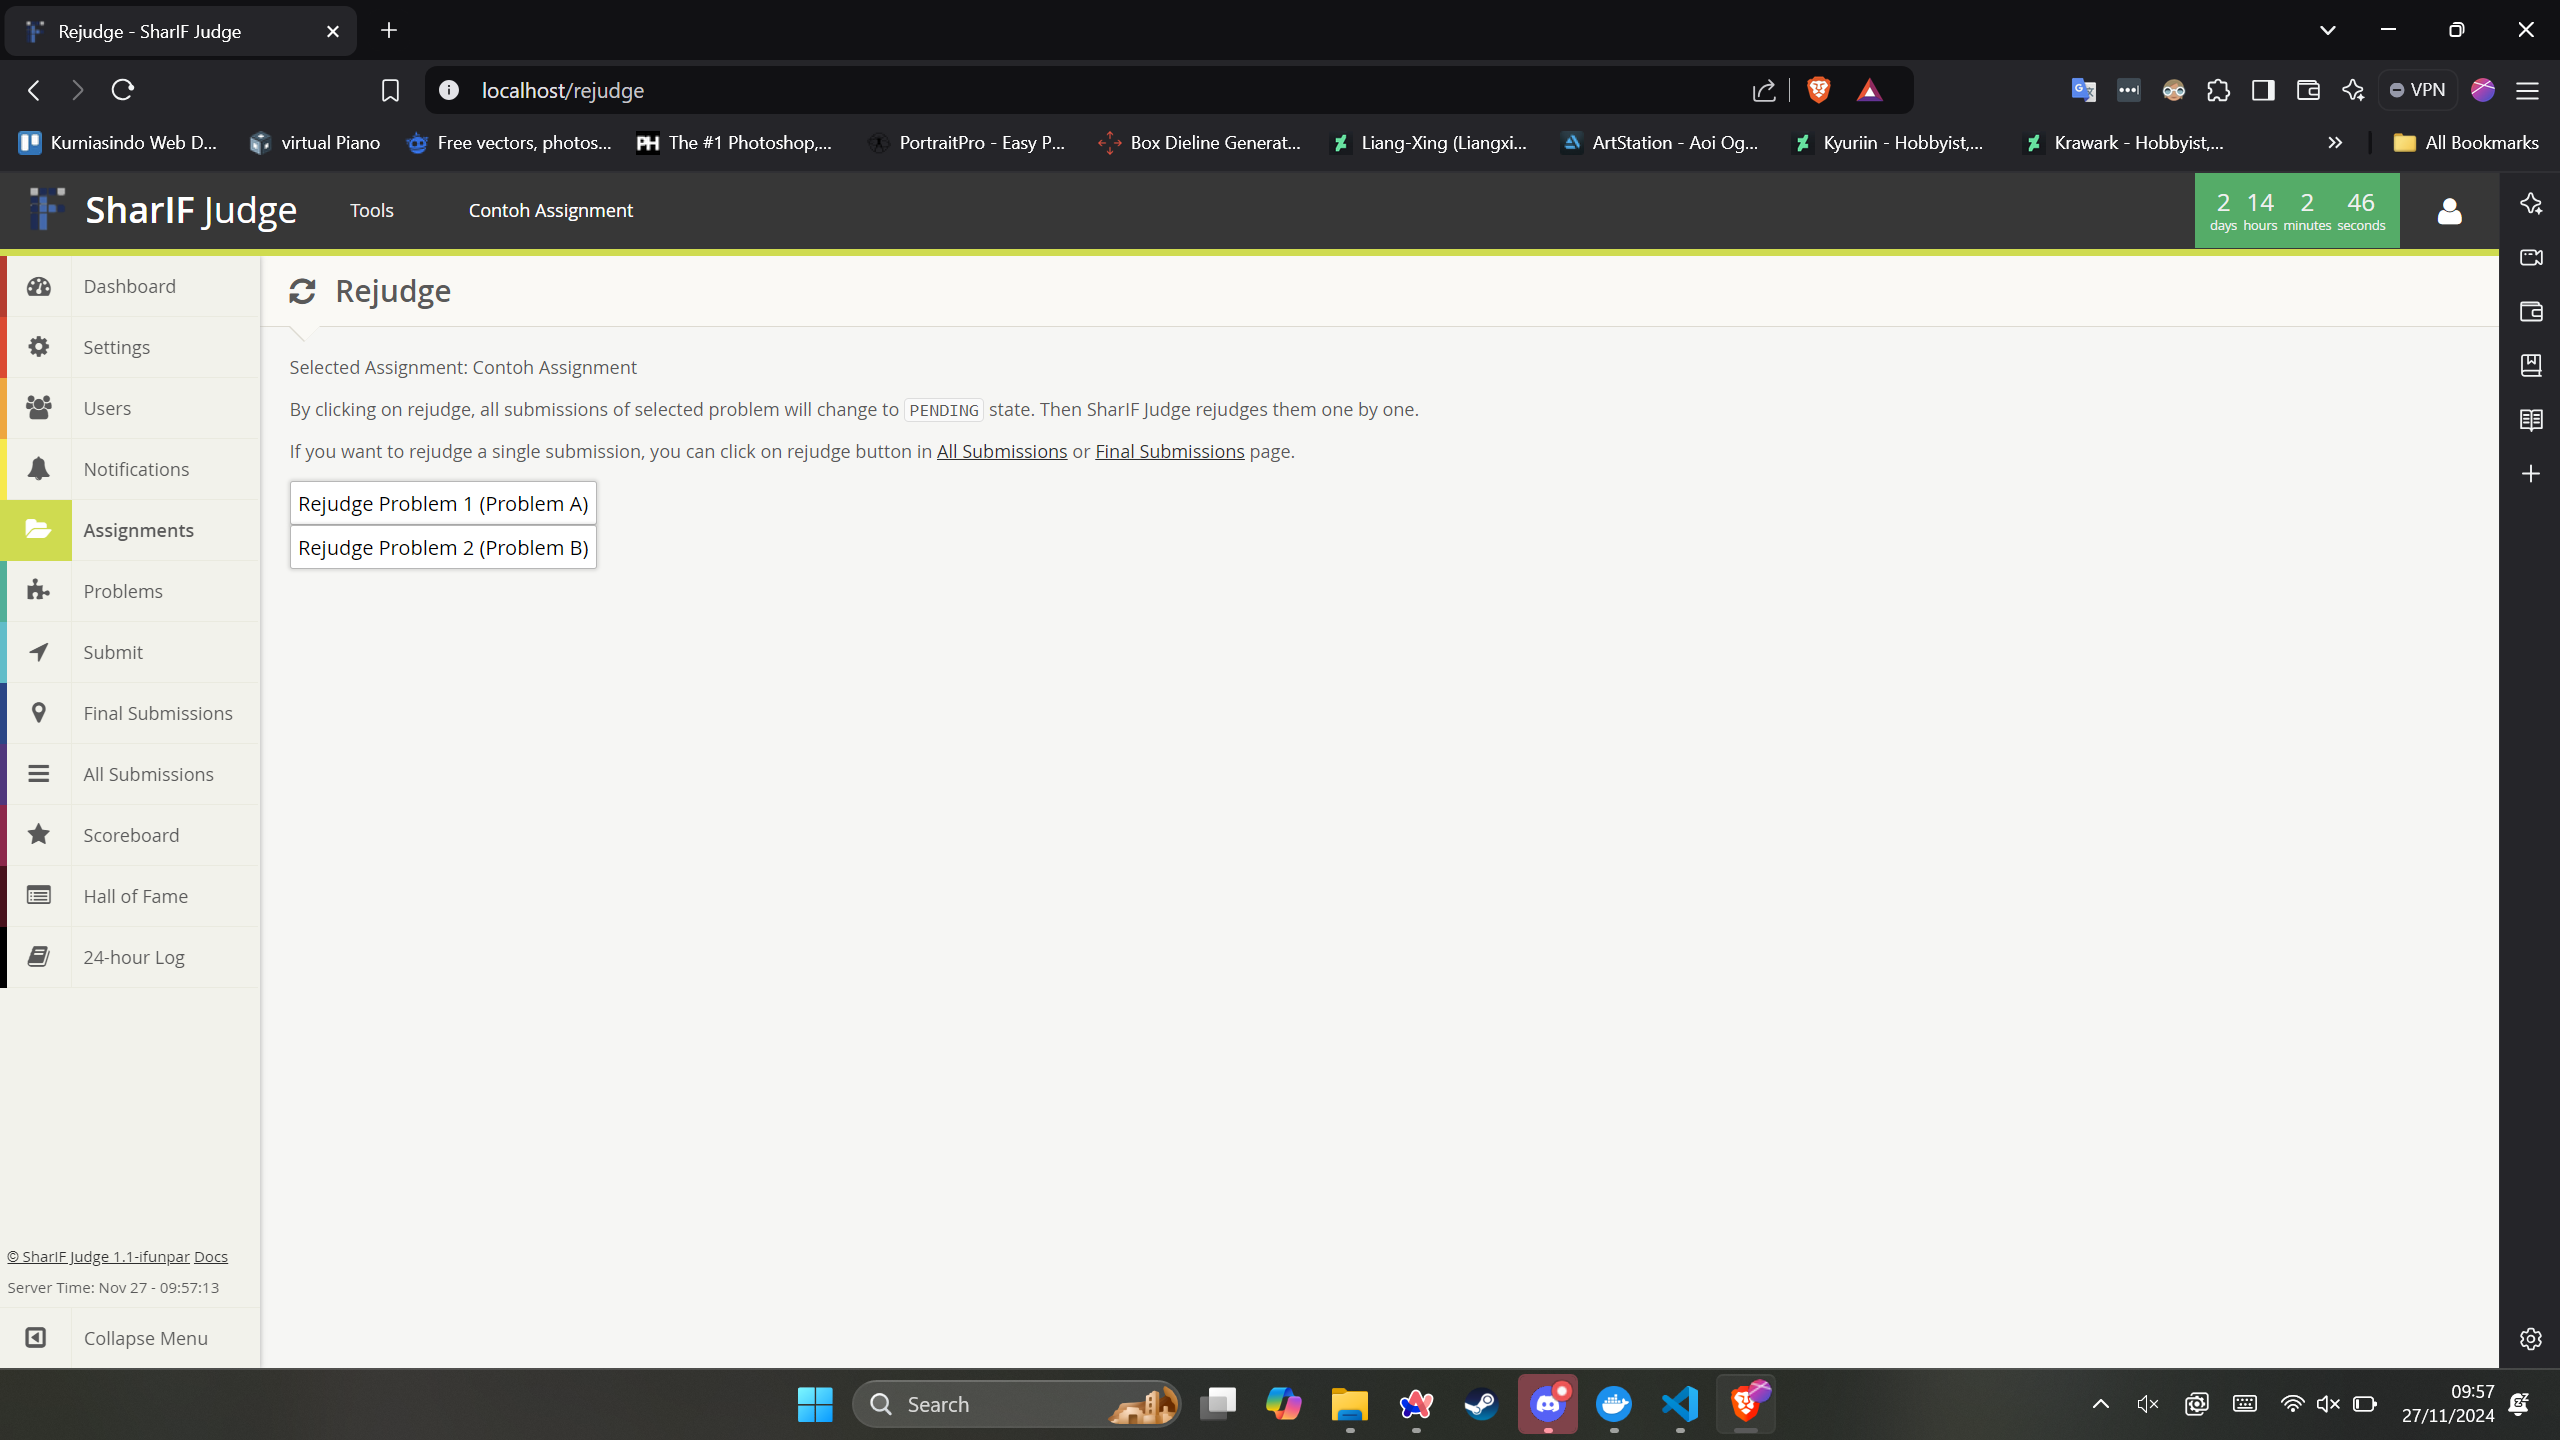
\includegraphics[width=0.875\textwidth]{views/rejudge.png}
			            \caption{Halaman Rejudge}
			            \label{fig:3:1:1:rejudge}
		            \end{figure}

	      \end{itemize}

	\item \verb|Scoreboard.php| \\
	      \textit{Controller} \verb|Queueprocess.php| hanya memiliki satu fungsi yaitu \verb|index()| yang akan menampilkan \textit{view} \verb|scoreboard.twig| dengan data yang didapat dari model \verb|Scoreboard_model|. Gambar \ref{fig:3:1:1:scoreboard} menunjukkan hasil halaman Scoreboard.

	      \begin{figure}
		      \centering
		      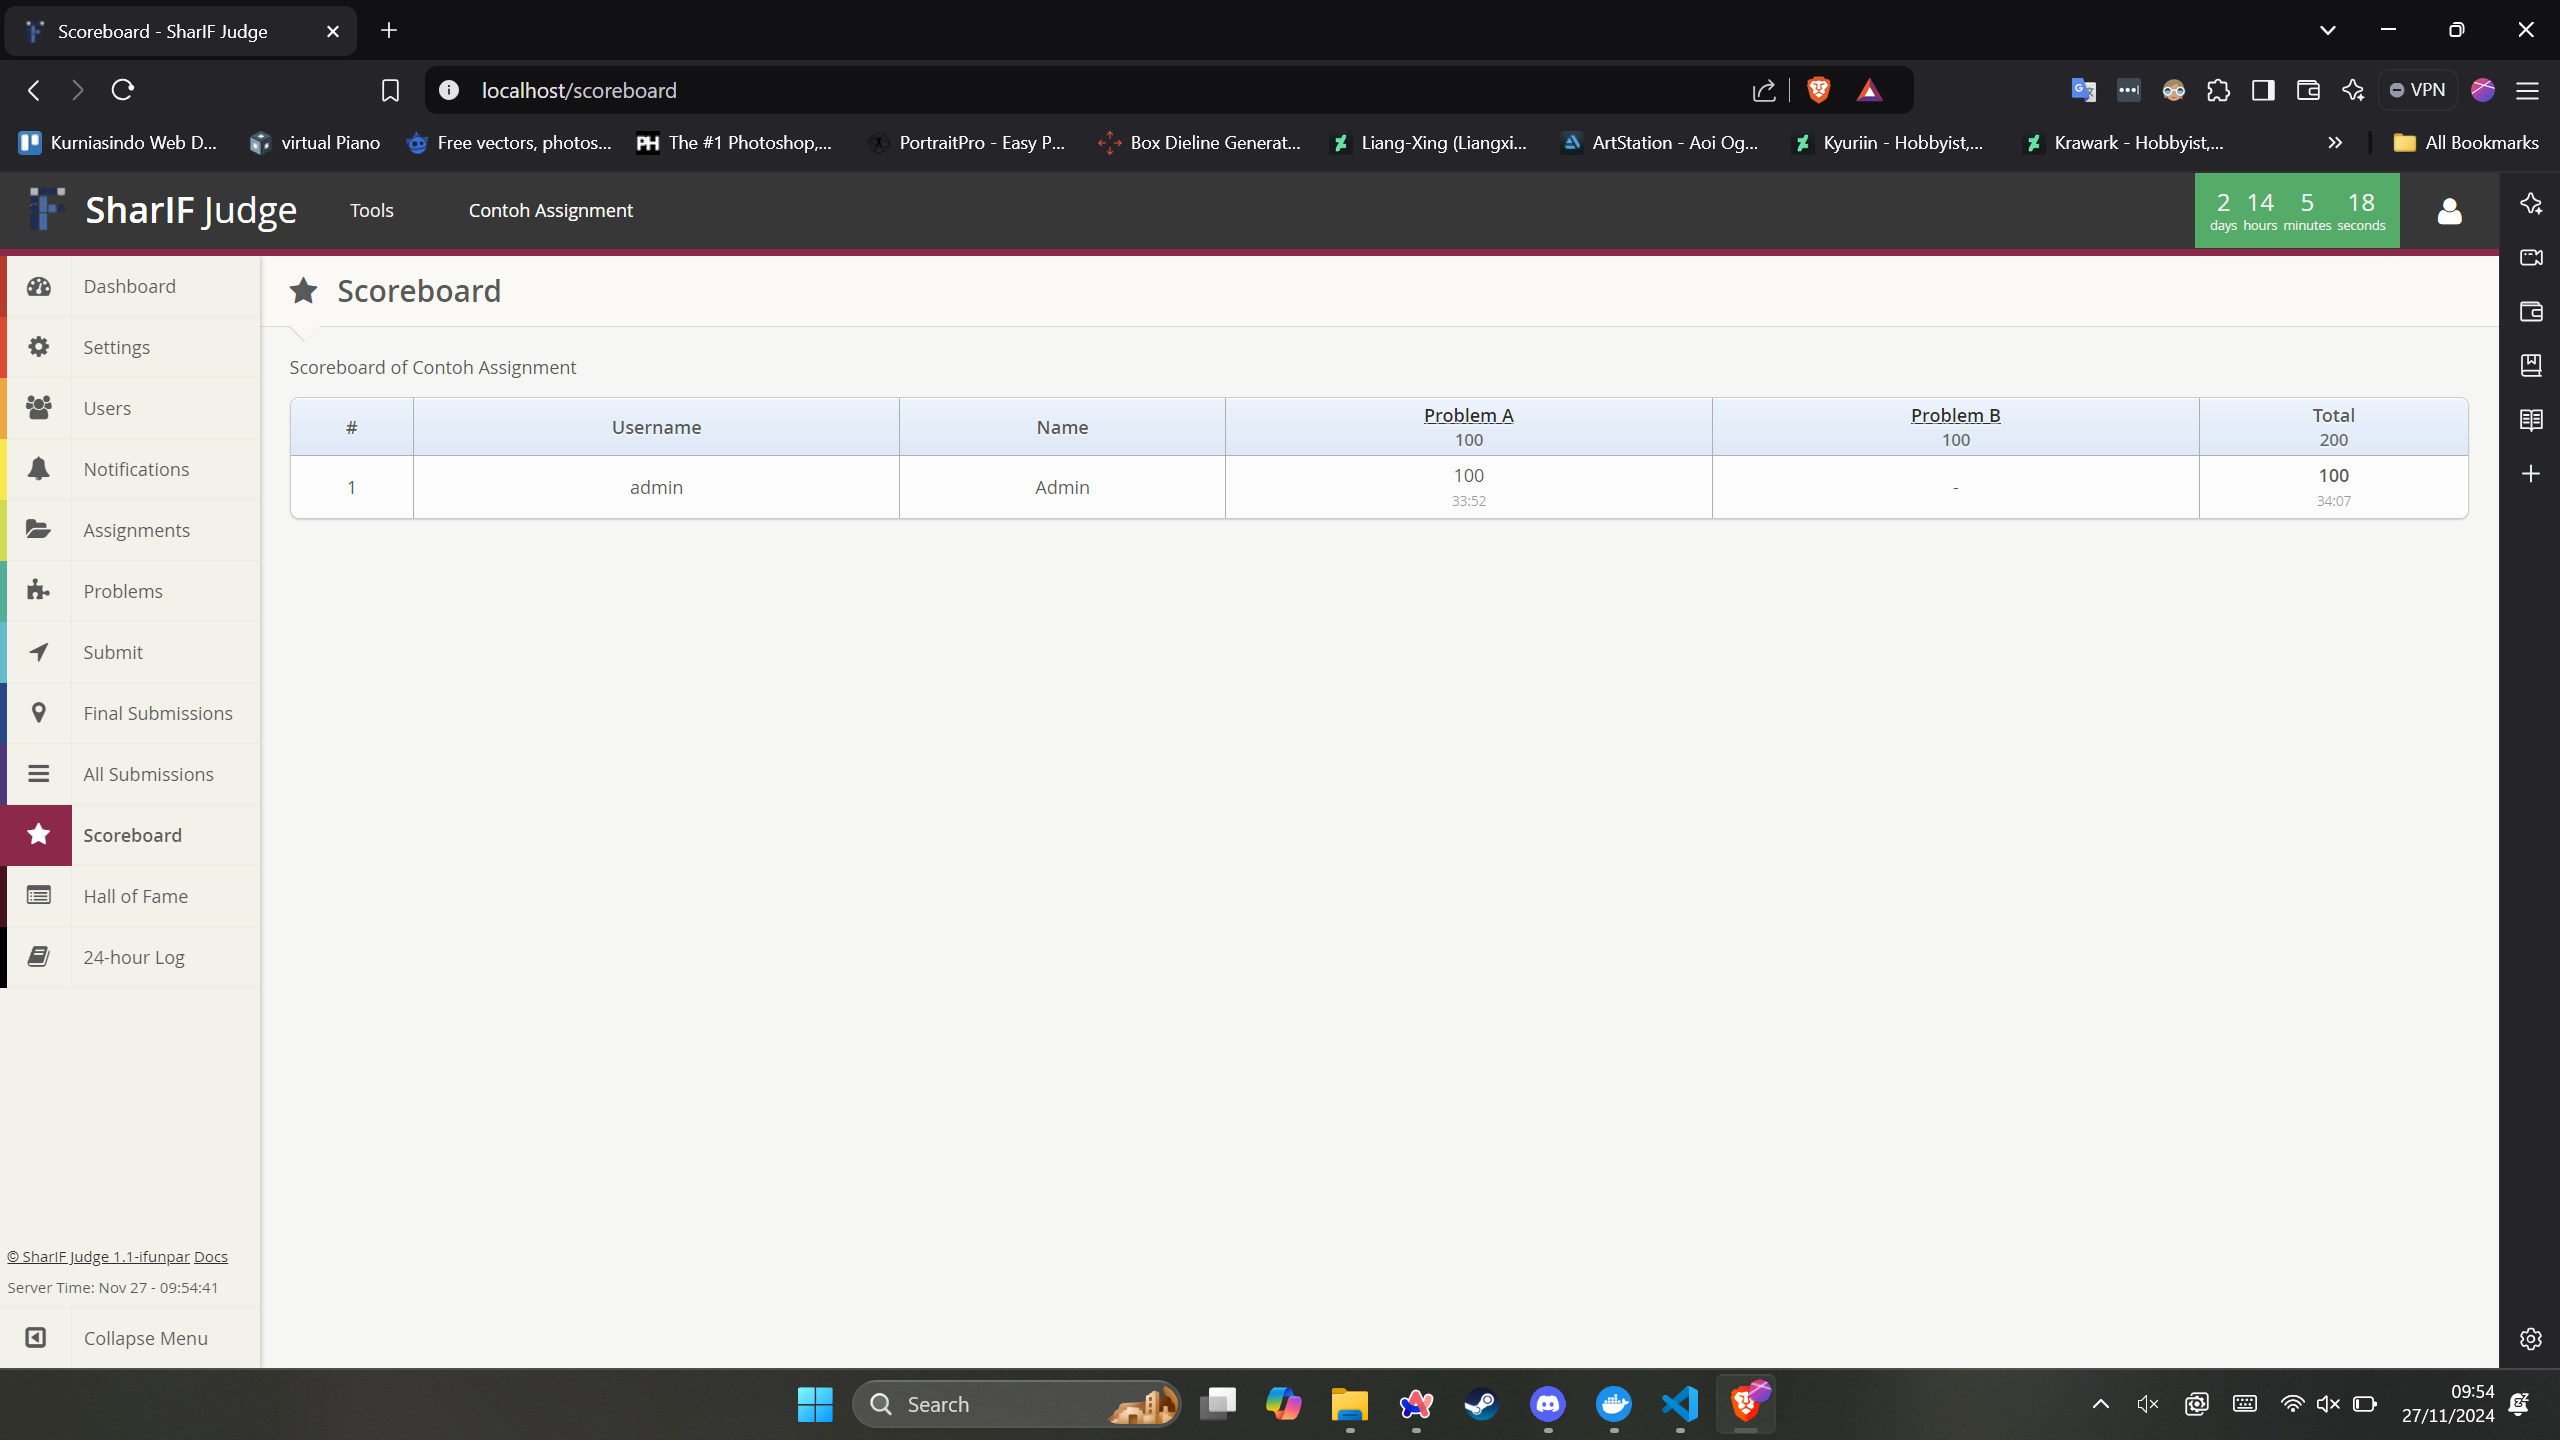
\includegraphics[width=0.875\textwidth]{views/scoreboard.png}
		      \caption{Halaman Scoreboard}
		      \label{fig:3:1:1:scoreboard}
	      \end{figure}

	\item \verb|Server_time.php| \\
	      \textit{Controller} \verb|Queueprocess.php| hanya memiliki satu fungsi yaitu \verb|index()| yang akan mencetak waktu pada \textit{server}, waktu akan digunakan untuk sinkronisasi waktu.

	\item \verb|Settings.php| \\
	      Berikut fungsi dengan penjelasannya pada \textit{controller} \verb|Settings.php|:

	      \begin{itemize}
		      \item \verb|update()| \\
		            Memperbaharui \textit{settings} dari masukkan pengguna.
		      \item \verb|index()| \\
		            Mendapatkan data dari \verb|Settings_model| dan menampilkan \textit{view} \verb|settings.twig|. Jika terdapat \textit{error setting} pada sistem, akan ditampilkan juga pada \textit{view} tersebut. Gambar \ref{fig:3:1:1:settings} menunjukkan hasil halaman Users.

		            \begin{figure}[H]
			            \centering
			            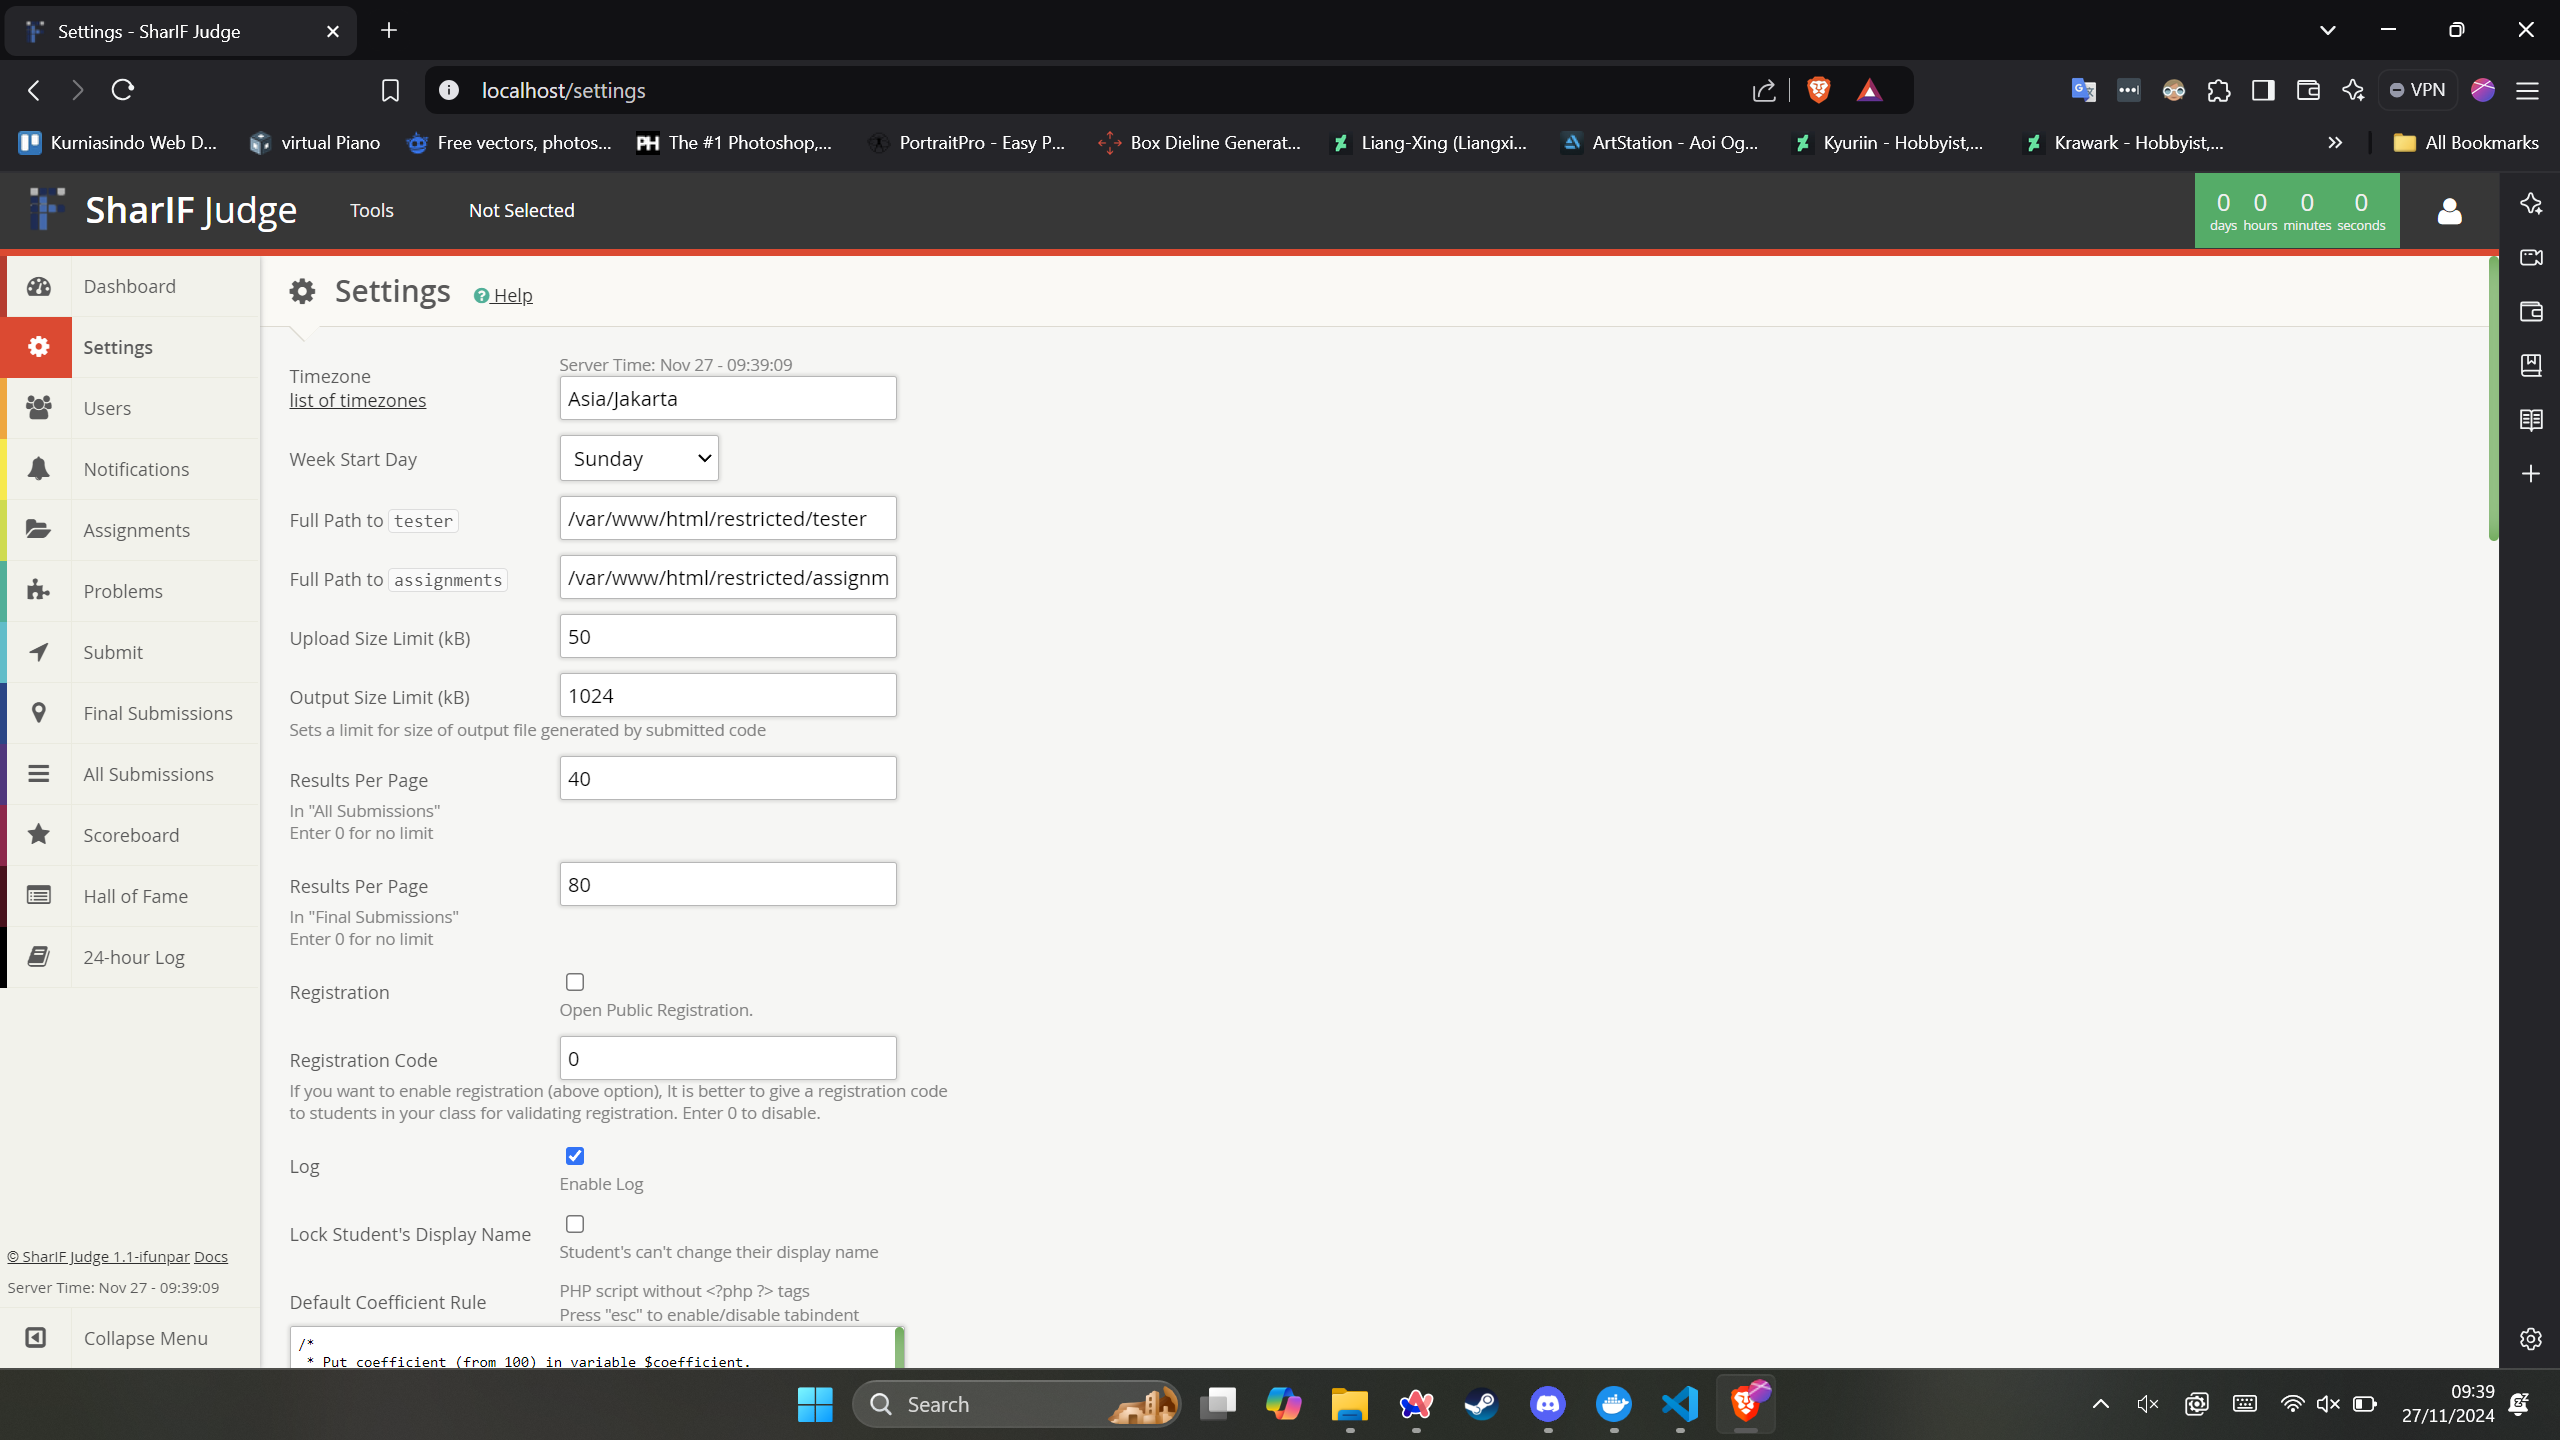
\includegraphics[width=0.875\textwidth]{views/settings.png}
			            \caption{Halaman Settings}
			            \label{fig:3:1:1:settings}
		            \end{figure}

	      \end{itemize}

	\item \verb|Submissions.php| \\
	      Berikut fungsi dengan penjelasannya pada \textit{controller} \verb|Submissions.php|:

	      \begin{itemize}
		      \item \verb|all()| \\
		            Fungsi ini akan mendapatkan data dari \verb|Submit_model| untuk mendapatkan seluruh \textit{submission} dan menampilkan halaman \verb|submission.twig| berisi semua \textit{submission}. Gambar \ref{fig:3:1:1:all} menunjukkan halaman All Submissions .

		            \begin{figure}
			            \centering
			            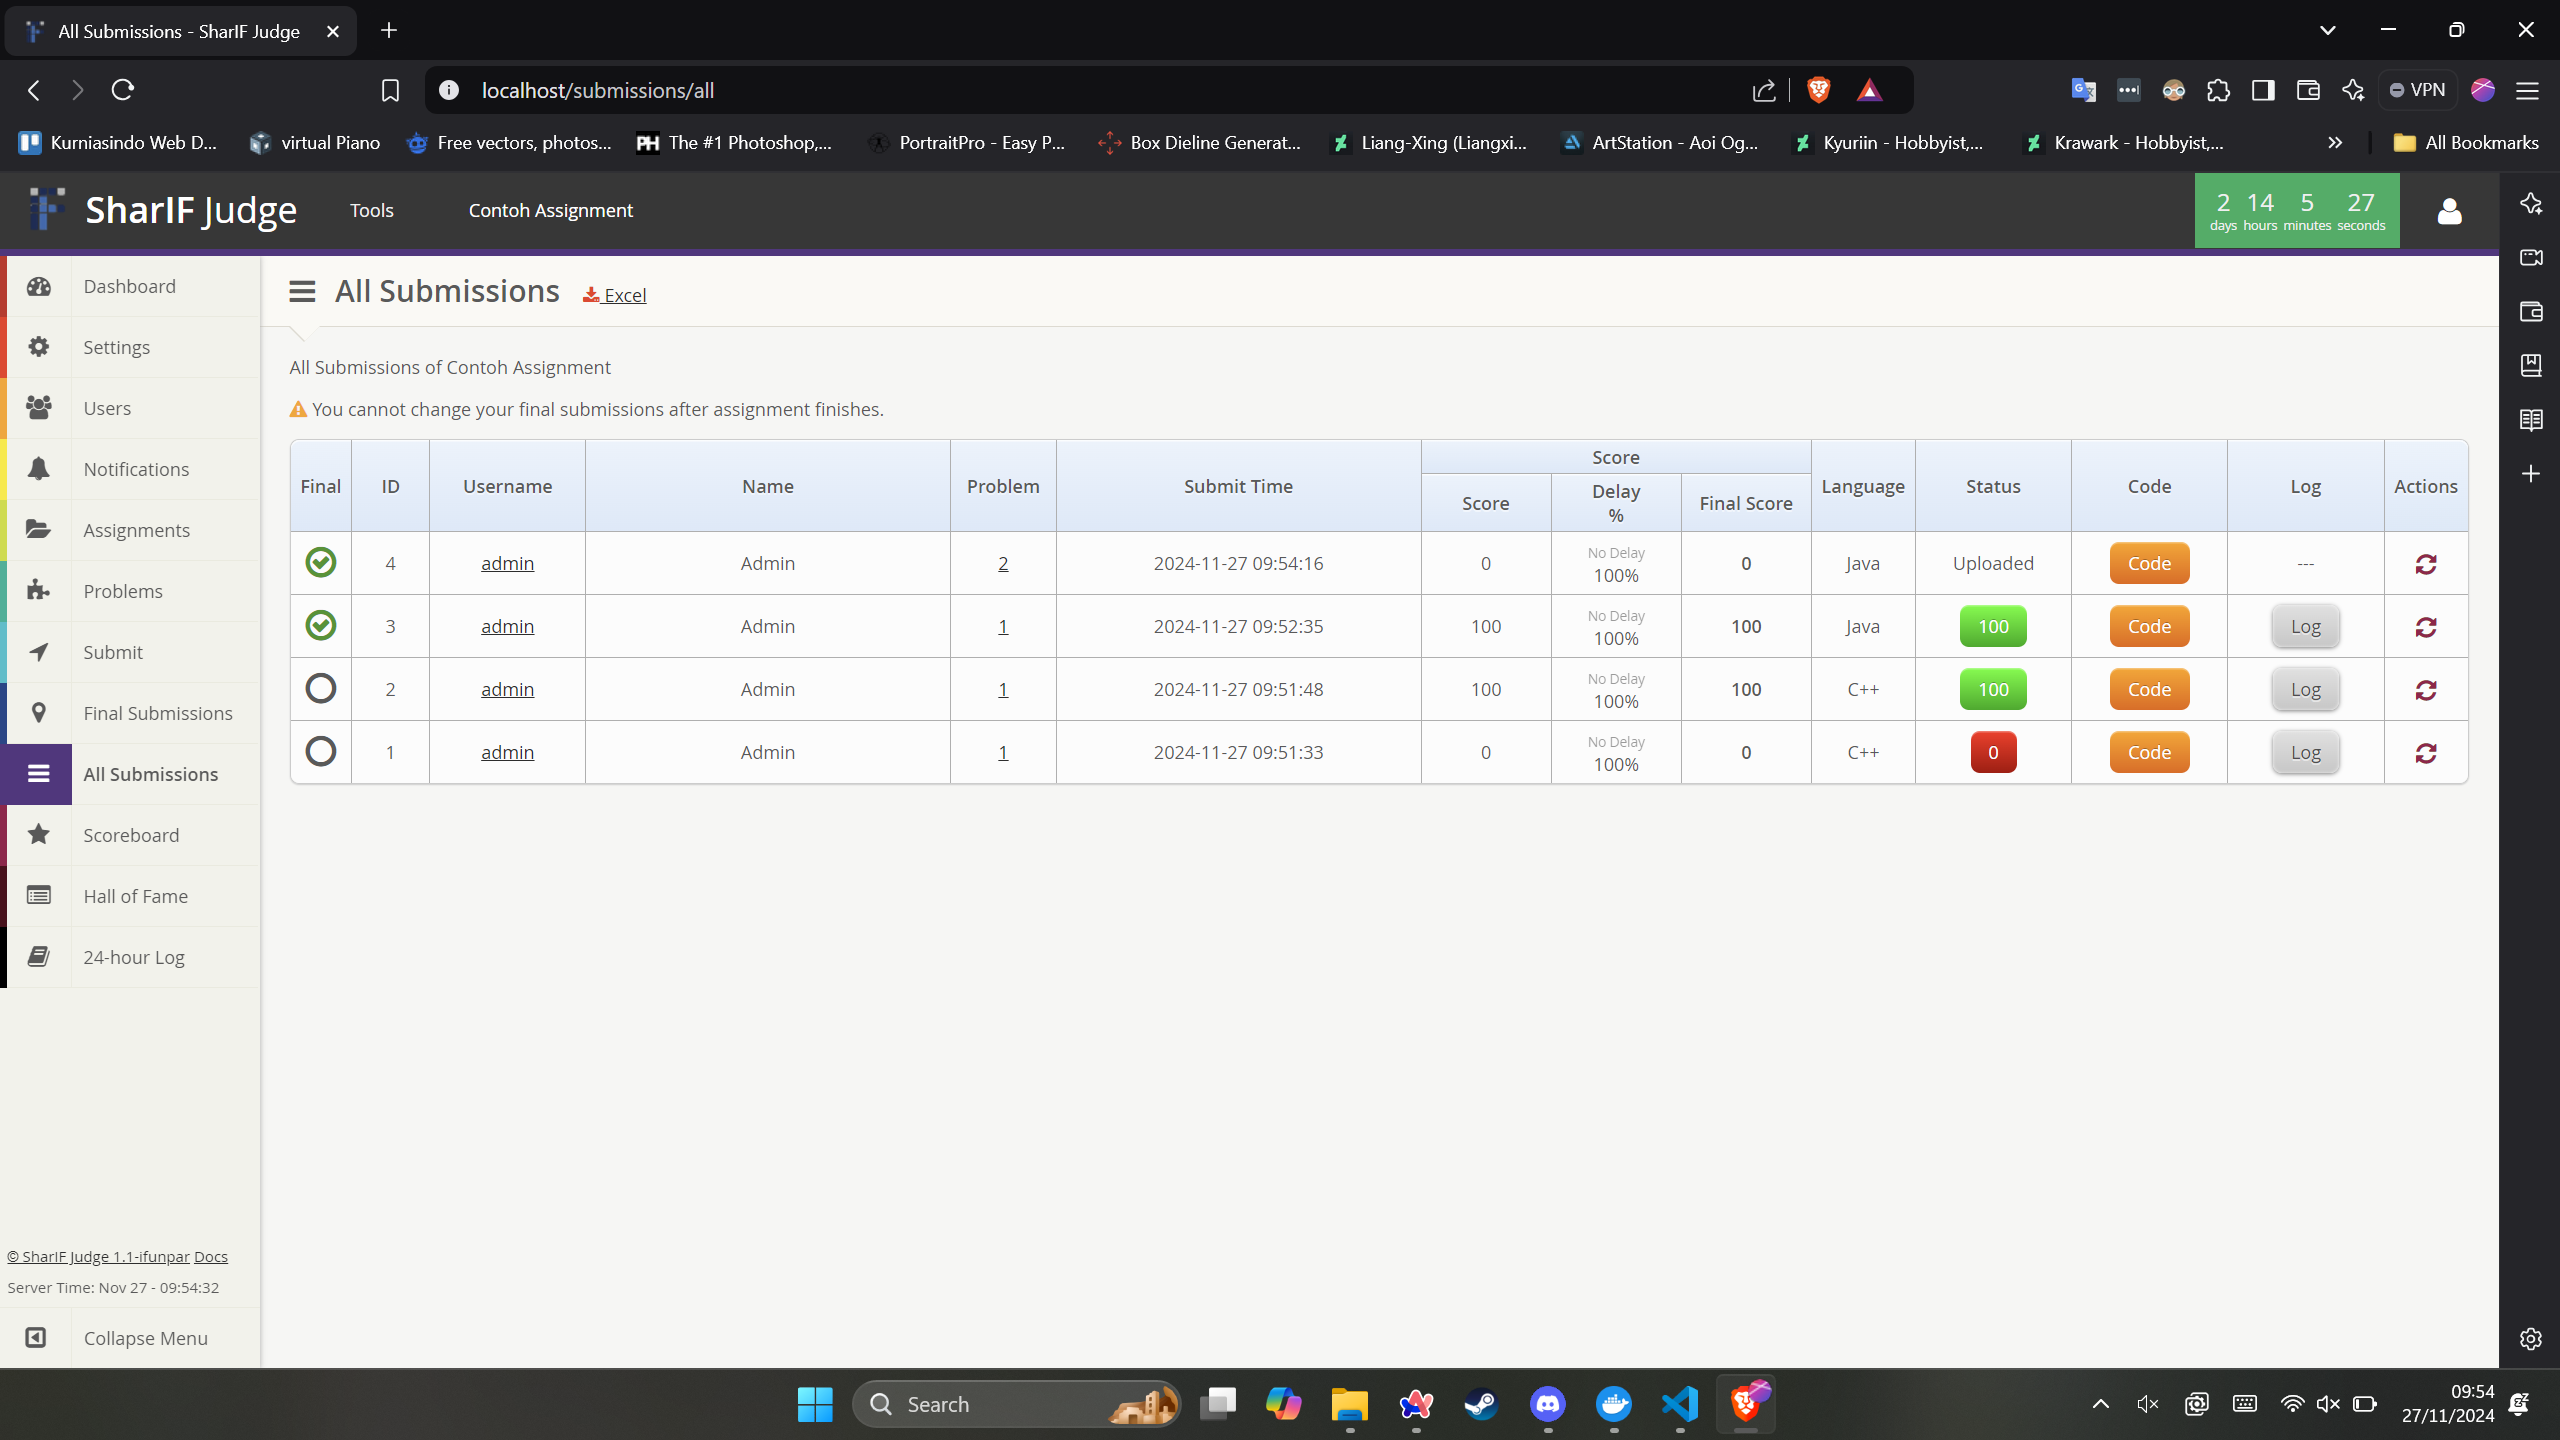
\includegraphics[width=0.825\textwidth]{views/all_submissions.png}
			            \caption{Halaman All Submissions}
			            \label{fig:3:1:1:all}
		            \end{figure}
		      \item \verb|the_final()| \\
		            Fungsi ini akan mendapatkan data dari \verb|Submit_model| untuk mendapatkan \textit{final submission} dan menampilkan halaman \verb|submission.twig| berisi \textit{final submission}. Gambar \ref{fig:3:1:1:final} menunjukkan halaman Final Submissions .
		            \begin{figure}[h]
			            \centering
			            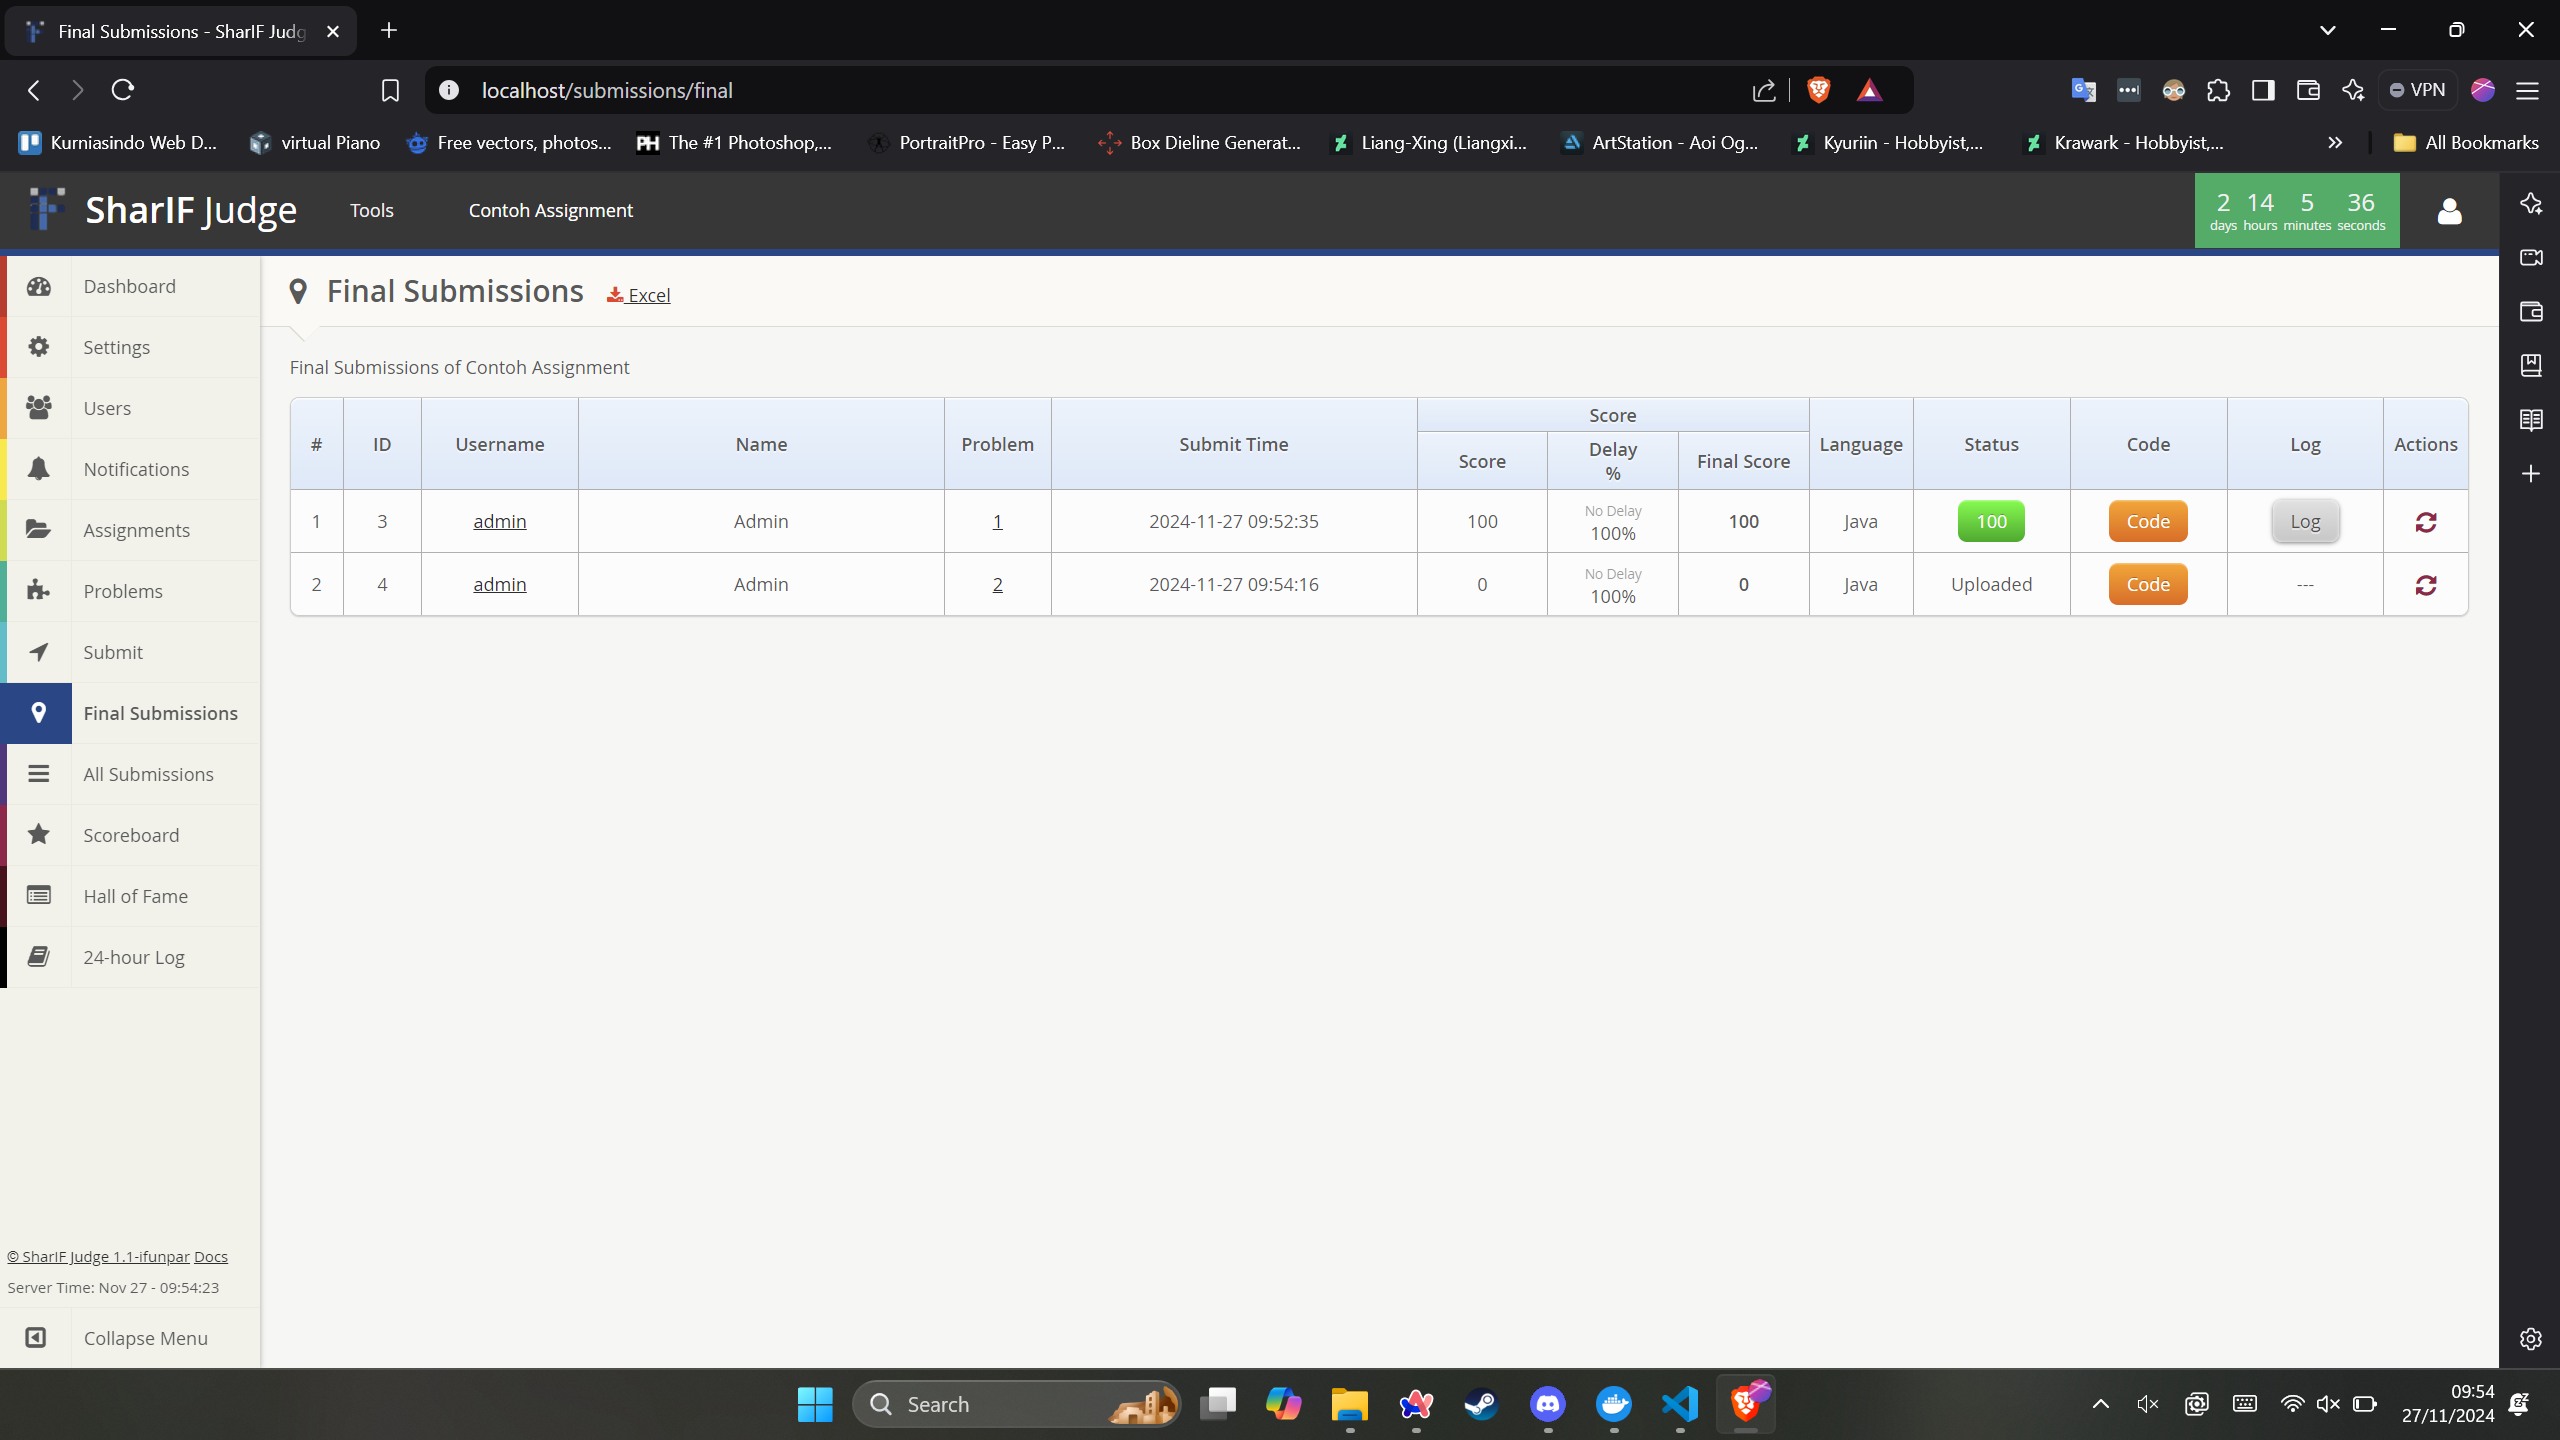
\includegraphics[width=0.825\textwidth]{views/final_submissions.png}
			            \caption{Halaman Final Submissions}
			            \label{fig:3:1:1:final}
		            \end{figure}
		      \item \verb|_download_excel($view)| \\
		            Fungsi ini menggunakan \textit{library} PHPExcel untuk membuat sebuah \textit{file excel} dari \textit{submissions} yang akan diunduh pengguna.
		      \item \verb|final_excel()| \\
		            Menggunakan fungsi \verb|_download_excel| untuk mendownload \textit{final submission}.
		      \item \verb|all_excel()| \\
		            Menggunakan fungsi \verb|_download_excel| untuk mendownload seluruh \textit{submission}.
		      \item \verb|select()| \\
		            Fungsi ini digunakan sebagai fungsi yang dipanggil oleh \textit{ajax request} untuk memilih \textit{submission} yang akan dikumpulkan atau menjadi \textit{final}.
		      \item \verb|_check_type($type)| \\
		            Melakukan validasi tipe \textit{submission} yang dikumpulkan.
		      \item \verb|view_code()| \\
		            Digunakan untuk melihat kode, melihat hasil kode, atau melihat \textit{log} sebuah \textit{submission}.
		      \item \verb|download_file()| \\
		            Mengunduh \textit{file} kode sebuah \textit{submission}.
	      \end{itemize}

	\item \verb|Submit.php| \\
	      Berikut fungsi dengan penjelasannya pada \textit{controller} \verb|Submit.php|:

	      \begin{itemize}
		      \item \verb|_language_to_type($language)| \\
		            Mengembalikan kode singkat dari \verb|$language| dipilih.
		      \item \verb|_language_to_ext($language)| \\
		            Mengembalikan extensi file dari \verb|$language| yang dipilih.
		      \item \verb|_match($type, $extension)| \\
		            Melakukan validasi untuk \verb|$type| dan \verb|$extension| agar sesuai.
		      \item \verb|_check_language($str)| \\
		            Melakukan validasi sudah dipilihannya bahasa.
		      \item \verb|_upload()| \\
		            Menyimpan jawaban pengguna yang dikirim dan menambahkannya ke dalam \textit{queue} untuk dinilai jika bukan \textit{upload only problem}.
		      \item \verb|load($problem_id)| \\
		            Mendapatkan isi file dan menyimpan isi file ke editor kode.
		      \item \verb|save($type)| \\
		            Fungsi ini digunakan untuk menyimpan isi editor kode ke dalam \textit{server} dan menjalankan atau mengumpulkan jika diinginkan.
		      \item \verb|_submit($data, $problem_id, $language, $user_dir)| \\
		            Menambahkan kode ke dalam \textit{submission} untuk dinilai.
		      \item \verb|_execute($data, $problem_id, $language, $user_dir)| \\
		            Menambahkan kode ke dalam \textit{queue} untuk dijalankan saja.
		      \item \verb|get_output($problem_id)| \\
		            Mendapatkan keluaran dari kode yang telah dijalankan sebagai hasil eksekusi.
		      \item \verb|index()| \\
		            Fungsi ini akan mendapatkan data dari \textit{model} \verb|Assignments_model| untuk mendapatkan \textit{problem} dan data lainnya. Semua data tersebut akan dimasukkan dalam \textit{view} \verb|submit.twig|. Gambar \ref{fig:3:1:1:submit} menunjukkan hasil halaman Submit. Halaman ini terdapat editor kode yang sudah diimplementasikan~\cite{nicholas:sharif}.

		            \begin{figure}
			            \centering
			            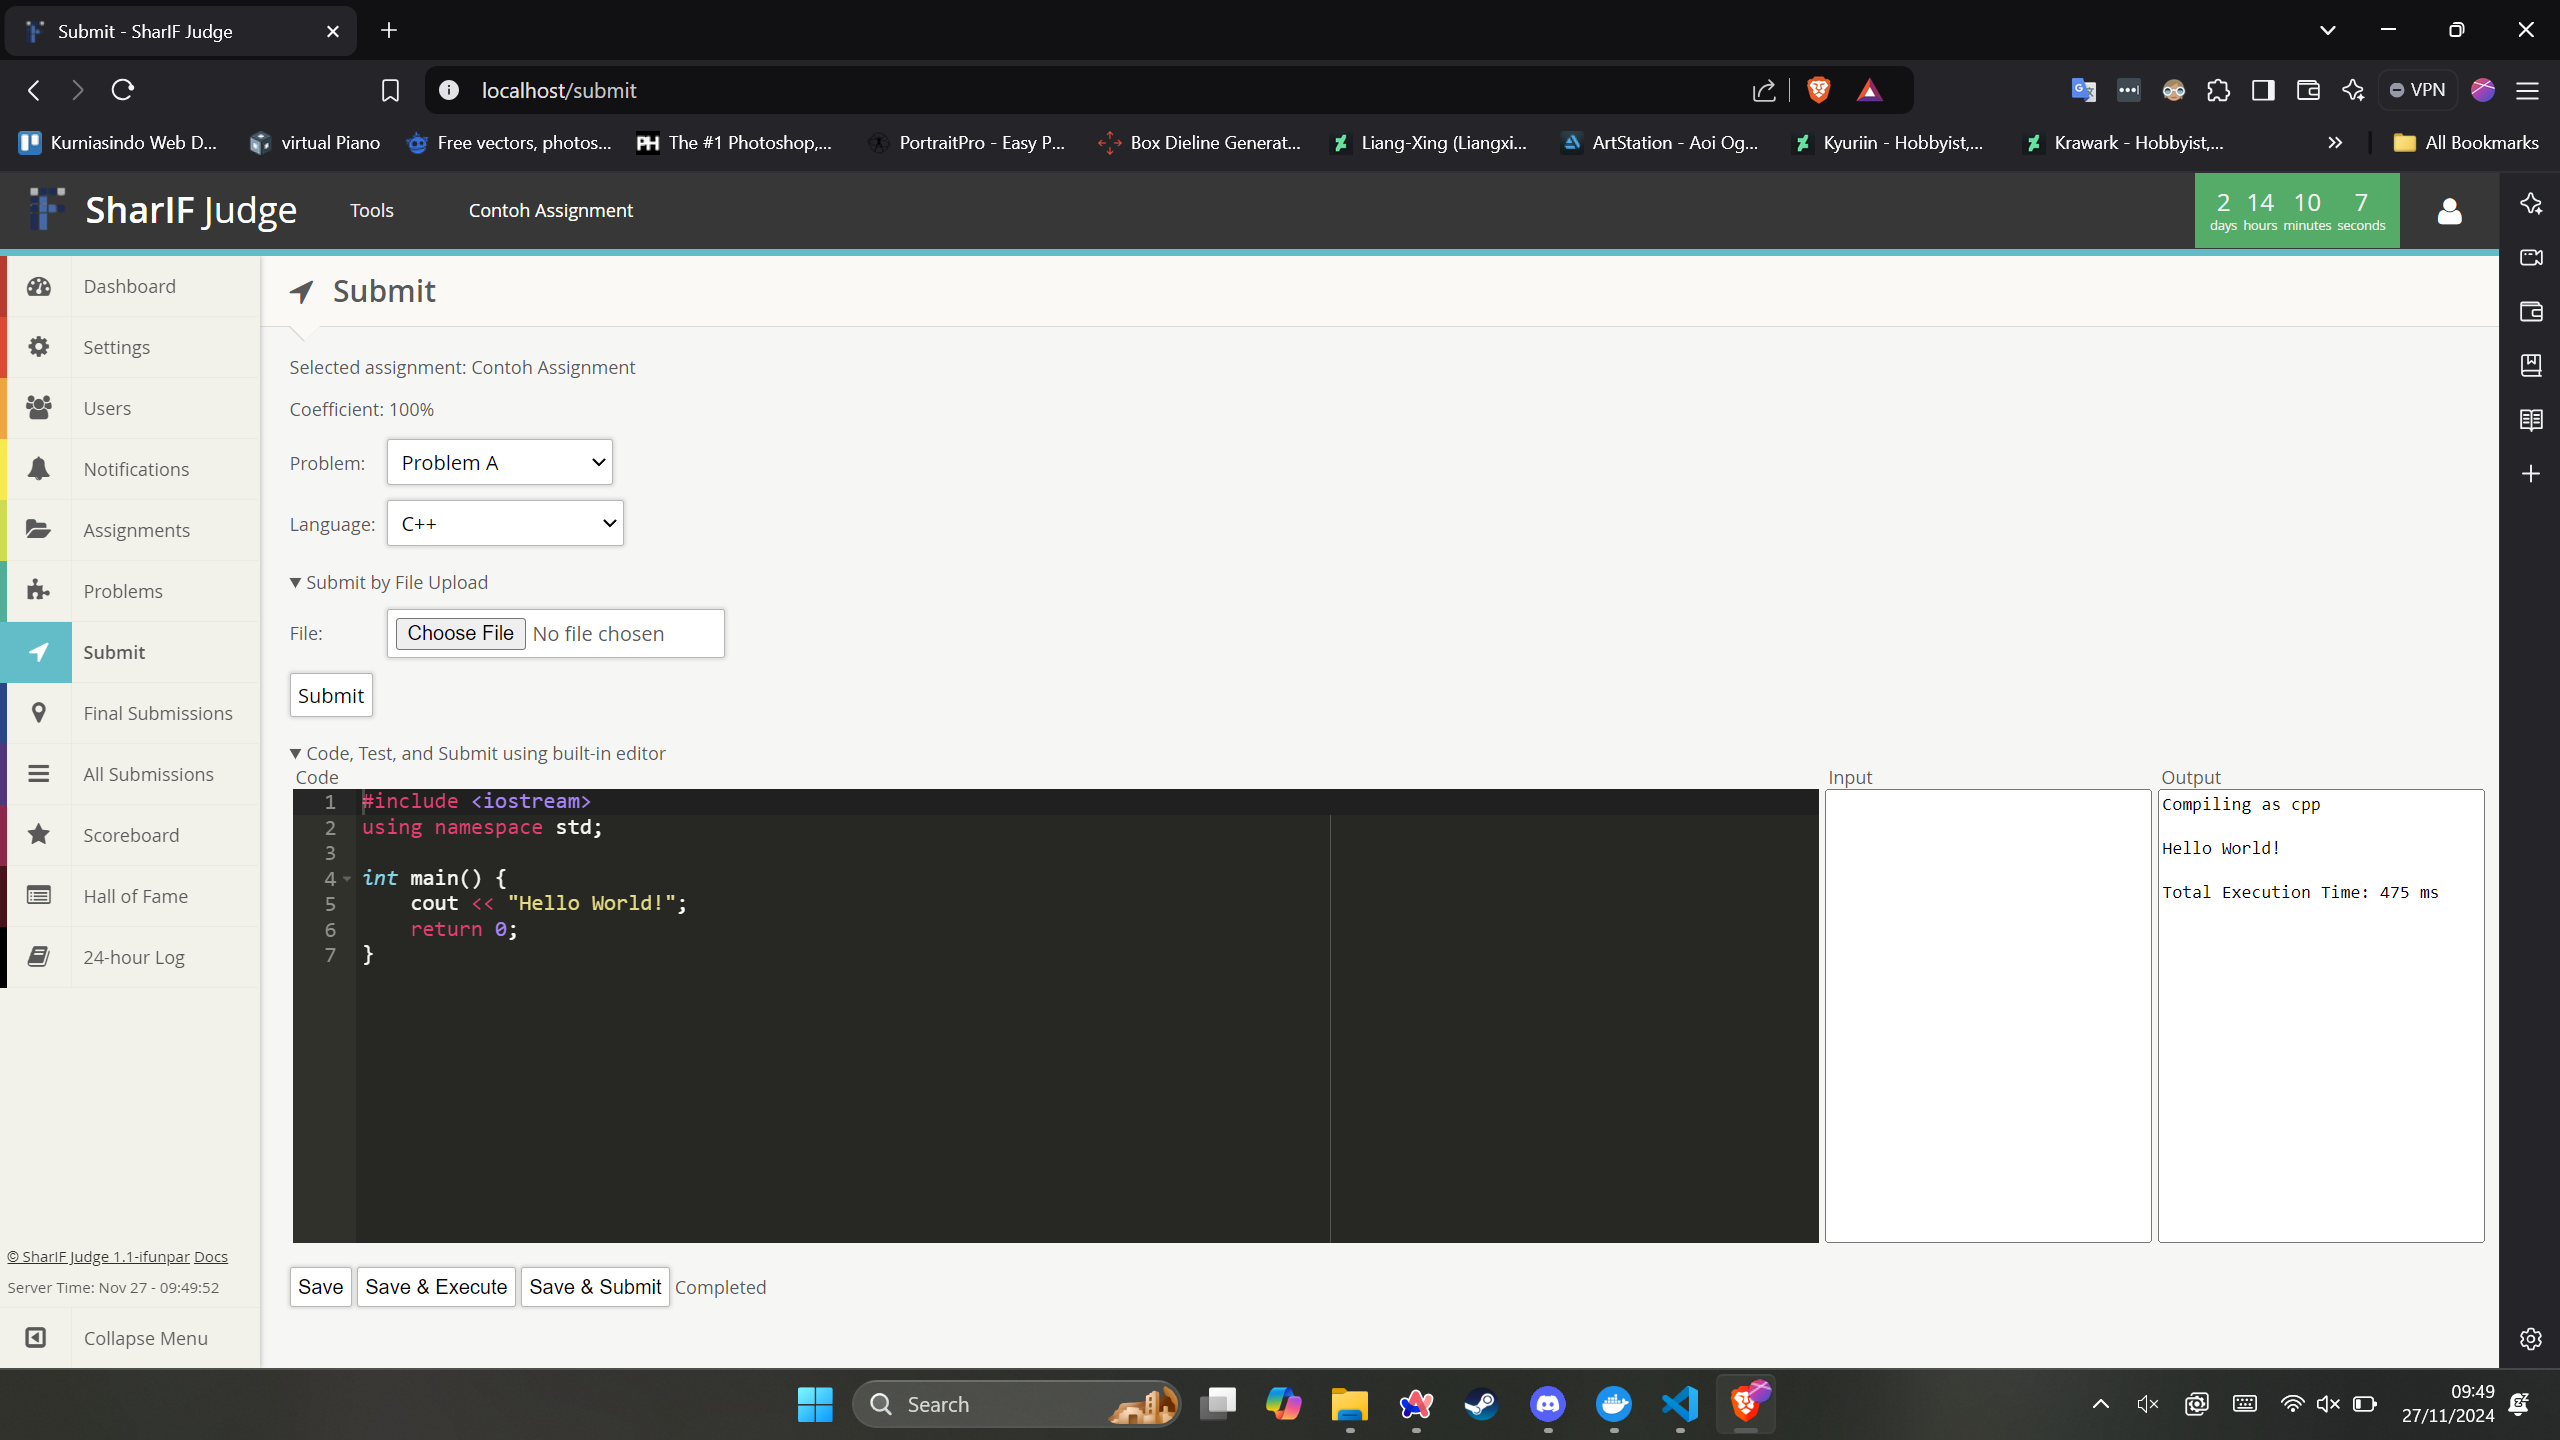
\includegraphics[width=0.85\textwidth]{views/submit.png}
			            \caption{Halaman Submit}
			            \label{fig:3:1:1:submit}
		            \end{figure}

	      \end{itemize}

	\item \verb|User.php| \\
	      Berikut fungsi dengan penjelasannya pada \textit{controller} \verb|User.php|:

	      \begin{itemize}
		      \item \verb|add()| \\
		            Menambahkan pengguna baru ke dalam \textit{sistem}.
		      \item \verb|delete()| \\
		            Menghapus sebuah pengguna.
		      \item \verb|delete_submissions()| \\
		            Menghapus seluruh \textit{submissions} dari sebuah pengguna.
		      \item \verb|list_excel()| \\
		            Menggunakan \textit{library} PHPExcel untuk membuat sebuah file excel dari seluruh daftar pengguna yang akan diunduh pengguna.
		      \item \verb|index()| \\
		            Fungsi ini akan mendapatkan data dari \verb|User_model| dan menunjukkan \textit{view} \verb|users.twig| menggunakan data tersebut. Gambar \ref{fig:3:1:1:users} menunjukkan hasil halaman Users. Pada halaman ini terdapat daftar seluruh pengguna yang terdaftar pada SharIF Judge. Pengguna dapat membuat, memperbaharui, dan menghapus pengguna.

		            \begin{figure}[H]
			            \centering
			            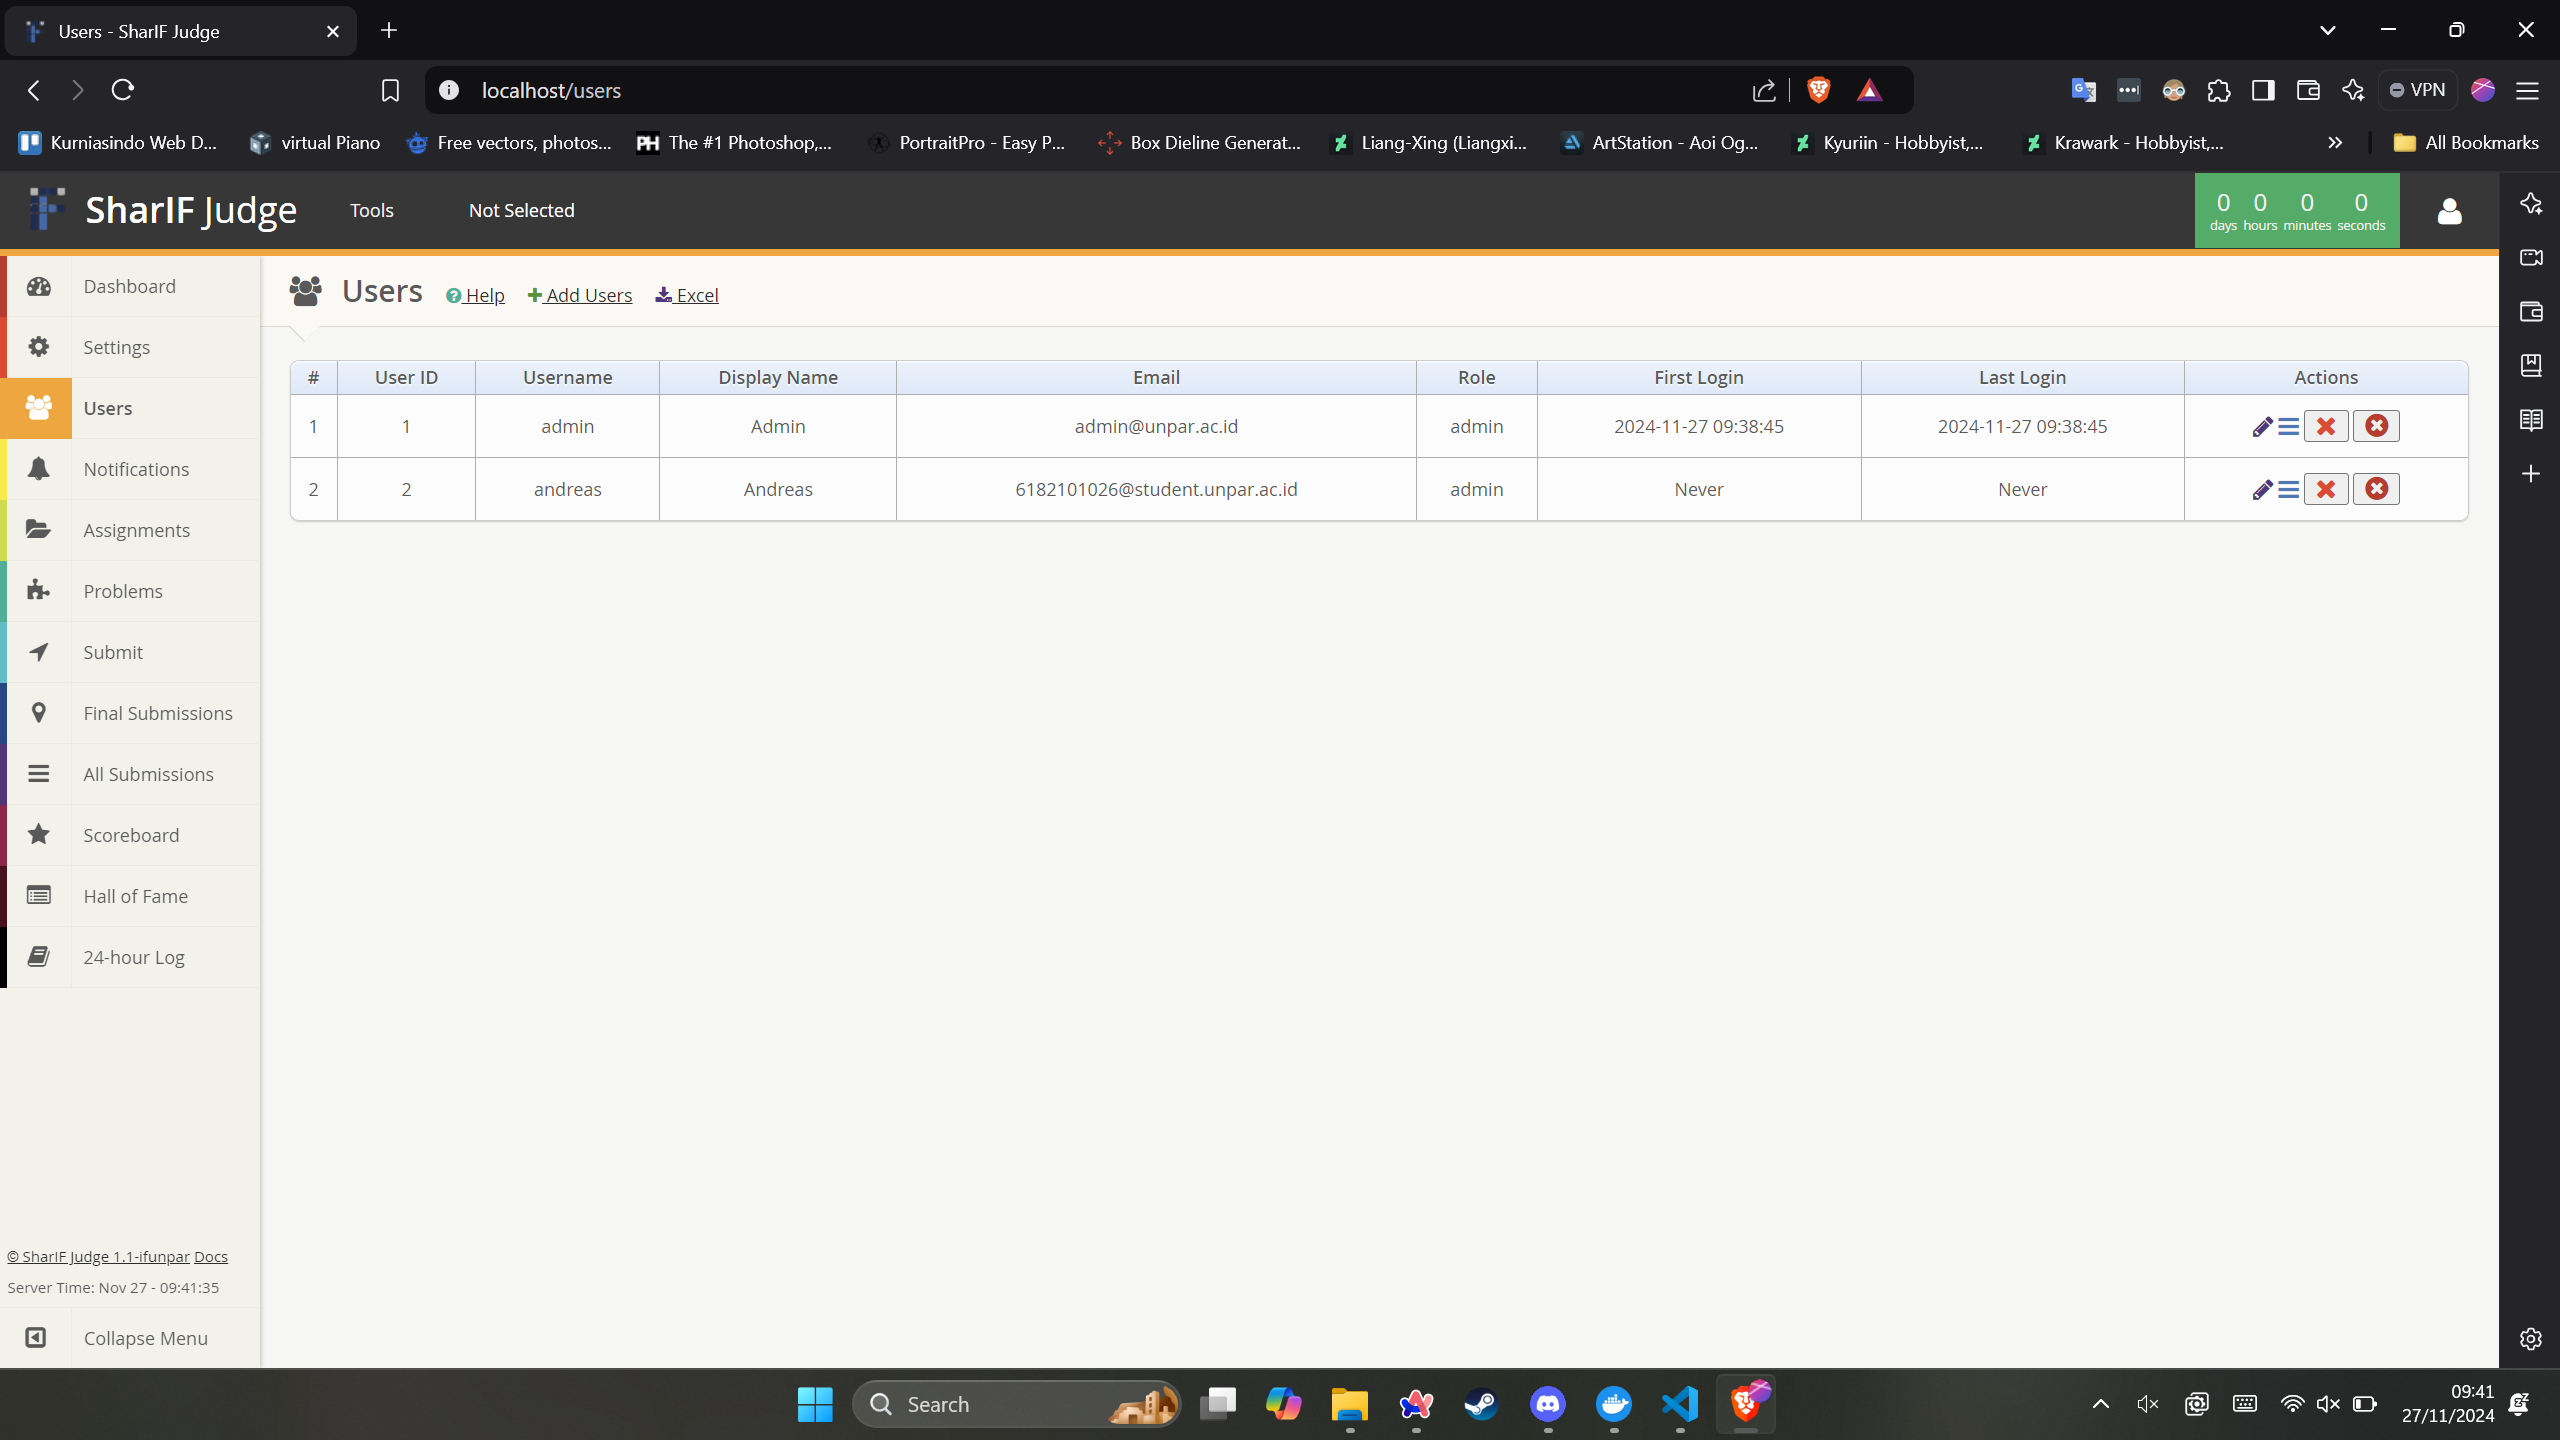
\includegraphics[width=0.85\textwidth]{views/users.png}
			            \caption{Halaman Users}
			            \label{fig:3:1:1:users}
		            \end{figure}


	      \end{itemize}

\end{itemize}

\subsection{Assets}
Pada SharIF Judge terdapat direktori bernama \textit{Assets} yang menjadi tempat untuk menyimpan seluruh kebutuhan dari sisi pengguna seperti gambar logo dan \textit{library JavaScript}. Berikut merupakan isi dari direktori \textit{assets} beserta dengan kegunaannya dalam aplikasi SharIF Judge:

\begin{itemize}
	\item Direktori \verb|ace| \\
	      Direktori ini berisi hasil \textit{build library} Ace, menghasilkan file \textit{JavaScript} yang berfungsi untuk menambahkan editor kode pada aplikasi.
	\item Direktori \verb|font| \\
	      Direktori ini berisi font khusus dan juga memiliki \textit{library JavaScript} bernama font-awesome yang digunakan untuk menyimpan icon berformat svg dalam tampilan SharIF Judge.
	\item Direktori \verb|fullcalendar| \\
	      Direktori ini berisi hasil \textit{build library} FullCalendar, menghasilkan file \textit{JavaScript} dan \textit{css} yang berfungsi untuk memasukkan kalendar dalam tampilan SharIF Judge.
	\item Direktori \verb|gridster| \\
	      Direktori ini berisi hasil \textit{build plugin} Gridster yang menggunakan \textit{library} jQuery, menghasilkan file \textit{JavaScript} dan \textit{css} yang berfungsi untuk memasukkan \textit{layout} grid yang dapat diubah dengan menggunakan sifat mouse \textit{drag and drop}.
	\item Direktori \verb|images| \\
	      Direktori ini berisi gambar kustom yang digunakan oleh SharIF Judge seperti logo universitas dan banner universitas dalam situs web.
	\item Direktori \verb|js| \\
	      Direktori ini berisi hasil \textit{build library} jQuery, taboverride, moment, \textit{plugins} jQuery untuk membantu \textit{JavaScript} khusus yang dipakai dalam SharIF Judge. Direktori ini juga memiliki file \textit{JavaScript} khusus yang dipakai dalam halaman SharIF Judge yaitu sebagai berikut:
	      \begin{itemize}
		      \item \verb|shj_functions.js| \\
		            File \textit{JavaScript} \verb|shj_functions| digunakan untuk seluruh sistem umum dalam SharIF Judge seperti waktu server, sidebar \textit{toggle}, loading dan berbagai macam fungsi yang digunakan dalam SharIF Judge.
		      \item \verb|shj_submissions.js| \\
		            File \textit{JavaScript} \verb|shj_submissions| digunakan untuk menangani berbagai fitur untuk halaman all submissions dan final submissions seperti menampilkan kode program dan memeriksa ulang hasil kode dalam judge.
		      \item \verb|shj_submit.js| \\
		            File \textit{JavaScript} \verb|shj_submit| digunakan untuk menangani berbagai fitur untuk halaman submit terutama fungsi aksi pada IDE yaitu aksi \textit{save}, \textit{execute}, \textit{submit}, dan memuat kode lama ke dalam editor kode.
	      \end{itemize}
	\item Direktori \verb|nano_scroller| \\
	      Direktori ini berisi hasil \textit{build plugin} nanoScrollerJS untuk \textit{library} jQuery, menghasilkan file \textit{JavaScript} dan \textit{css} yang berfungsi untuk membangun \textit{scrollbar} pada SharIF Judge.
	\item Direktori \verb|noty| \\
	      Direktori ini berisi \textit{plugin} noty untuk \textit{library} jQuery, menghasilkan file \textit{JavaScript} dan \textit{css} yang berfungsi untuk menampilkan pesan atau notifikasi kepada pengguna pada SharIF Judge.
	\item Direktori \verb|pdfjs| \\
	      Direktori ini berisi hasil \textit{build library} pdfjs, menghasilkan file \textit{JavaScript} yang berfungsi untuk menampilkan file pdf pada SharIF Judge.
	\item Direktori \verb|reveal| \\
	      Direktori ini berisi hasil \textit{build plugin} Reveal yang sudah dimodifikasi untuk \textit{library} jQuery, menghasilkan file \textit{JavaScript} dan \textit{css} yang berfungsi untuk menampilkan \textit{modal} konfirmasi.
	\item Direktori \verb|snippet| \\
	      Direktori ini berisi hasil \textit{build plugin} Snippet yang sudah dimodifikasi untuk \textit{library} jQuery, berfungsi untuk sebagai \textit{Syntax Highlighter} untuk teks kode dalam halaman Hall of Fame, Problems, dan Submissions.
	\item Direktori \verb|styles| \\
	      Direktori ini berisi seluruh \textit{Cascading Style Sheets} atau css \textit{file} khusus yang digunakan untuk memperindah halaman web dalam SharIF Judge.
	\item Direktori \verb|tinymce| \\
	      Direktori ini berisi hasil \textit{build library} tinymce yang berfungsi  untuk memasukkan editor teks pada halaman \textit{Submission}, \textit{Final Submission} dalam SharIF Judge.
\end{itemize}

\subsection{Penyimpanan Kode Submission}
\label{sub:3:1:penyimpanankode}
Pada SharIF Judge, Kode akan disimpan pada lokasi \verb|Assignment| yang dapat diubah pada halaman \verb|Settings|. Berikut merupakan format penyimpanan sebuah kode:

\begin{center}
	\verb|assignment_<a_id>/p<p_id>/<nama user>/<nama file>-<s_id>.<file ext>|
\end{center}

Penjelasan untuk format di atas adalah sebagai berikut:

\begin{itemize}
	\item \verb|<a_id>| \\
	      \verb|id| pada \textit{assignment}.
	\item \verb|<p_id>| \\
	      \verb|id| pada \textit{problem}.
	\item \verb|<nama user>| \\
	      Nama dari pengguna yang mengumpulkan kode/file.
	\item \verb|<nama file>| \\
	      Nama file yang dikumpulkan, \verb|editor| jika mengumpulkan menggunakan editor kode.
	\item \verb|<s_id>| \\
	      \verb|id| pada \textit{submission}.
	\item \verb|<file ext>| \\
	      Extensi file kode yang dikumpulkan.
\end{itemize}

Sebagai contoh, pengguna bernama \verb|kenzhi| mengumpulkan kode dengan nama file \verb|probA.java| ke dalam \textit{problem} pertama dari \textit{assignment} dengan id 5. \verb|kenzhi| sudah melakukan pengumpulan pada \textit{problem} yang sama sebanyak 5 kali dan \textit{submission} kali ini akan menjadi nomor 6, sehingga \verb|submission id| adalah 6. Maka kode pengguna akan disimpan pada alamat:

\begin{center}
	\verb|assignment_5/p1/kenzhi/probA-6.java|
\end{center}

\subsection{Antrean Penilaian Kode}
\label{sub:3:1:antreanpenilaiankode}

Pada SharIF Judge, Kode yang dikumpulkan akan dijalankan satu per satu pada antrean menggunakan \verb|bash|. Berikut merupakan cara SharIF Judge menilai kode dari awal pengumpulan pada sistem:

\begin{enumerate}
	\item \textit{Controller} \verb|Submit| akan menyimpan kode ke dalam \textit{file} pada direktori sesuai pada \ref{sub:3:1:penyimpanankode}.
	\item \textit{Controller} \verb|Submit| akan memasukkan data \textit{submission} ke dalam \textit{model} \verb|Queue_model|.
	\item \textit{Model} \verb|Queue_model| akan menyimpan data \textit{submission} pada \textit{database} \verb|submission| dan menambahkan data \verb|queue|.
	\item Selanjutnya \textit{Controller} \verb|Submit| akan memanggil fungsi \verb|process_the_queue()| yang akan menjalankan fungsi \verb|run()| pada \textit{controller} \verb|Queueprocess|.
	\item \verb|Queueprocess| akan menjalankan \verb|tester.sh| pada direktori \verb|tester| dengan data dari \verb|queue|.
	\item Selanjutnya \verb|tester.sh| akan menilai kode program sesuai dengan \textit{input} dan \textit{output} yang diinginkan. Lalu penilaian akan dibaca dan disimpan oleh \textit{controller} \verb|Queueprocess|.
	\item Terakhir \verb|Queueprocess| akan menyimpan hasil penilaian pada \textit{database} \verb|submission| dan menghapus data \verb|queue| menggunakan \verb|Queue_model|.
\end{enumerate}

\subsection{Editor Kode}

Integrated Development Environment (IDE) pada SharIF Judge dirancang dengan antarmuka yang terdiri atas empat komponen utama, yaitu sebagai berikut:

\begin{itemize}
	\item Editor Kode \\
	      Editor kode ditandai dengan warna merah dalam Gambar~\ref{fig:3:1:editorkode} merupakan area utama tempat pengguna menulis dan mengedit kode program. Editor ini dilengkapi dengan fitur syntax highlighting dan auto-indent untuk mendukung produktivitas pengguna.
	\item Editor Input \\
	      Editor Input ditandai dengan warna biru dalam Gambar~\ref{fig:3:1:editorkode} berfungsi sebagai tempat pengguna memasukkan data uji yang akan digunakan saat menjalankan program melalui aksi Execute. Input yang dimasukkan akan diproses sebagai \textit{standard input} atau \textit{stdin} saat kode dijalankan.
	\item Editor Output \\
	      Editor Output ditandai dengan warna hijau dalam Gambar~\ref{fig:3:1:editorkode} menampilkan hasil eksekusi kode program, termasuk keluaran, pesan kesalahan jika ada, dan waktu komputasi. Konten pada bagian ini dihasilkan secara otomatis setiap aksi Execute dilakukan.
	\item Tombol Aksi \\
	      Tombol Aksi ditandai dengan warna kuning dalam Gambar~\ref{fig:3:1:editorkode} menyediakan tiga tombol aksi interaksi yaitu sebagai berikut:
	\item PDF Viewer \\
	      PDF Viewer ditandai dengan warna kuning dalam Gambar~\ref{fig:3:1:editorkode} merupakan sebuah komponen dalam IDE yang digunakan untuk menampilkan soal atau instruksi tugas kepada mahasiswa.

	      \begin{itemize}
		      \item \textbf{\textit{Save}}: Menyimpan sementara kode program tanpa menjalankan atau mengumpulkannya.
		      \item \textbf{\textit{Save \& Execute}}: Menyimpan kode sekaligus menjalankannya dengan input yang tersedia di Editor Input. Hasilnya ditampilkan di Editor Output.
		      \item \textbf{\textit{Save \& Submit}}: Menyimpan dan mengumpulkan kode sebagai submission untuk dinilai oleh SharIF Judge.
	      \end{itemize}
\end{itemize}

\begin{figure}[H]
	\centering
	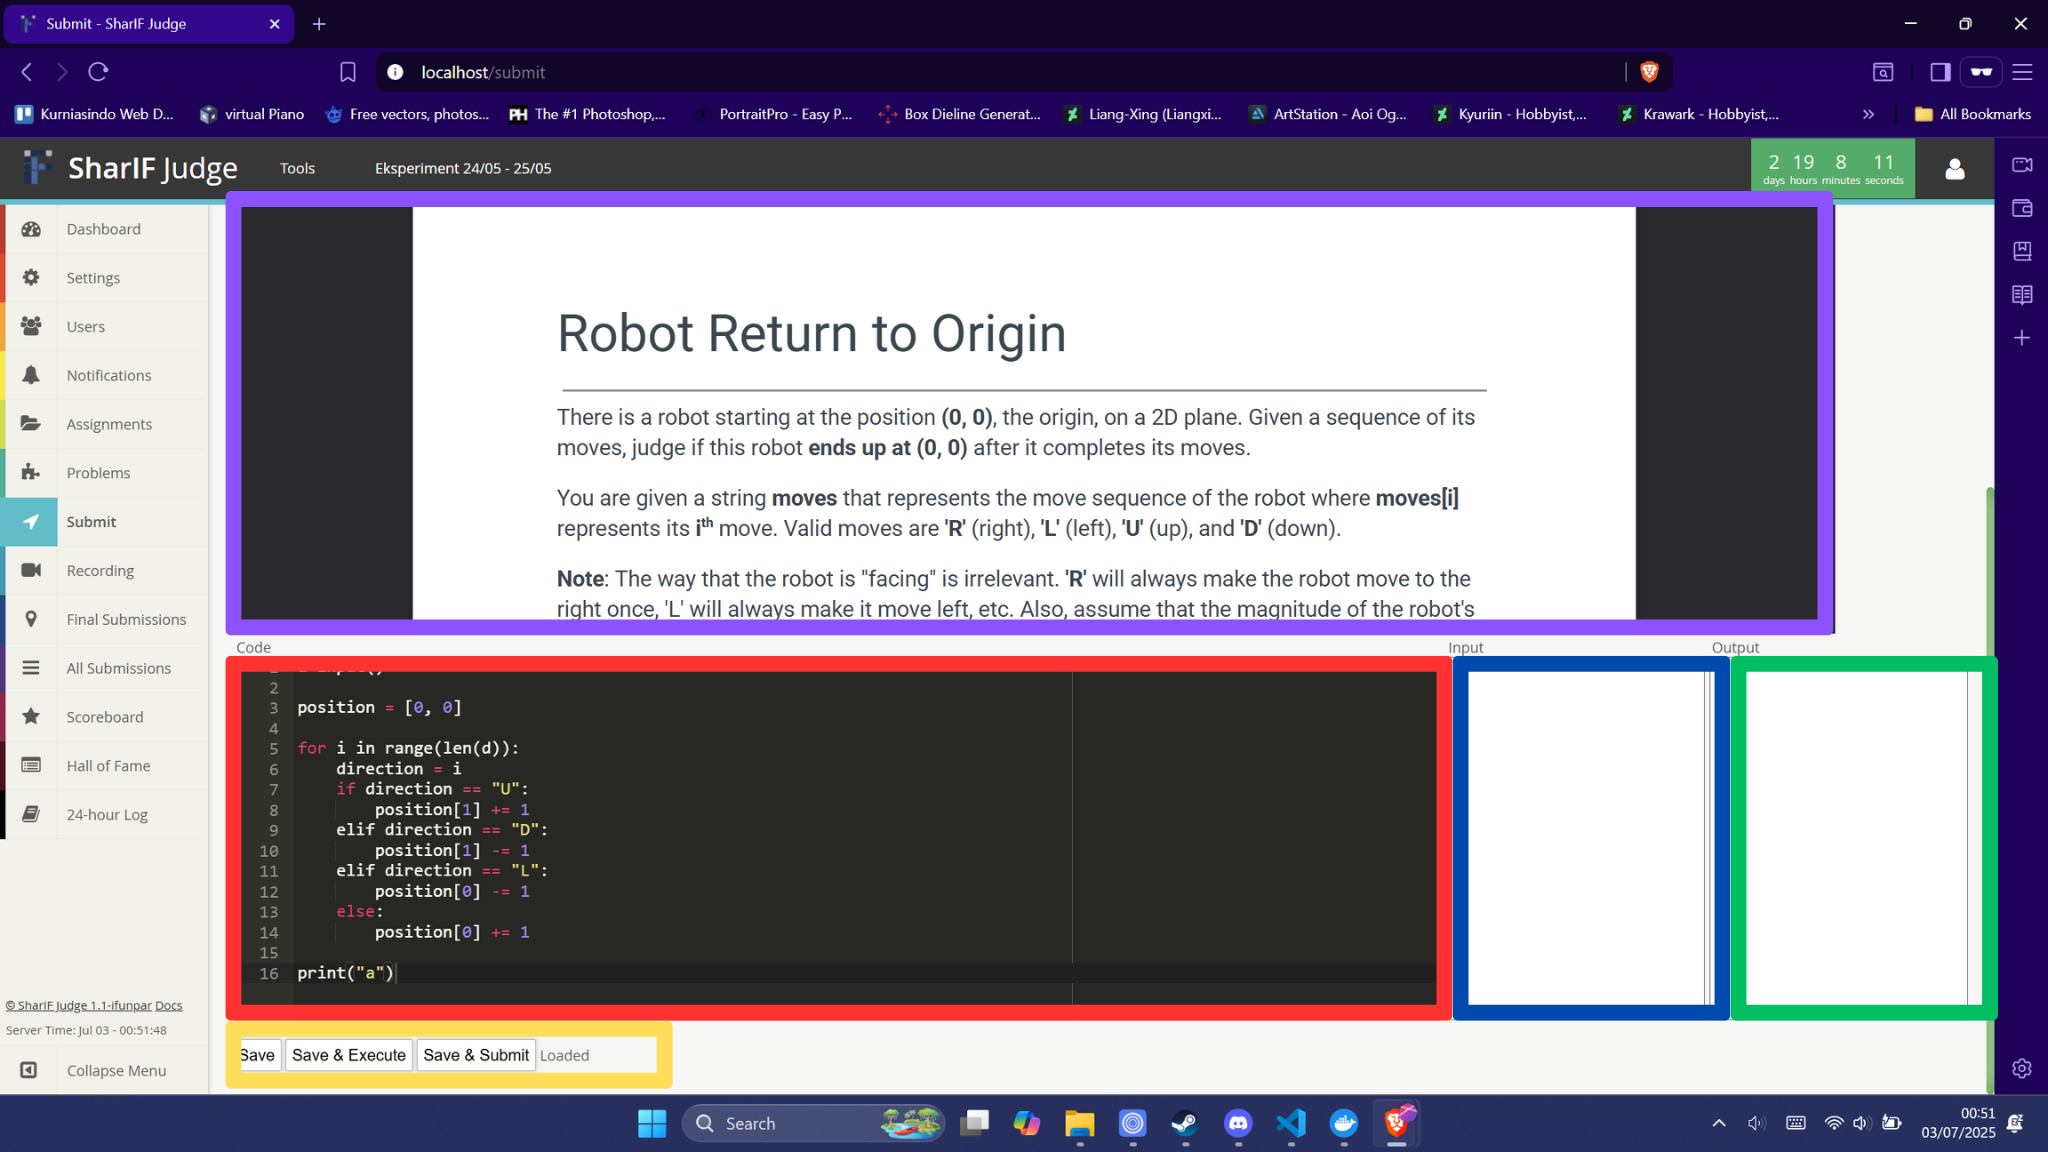
\includegraphics[width=\textwidth]{editor-kode-colored.png}
	\caption{Editor Kode SharIF Judge}
	\label{fig:3:1:editorkode}
\end{figure}

Fitur Execute dan Submit merupakan inti dari alur kerja SharIF Judge. Execute memungkinkan pengguna menguji kode secara mandiri, sementara Submit mengirim kode ke sistem penilaian otomatis untuk evaluasi akhir. Desain warna yang konsisten ini memudahkan pengguna dalam mengidentifikasi fungsi masing-masing komponen selama sesi pemrograman.

\section{Analisis Pola Kecurangan pada Rekaman Ketikan}

Berdasarkan indikator yang dijelaskan pada Bagian~\ref{sec:2:deteksikecurangan}, sistem pemutaran ulang SharIF Judge akan mendeteksi pola perilaku yang mencurigakan. Bagian ini menjelaskan implementasi dari indikator-indikator tersebut serta metode analisis yang digunakan untuk mengidentifikasi kecurangan.

\subsection{Analisis Perubahan Kode}

Sistem menghitung code churn rate dengan membandingkan jumlah karakter yang ditambahkan, dihapus selama sesi pengerjaan. Rekaman ketikan yang menunjukkan perubahan minimal seperti angka code churn rate mendekati angka satu, akan ditandai sebagai potensi kecurangan. Tetapi code churn rate ini akan dibandingkan dengan keseluruhan code churn rate pada permasalahan tersebut agar lebih memiliki toleransi jika permasalahan yang diberikan merupakan permasalahan yang mudah.

\subsection{Analisis Aktivitas Navigasi}

Sistem akan merekam setiap peristiwa kehilangan fokus pada IDE, termasuk perpindahan tab browser. Pola kecurangan ditandai dengan frekuensi navigasi tinggi dalam waktu per jam yang berkorelasi.

\subsection{Analisis Pengukuran Jeda Berpikir}

Durasi jeda antara ketikan dianalisis untuk mengidentifikasi ketidakwajaran. Pada pemrograman alami, jeda lebih dari 10 detik sering muncul saat mahasiswa merancang solusi atau menguji logika. Rekaman yang menunjukkan ketikan berkelanjutan tanpa jeda atau jeda sangat singkat seperti 5 detik dan sering dianggap sebagai indikasi copy-paste. Sebaliknya juga jika jeda panjang juga dapat menjadi potensi kecurangan. Tetapi pengukuran ini juga akan dibandingkan dengan rata-rata pada permasalahan agar lebih toleransi.

\subsection{Analisis Deteksi Debugging}

Aktivitas debugging dapat diindikasikan dari frekuensi eksekusi kode, perubahan input, modifikasi pada area spesifik, dan perubahan hasil output dengan input yang sama. Semua aktivasitas tersebut akan direkam dan jika tidak ada indikasi debugging tersebut, kecurangan diduga terjadi.

\subsection{Analisis \textit{Copy-Pasting}}

Jika pada rekaman terdapat pemasukkan kode yang besar tanpa melakukan penghapusan dengan besar yang sama, maka dapat diduga bahwa dia mendapatkan kode eksternal.

\section{Analisis Sistem Usulan}
\label{sec:3:sistemusulan}

Pembuatan sistem pemutaran ulang ketikan membutuhkan 4 fitur baru yaitu fitur perekaman perubahan, fitur penyimpanan rekaman perubahan, fitur melihat daftar rekaman yang ada, dan fitur untuk memutar ulang rekaman. Gambar \ref{fig:3:usecase} menunjukkan bagaimana fitur baru akan berinteraksi dengan sistem SharIF Judge dan pengguna. Berikut merupakan penjelasan mengenai fitur-fitur yang akan ditambahkan pada SharIF Judge untuk membangun sistem perekaman ketikan ditandai dengan warna biru dalam bagan \textit{usecase} tersebut.

\begin{figure}[H]
	\centering
	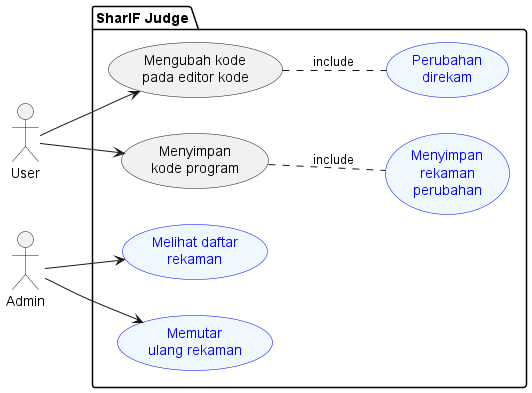
\includegraphics[width=0.75\textwidth]{analisis/usecase.png}
	\caption{Usecase analisis sistem usulan}
	\label{fig:3:usecase}
\end{figure}

\subsection{Fitur perekaman perubahan atau event}
\label{sub:3:2:rekam}
Fitur perekaman pada editor kode bukan hanya perubahan text melainkan pada seluruh kejadian atau \textit{event} yang terjadi pada editor kode seperti contohnya adalah perubahan posisi kursor maupun pilihan pada kode. Fitur perekaman perubahan akan otomatis oleh browser dengan bantuan \textit{JavaScript} yang ada pada browser pengguna dan akan dijalankan saat sebuah \textit{event} terjadi pada editor kode. Fitur ini membutuhkan perubahan pada \textit{Assets} \verb|shj_submit.js| untuk merekam event yang dibutuhkan.

\subsubsection{Sequence Diagram}
Gambar \ref{fig:3:2:seqdia_rekam} merupakan sebuah \textit{sequence} diagram yang menunjukkan bagaimana fitur perekaman perubahan atau event akan berintegrasi dengan sistem IDE akan bekerja pada SharIF Judge.
\begin{figure}[H]
	\centering
	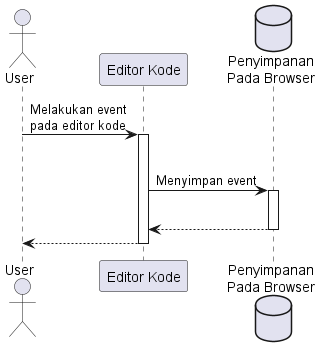
\includegraphics[scale=0.7]{analisis/seqdia_rekam.png}
	\caption{Sequence Diagram Fitur Perekaman Perubahan}
	\label{fig:3:2:seqdia_rekam}
\end{figure}

\subsection{Fitur penyimpanan rekaman perubahan}
\label{sub:3:2:save}
Fitur penyimpanan rekaman perubahan akan dilakukan secara otomatis saat pengguna melakukan tindakan menyimpan kode program. Fitur penyimpanan rekaman akan berintegrasi dengan fitur penyimpanan kode program yang sudah ada. Pada fitur ini daftar rekaman akan diperbaharui dengan adanya rekaman baru atau perubahan pada \textit{file} rekaman. Fitur ini membutuhkan perubahan pada \textit{Assets} \verb|shj_submit.js|, \textit{Controller} \verb|Submit|, \textit{Model} baru untuk \verb|Rekaman| untuk mengirimkan data rekaman, mendapatkan data rekaman dan mencatat data rekaman.

\subsubsection{Sequence Diagram}
Gambar \ref{fig:3:2:seqdia_save} merupakan sebuah \textit{sequence} diagram yang menunjukkan bagaimana fitur penyimpanan rekaman perubahan akan berintegrasi dengan sistem IDE akan bekerja pada SharIF Judge.
\begin{figure}
	\centering
	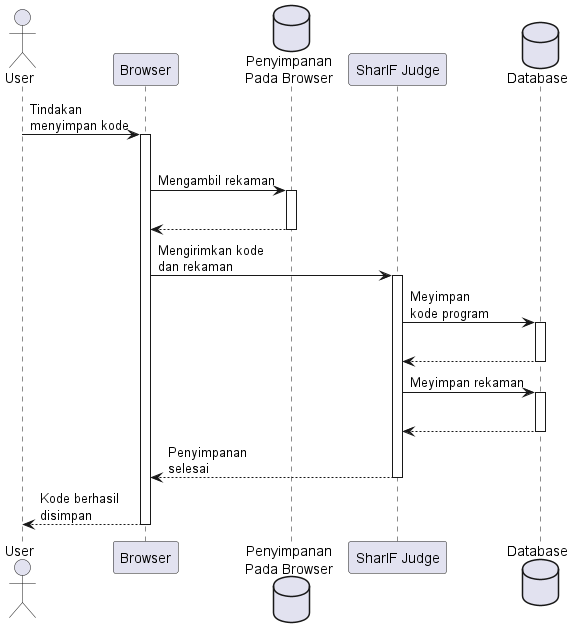
\includegraphics[scale=0.5]{analisis/seqdia_save.png}
	\caption{Sequence Diagram Fitur Penyimpanan Rekaman}
	\label{fig:3:2:seqdia_save}
\end{figure}

\subsection{Fitur melihat daftar rekaman}
\label{sub:3:2:lookup}
Pada sistem pemutaran ulang ketikan dibutuhkannya sebuah halaman baru yang akan dinamakan halaman rekaman. Pada halaman ini akan ditampilkan daftar rekaman untuk \textit{assignment} yang dipilih pada halaman \textit{Assignment}. Fitur ini akan dijalankan pada saat halaman rekaman dimuat ke dalam browser oleh SharIF Judge, dimana data yang dimasukkan ke dalam halaman rekaman adalah daftar rekaman tersebut dan beberapa data yang dibutuhkan. Fitur ini membutuhkan \textit{View} dan \textit{Controller} baru untuk membuat sebuah halaman baru untuk menunjukkan list rekaman yang ada. Fitur ini juga membuatkan penambahan pada \textit{Model} Recording untuk mendapatkan daftar rekaman yang akan ditampilkan.

\subsubsection{Sequence Diagram}
Gambar \ref{fig:3:2:seqdia_lookup} merupakan \textit{sequence} diagram yang menunjukkan bagaimana sistem akan bekerja saat user akan membuka halaman rekaman pada SharIF Judge.
\begin{figure}
	\centering
	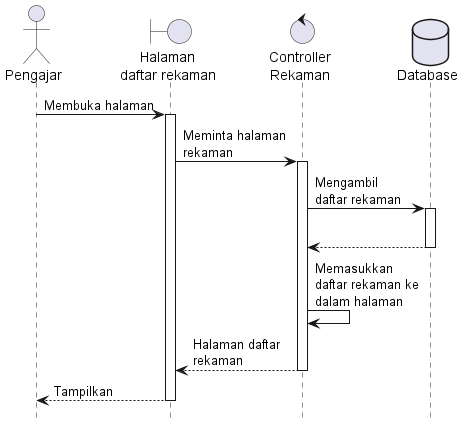
\includegraphics[scale=0.525]{analisis/seqdia_lookup.png}
	\caption{Sequence Diagram Membuka Halaman Rekaman}
	\label{fig:3:2:seqdia_lookup}
\end{figure}

\subsection{Fitur pemutaran ulang rekaman}
\label{sub:3:2:seerecording}

Fitur pemutaran ulang rekaman akan membuat satu buah rekaman dalam daftar rekaman dalam halaman rekaman dapat ditekan oleh pengguna untuk menandakan bahwa sebuah rekaman dipilih untuk dijalankan. Saat sebuah rekaman dipilih, browser akan meminta data rekaman kepada SharIF Judge dan dengan bantuan \textit{JavaScript} akan melakukan pemutaran ulang rekaman pada sebuah editor kode yang tidak dapat diubah dalam halaman rekaman. Fitur ini membatkan penambahan ada \textit{Controller} Rekaman dan penambahan halaman baru atau \textit{View} baru untuk menunjukkan sebuah rekaman. Fitur ini juga membutuhkan \textit{Assets} baru untuk memutar ulang dari data rekaman yang didapat.

\subsubsection{Sequence Diagram}
Gambar \ref{fig:3:2:seqdia_seerecording} merupakan \textit{sequence} diagram yang menunjukkan bagaimana sistem SharIF Judge bekerja dari pemilihan rekaman hingga pemutaran ulang rekaman akan terjadi.
\begin{figure}[H]
	\centering
	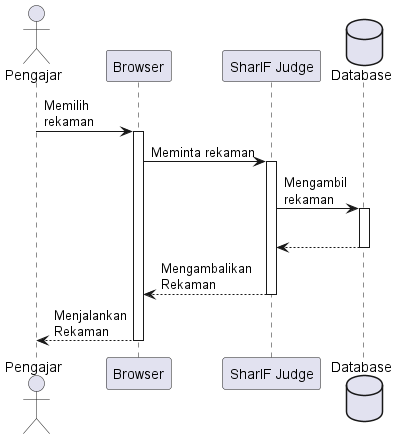
\includegraphics[scale=0.525]{analisis/seqdia_seerecording.png}
	\caption{Sequence Diagram Membuka Halaman Rekaman}
	\label{fig:3:2:seqdia_seerecording}
\end{figure}